%%%%%%%%%%%%%%%%%%%%%%%%%%%%%%%%%%%%%%%%%%%%%%%%%%%%%%%%%%%%%%%%%%%%%%
% Lớp 11 | Hàm số mũ và hàm số lôgarít | Phương trình, bất phương trình mũ và lôgarít
% Dạng 1D6?4-2: Phương trình mũ, lôgarít cơ bản
% Số câu: 188  (sinh tự động bởi tach_cau.py; từ nay thầy sửa trực tiếp file này)
%%%%%%%%%%%%%%%%%%%%%%%%%%%%%%%%%%%%%%%%%%%%%%%%%%%%%%%%%%%%%%%%%%%%%%

%%%%%%%%%%%%%%%% TRẮC NGHIỆM 4 PHƯƠNG ÁN %%%%%%%%%%%%%%%%

% nguồn: Ok_Toan11_TracNghiem_Lan2
\begin{ex}%[1D6N4-2]%[ma:1eb840ed]
	Nghiệm của phương trình  $5^x=10$ là
	\choice 
		{\True $x=\log_5 10$} 
		 {$x=\log_{10} 5$}
		{$x=2$} 
		 {$x=\dfrac{1}{2}$}
	 \loigiai{
		$5^x=10 \Leftrightarrow x=\log_5  10$.
	 }
\end{ex}

% nguồn: Ok_Toan11_TracNghiem_Lan2
\begin{ex}%[1D6N4-2]%[ma:ca8ae412]
	Nghiệm  của phương trình ${{\log }_3}\left( 2x+1 \right)=2$ là
	\choice 
		{  $x=2$}
		{\True  $x=4$}
		{ $x=-\dfrac{1}{2}$} 
		{ $x=-2$} 
	 \loigiai{
		 Điều kiện $x>-\dfrac{1}{2}$.\\
		Ta có ${{\log }_3}\left( 2x+1 \right)=2\Leftrightarrow 2x+1=9\Leftrightarrow x=4$.\\ 
	Vậy phương trình có  nghiệm là $x=4$.}
\end{ex}

% nguồn: Ok_Toan11_TracNghiem_Lan2
\begin{ex}%[1D6N4-2]%[ma:74ad84bf]
	Phương trình ${{\log}_{\sqrt{3}}}\left(x-2\right)+{{\log}_3}{{\left(x-4\right)}^2}=0$ có hai nghiệm $x_1,x_2$. Khi đó  $S={{\left({x_1}-x_2\right)}^2}$ bằng
	 \choice
		{1} 
		{9} 
		 {7}
		{\True 2} 
	\loigiai{Điều kiện $2<x\ne 4$.\\ 
		Với điều kiện trên, phương  trình đã cho trở thành\\
		$2{{\log}_3}\left(x-2\right)+2{{\log}_3}\left|x-4\right|=0\Leftrightarrow  {{\log}_3}\left(x-2\right)\left|x-4\right|=0\Leftrightarrow \left(x-2\right)\left|x-4\right|=1$\\
		$\Leftrightarrow  \hoac{& \heva{x\ge 4\\
		& \left(x-2\right)\left(x-4\right)=1\\ 
		} \\ 
		 & \heva{x<4\\
		& \left(x-2\right)\left(x-4\right)=-1\\ 
		}  \\
		}\Leftrightarrow \hoac{& \heva{x\ge 4\\ 
		&  {x^2}-6x+7=0\\
		}  \\
		& \heva{x<4\\ 
		 & {x^2}-6x+9=0\\
		} \\ 
		}\Leftrightarrow \hoac{&  x=3+\sqrt{2} \\
		 & x=3.
		 }$\\
		Kết hợp điều kiện,  phương trình có nghiệm $x_1=3+\sqrt{2};x_2=3$. Vậy $S=2$.
	} 
\end{ex}

% nguồn: Ok_Toan11_TracNghiem_Lan2
\begin{ex}%[1D6N4-2]%[ma:c96fcf79]
	 Tập nghiệm của phương trình ${{\log}_2}\left(-x^2+4x-3\right)-1={{\log}_2}\left(\dfrac{5}{2}-x \right)$ là
	\choice 
		 {$\left\{2;4\right\}$}
		 {$\{4\}$}
		 {$\left\{2;3\right\}$}
		{\True  $\{2\}$}
	\loigiai{Điều kiện  xác định $\heva{&-x^2+4x-3>0\\
		 & \dfrac{5}{2}-x>0\\
		 }\Leftrightarrow \heva{& 1<x<3\\
		& x<\dfrac{5}{2}  \\
		}\Leftrightarrow 1<x<\dfrac{5}{2}$.\\ 
		Ta  có: ${{\log}_2}\left(-x^2+4x-3\right)-1={{\log}_2}\left(\dfrac{5}{2}-x \right)\Leftrightarrow {{\log}_2}\left(-x^2+4x-3\right)={{\log}_2}\left(\dfrac{5}{2}-x \right)+{{\log}_2}2$\\
		$\Leftrightarrow-x^2+4x-3=5-2x\Leftrightarrow  {x^2}-6x+8=0\Leftrightarrow \hoac{& x=2\left(tm \right) \\
		&  x=4\left(l \right). \\
		 }$\\
	Nghiệm của phương trình  là $x=2$.}
\end{ex}

% nguồn: Ok_Toan11_TracNghiem_Lan2
\begin{ex}%[1D6N4-2]%[ma:f036a260]
	Nghiệm của phương trình $\log_2(x-5)=3$  là
	\choice 
		{$x=21$} 
		{$x=11$} 
		{\True $x=13$} 
		{$x=14$} 
	\loigiai{ 
		 Điều kiện xác định $x>5$.\\
		Phương trình $\log_2(x-5)=3 \Leftrightarrow x-5=8 \Leftrightarrow  x=13$.\\
		Vậy phương trình có nghiệm  $x=13$.
	 }
\end{ex}

% nguồn: Ok_Toan11_TracNghiem_Lan2
\begin{ex}%[1D6N4-2]%[ma:cebc3ba6]
	Nghiệm của  phương trình ${{\log }_2}\left( x-1 \right)=3$ là
	 \choice
		{\True  $x=9$}
		{  $x=5$}
		 { $x=1$}
		 { $x=10$}
	 \loigiai{
		Điều kiện  $x>1$.\\
	Ta có: ${{\log }_2}\left( x-1  \right)=3\Leftrightarrow x-1=2^3\Leftrightarrow x=9\left( \text{tm} \right)$.}
\end{ex}

% nguồn: Ok_Toan11_TracNghiem_Lan2
\begin{ex}%[1D6N4-2]%[ma:39a92cd3]
	Nghiệm của phương trình  $\log_3(x-2)=2$ là
	 \choice
		 {\True $x=11$}
		{$x=10$} 
		 {$x=7$}
		 {$x=8$}
	 \loigiai{
		Điều kiện xác định: $x-2>0 \Leftrightarrow x>2$.\\ 
		Phương trình tương đương $\log_3(x-2)=2 \Leftrightarrow  x-2=3^2 \Leftrightarrow x-2=9 \Leftrightarrow x=11$.\\
		Giá trị $x=11$ thỏa mãn  điều kiện.
	} 
\end{ex}

% nguồn: Ok_Toan11_TracNghiem_Lan2
\begin{ex}%[1D6N4-2]%[ma:0e1885f4]
	Tìm nghiệm  của phương trình $\log_{25}(x+1)=\dfrac{1}{2}$.
	\choice 
		{$x=6$} 
		 {\True $x=4$}
		{$x=\dfrac{23}{2}$} 
		 {$x=-6$}
	 \loigiai{
		Điều kiện: $x+1>0 \Leftrightarrow x>-1$.\\ 
		Phương trình đã cho  tương đương với $\log_{25}(x+1)=\dfrac{1}{2} \Leftrightarrow x+1=25^{\tfrac{1}{2}} \Leftrightarrow x+1=\sqrt{25} \Leftrightarrow x+1=5 \Leftrightarrow x=4$ (thỏa mãn).
	 }
\end{ex}

% nguồn: Ok_Toan11_TracNghiem_Lan2
\begin{ex}%[1D6N4-2]%[ma:3cd7e573]
	Số nghiệm thực của phương trình  $3{{\log}_3}\left(x-1\right)-{{\log}_{\tfrac{1}{3}}}{{\left(x-5\right)}^3}=3$ là
	 \choice
		 {$3$}
		{\True $1$} 
		 {$2$}
		 {$0$}
	\loigiai{Điều  kiện $x>5$.\\
		Phương trình tương đương:  $3{{\log}_3}\left(x-1\right)-{{\log}_{\tfrac{1}{3}}}{{\left(x-5\right)}^3}=3\Leftrightarrow 3{{\log}_3}\left(x-1\right)+3{{\log}_3}\left(x-5\right)=3$\\ $\Leftrightarrow {{\log}_3}\left(x-1\right)+{{\log}_3}\left(x-5\right)=1\Leftrightarrow {{\log}_3}\left[\left(x-1\right)\left(x-5\right) \right]=1$ $\Leftrightarrow \left(x-1\right)\left(x-5\right)=3$\\
		$\Leftrightarrow {x^2}-6x+2=0\Leftrightarrow x=3\pm \sqrt{7}$.\\ 
	Đối chiếu điều  kiện suy ra phương trình có $1$ nghiệm $x=3+\sqrt{7}$.}
\end{ex}

% nguồn: Ok_Toan11_TracNghiem_Lan2
\begin{ex}%[1D6N4-2]%[ma:27a57889]
	Có tất cả bao nhiêu giá trị của tham  số $m$ để phương trình $${{\log}_3}(x+2)={{\log}_3}\left[{x^2}-(m-1)x+m^2-6m+2\right]$$ có hai nghiệm trái dấu?
	 \choice
		{\True  $4$}
		{$3$} 
		 {vô số}
		{$5$} 
	\loigiai{Phương trình  đã cho tương đương:\\
		$\heva{& x>-2\\ 
		& {x^2}-(m-1)x+m^2-6m+2=x+2\\ 
		 }
		\Leftrightarrow  \heva{& x>-2\\
		& {x^2}-mx+m^2-6m=0  \left(* \right) \\
		}$\\ 
		Yêu cầu đề bài khi và  chỉ khi phương trình $\left(* \right)$ có hai nghiệm $x_1,x_2$ thỏa $-2<x_1<0<x_2$.\\
		$\Leftrightarrow \heva{& {x_1}.x_2<0\\ 
		& \left({x_1}+2\right)\left({x_2}+2\right)>0\\ 
		}\Leftrightarrow \heva{& {x_1}.x_2<0\\ 
		& {x_1}{x_2}+2\left({x_1}+x_2\right)+4>0\\ 
		}\Leftrightarrow \heva{& {m^2}-6m<0\\ 
		& {m^2}-4m+4>0\\ 
		}\Leftrightarrow \heva{& 0<m<6\\ 
		&  m\ne 2.\\
		 }$
		Vì $m\in \mathbb{Z}$  nên $m\in \left\{1;3;4;5\right\}$.\\
	Suy ra có $4$ giá trị của tham số $m$ thoả mãn  điều kiện bài toán.}
\end{ex}

% nguồn: Ok_Toan11_TracNghiem_Lan2
\begin{ex}%[1D6N4-2]%[ma:11834d49]
	 Phương trình ${{\log}_5}\left(2x+3\right)={{\log}_5}\left(x+2\right)$ có nghiệm là
	 \choice
		 {$x=1$}
		{$x=5$} 
		{\True  $x=-1$}
		{$x=-5$} 
	\loigiai{Điều  kiện $\heva{& 2x+3>0\\
		&  x+2>0\\
		}\Leftrightarrow  \heva{& x>-\dfrac{3}{2} \\
		 & x>-2\\
		}\Leftrightarrow x>-\dfrac{3}{2}$.\\ 
		Phương trình ${{\log}_5}\left(2x+3\right)={{\log}_5}\left(x+2\right)\Leftrightarrow 2x+3=x+2\Leftrightarrow x=-1$.\\ 
	Vậy nghiệm  của phương trình là $x=-1$.}
\end{ex}

% nguồn: Ok_Toan11_TracNghiem_Lan2
\begin{ex}%[1D6N4-2]%[ma:987bdf81]
	Nghiệm của phương  trình $\log_2(x-1)=3$ là
	 \choice
		 {$x=10$}
		{$x=8$} 
		{\True $x=9$} 
		 {$x=7$}
	 \loigiai{
		 Điều kiện xác định: $x-1>0 \Leftrightarrow x>1$.\\
		 Phương trình tương đương $x-1=2^3 \Leftrightarrow x-1=8 \Leftrightarrow x=9$.\\
		Giá trị  $x=9$ thỏa mãn điều kiện.
	} 
\end{ex}

% nguồn: Ok_Toan11_TracNghiem_Lan2
\begin{ex}%[1D6N4-2]%[ma:db9ef2fb]
	Nghiệm của phương  trình $\ln(3x)=2$ là
	 \choice
		{$x=\mathrm{e}^3$} 
		 {$x=\dfrac{\mathrm{e}^3}{2}$}
		 {$x=\mathrm{e}^2$}
		 {\True $x=\dfrac{\mathrm{e}^2}{3}$}
	 \loigiai{
		$$\ln(3x)=2  \Leftrightarrow 3x=\mathrm{e}^2 \Leftrightarrow x=\dfrac{\mathrm{e}^2}{3}.$$
	} 
\end{ex}

% nguồn: Ok_Toan11_TracNghiem_Lan2
\begin{ex}%[1D6N4-2]%[ma:4e72a39c]
	Nghiệm của  phương trình $\log_2(x+6)=5$ là:
	 \choice
		 {$x=4$}
		{$x=19$} 
		 {$x=38$}
		 {\True $x=26$}
	\loigiai{ 
		Điều  kiện xác định: $x+6>0 \Leftrightarrow x>-6$.\\
		Phương trình tương đương $\log_2(x+6)=5 \Leftrightarrow x+6=2^5 \Leftrightarrow x+6=32 \Leftrightarrow  x=26$.\\
		Giá trị $x=26$  thỏa mãn điều kiện.
	} 
\end{ex}

% nguồn: Ok_Toan11_TracNghiem_Lan2
\begin{ex}%[1D6N4-2]%[ma:9a3b2cf7]
	Phương  trình ${{\log}_5}(x^2+2x+1)=2$ có tập nghiệm là.
	 \choice
		 {$\{4\}$}
		{\True $\left\{-6;4\right\}$} 
		 {$\left\{4;6\right\}$}
		 {$\left\{-2;4\right\}$}
	\loigiai{Điều kiện $x^2+2x+1>0\Leftrightarrow {{(x+1)}^2}>0\Leftrightarrow \forall  x\ne-1$.\\
		 Ta có:\\
		$\begin{aligned}
		& {{\log}_5}(x^2+2x+1)=2\Leftrightarrow {x^2}+2x+1=25\Leftrightarrow {x^2}+2x-24=0\Leftrightarrow \hoac{&  {x_1}=-6\\
		& {x_2}=4.\\ 
		 }(tm) \\
		 & \\
	\end{aligned}$.\\
 Vậy tập nghiệm của phương trình $S=\left\{-6;4\right\}$.}
\end{ex}

% nguồn: Ok_Toan11_TracNghiem_Lan2
\begin{ex}%[1D6N4-2]%[ma:4a454726]
	Số nghiệm của phương trình  ${{\log}_{\tfrac{1}{3}}}\left({x^2}-3x-1\right)+{{\log}_3}\left(2-x \right)=0$
	\choice 
		{\True $1$} 
		{$3$} 
		 {$2$}
		 {$0$}
	 \loigiai{Điều kiện xác định $\heva{& {x^2}-3x-1>0\\
		& 2-x>0. 
		 }$\\
		Phương trình tương đương:\\ 
		$\begin{aligned}
		& {{\log}_{\tfrac{1}{3}}}\left({x^2}-3x-1\right)+{{\log}_3}\left(2-x  \right)=0\Leftrightarrow-{{\log}_3}\left({x^2}-3x-1\right)+{{\log}_3}\left(2-x \right)=0\\
		& \Leftrightarrow {{\log}_3}\left({x^2}-3x-1\right)={{\log}_3}\left(2-x  \right)\Leftrightarrow {x^2}-2x-3=0\Leftrightarrow \hoac{& x=-1\\
		 & x=3.
		 } \\
	\end{aligned}$\\
Đối  chiếu với đk thì $x=-1$ là nghiệm của phương trình.}
\end{ex}

% nguồn: Ok_Toan11_TracNghiem_Lan2
\begin{ex}%[1D6N4-2]%[ma:cf37fe80]
	Số nghiệm của phương trình ${{\log}_2}{x^2}=2{{\log}_2}(3x+4)$  là
	 \choice
		 {$2$}
		 {$0$}
		 {\True $1$}
		 {$3$}
	\loigiai{Điều kiện $\heva{&  {x^2}>0\\
		 & 3x+4>0\\
		}\Leftrightarrow \heva{& x\ne  0\\
		&  x>-\dfrac{4}{3}.\\
		 }$\\
		Phương trình tương đương:\\ ${{\log}_2}{x^2}=2{{\log}_2}(3x+4)\Rightarrow  {x^2}={{\left(3x+4\right)}^2}\Leftrightarrow 8x^2+24x+16=0\Leftrightarrow \hoac{& x=-1\\
		&  x=-2.\\
		}$.\\ 
	So điều kiện  $\Rightarrow x=-1$}
\end{ex}

% nguồn: Ok_Toan11_TracNghiem_Lan2
\begin{ex}%[1D6N4-2]%[ma:4a3157ca]
	Nghiệm của phương trình  ${{\log }_2}x+{{\log }_2}3=0$ là
	\choice 
		{ $x=-3$} 
		{ $x=\dfrac{1}{8}$} 
		{\True $x=\dfrac{1}{3}$} 
		{ $x=3$} 
	\loigiai{ 
		Ta có:  ${{\log }_2}x+{{\log }_2}3=0\Leftrightarrow {{\log }_2}x=-{{\log }_2}3
	\Leftrightarrow {{\log }_2}x={{\log }_2}\dfrac{1}{3}\Leftrightarrow x=\dfrac{1}{3}$.} 
\end{ex}

% nguồn: Ok_Toan11_TracNghiem_Lan2
\begin{ex}%[1D6N4-2]%[ma:b11f58df]
	Nghiệm của phương trình  $5^{2x-4}=25$ là:
	\choice 
		{\True $x=3$} 
		 {$x=2$}
		 {$x=1$}
		{$x=-1$} 
	 \loigiai{
		Ta có $5^{2x-4}=25 \Leftrightarrow 5^{2x-4}=5^2 \Leftrightarrow 2x-4=2 \Leftrightarrow 2x=6  \Leftrightarrow x=3$.
	 }
\end{ex}

% nguồn: Ok_Toan11_TracNghiem_Lan2
\begin{ex}%[1D6N4-2]%[ma:90f804f9]
	Số nghiệm của phương trình ${{\log}_3}\left({x^2}+2\right)=3$ là 
	\choice 
		{$0$} 
		{\True  $2$}
		 {$1$}
		{$3$} 
	\loigiai{Điều kiện xác định của phương trình:  $x\in \mathbb{R}$.\\
		Ta  có: ${{\log}_3}\left({x^2}+2\right)=3\Leftrightarrow {x^2}+2=3^3\Leftrightarrow {x^2}=25\Leftrightarrow \hoac{& x=5\\
		&  x=-5.\\
		 }(tm)$\\
	Vậy,  phương trình trên có hai nghiệm.}
\end{ex}

% nguồn: Ok_Toan11_TracNghiem_Lan2
\begin{ex}%[1D6N4-2]%[ma:5d2cd9c4]
	Nghiệm của  phương trình $\log_2(3x-4)=-1$ là:
	\choice 
		 {$x=2$}
		 {\True $x=\dfrac{3}{2}$}
		 {$x=\dfrac{7}{6}$}
		{$x=\dfrac{5}{3}$} 
	 \loigiai{
		$$\log_2(3x-4)=-1 \Leftrightarrow 3x-4=2^{-1}=\dfrac{1}{2}  \Leftrightarrow x=\dfrac{3}{2}.$$
	} 
\end{ex}

% nguồn: Ok_Toan11_TracNghiem_Lan2
\begin{ex}%[1D6N4-2]%[ma:cf328851]
	Nghiệm của phương trình $7^x=2$  là
	 \choice
		{\True $x=\log_7  2$}
		{$x=\log_2  7$}
		{$x=\dfrac{2}{7}$} 
		 {$x=\sqrt{7}$}
	\loigiai{ 
		Ta có $7^x=2 \Leftrightarrow x=\log_7  2$.
	} 
\end{ex}

% nguồn: Ok_Toan11_TracNghiem_Lan2
\begin{ex}%[1D6N4-2]%[ma:1d109d79]
	Tập nghiệm $S$ của phương trình ${{\log}_2}\left(x-1\right)={{\log}_2}\left(2x+1\right)$ là 
	 \choice
		 {$S=\{0\}$}
		{$S=\{2\}$} 
		{$S=\{-2\}$} 
		{\True  $S=\varnothing$}
	\loigiai{Ta  có: ${{\log}_2}\left(x-1\right)={{\log}_2}\left(2x+1\right)\Leftrightarrow \heva{& x-1>0\\
		& x-1=2x+1\\ 
		}$ $\Leftrightarrow \heva{&  x>1\\
		&  x=-2.
		}(l)$\\ 
	Vậy phương trình  vô nghiệm hay $S=\varnothing$.}
\end{ex}

% nguồn: Ok_Toan11_TracNghiem_Lan2
\begin{ex}%[1D6N4-2]%[ma:5f76e034]
	 Nghiệm của phương trình $7^x=3$ là
	 \choice
		{$x=\dfrac{3}{7}$} 
		 {$x=\sqrt[3]{7}$}
		{\True  $x=\log_7 3$}
		{$x=\log_3  7$}
	\loigiai{ 
		Ta có  $7^x=3 \Leftrightarrow x=\log_7 3$.
	} 
\end{ex}

% nguồn: Ok_Toan11_TracNghiem_Lan2
\begin{ex}%[1D6N4-2]%[ma:a00663dc]
	 Nghiệm của phương trình ${{\log}_2}(2x-3)={{\log}_2}(x+1)$ là
	\choice 
		{$x=2$} 
		{$x=-2$} 
		{\True $x=4$} 
		{$x=-4$} 
	\loigiai{Điều kiện $x>\dfrac{3}{2}$.\\ 
		Phương trình tương đương: $2x-3=x+1\Leftrightarrow x=4(tm)$.\\ 
	Vậy phương trình có  nghiệm $x=4$.}
\end{ex}

% nguồn: Ok_Toan11_TracNghiem_Lan2
\begin{ex}%[1D6N4-2]%[ma:2a9fb37f]
	Nghiệm của  phương trình $\log_2(3x)=3$ là:
	\choice 
		 {$x=3$}
		 {$x=2$}
		{\True $x=\dfrac{8}{3}$} 
		{$x=\dfrac{1}{2}$} 
	\loigiai{ 
		Điều kiện xác  định: $3x>0 \Leftrightarrow x>0$.\\
		Phương trình đã cho tương đương $\log_2(3x)=3 \Leftrightarrow 3x=2^3 \Leftrightarrow 3x=8  \Leftrightarrow x=\dfrac{8}{3}$.\\
		Giá trị $x=\dfrac{8}{3}$ thỏa mãn điều  kiện.
	} 
\end{ex}

% nguồn: Ok_Toan11_TracNghiem_Lan2
\begin{ex}%[1D6N4-2]%[ma:ccc9ec1e]
	Giải phương trình  $\log_3 (x-1)=2$.
	\choice 
		{$x=7$} 
		 {$x=9$}
		 {$x=8$}
		 {\True $x=10$}
	\loigiai{ 
		Điều kiện $x>1$. 
		 $$\log_3(x-1)=2 \Leftrightarrow x-1=3^2 \Leftrightarrow x=10.$$
	 }
\end{ex}

% nguồn: Ok_Toan11_TracNghiem_Lan2
\begin{ex}%[1D6N4-2]%[ma:f119a4a3]
	Nghiệm của  phương trình $\log_3(x-1)=2$ là
	\choice 
		 {$x=8$}
		 {$x=9$}
		 {$x=7$}
		 {\True $x=10$}
	\loigiai{ 
		Điều kiện xác định: $x-1>0 \Leftrightarrow x>1$.\\ 
		Phương trình  tương đương $x-1=3^2 \Leftrightarrow x-1=9 \Leftrightarrow x=10$.\\
		Giá trị $x=10$ thỏa  mãn điều kiện.
	} 
\end{ex}

% nguồn: Ok_Toan11_TracNghiem_Lan2
\begin{ex}%[1D6N4-2]%[ma:12f20ee7]
	Gọi $S$ là tập nghiệm của phương  trình ${{\log}_2}\left(x-3\right)+{{\log}_2}\left(x-1\right)=3$. Tổng tất cả các phần tử của $S$bằng
	 \choice
		{$4$} 
		 {\True $5$}
		{$6$} 
		 {$2$}
	\loigiai{Điều  kiện xác định $x>3$.\\
		 Khi đó: ${{\log}_2}\left(x-3\right)+{{\log}_2}\left(x-1\right)=3\Leftrightarrow {{\log}_2}\left[\left(x-1\right)\left(x-3\right) \right]=3$\\
		$\Leftrightarrow {x^2}-4x+3=8\Leftrightarrow {x^2}-4x-5=0\Leftrightarrow \hoac{& x=-1\left(l \right) \\ 
		& x=5\left(tm  \right).\\
		 }$\\
	Vậy tập nghiệm  của phương trình là $S=\{5\}$.}
\end{ex}

% nguồn: Ok_Toan11_TracNghiem_Lan2
\begin{ex}%[1D6N4-2]%[ma:e3bb47a4]
	Nghiệm của phương trình ${{\log }_5}\left( 2x-1  \right)={{\log }_5}3$ là
	 \choice
		{ $x=62$} 
		 { $x=12$}
		 { $x=1$}
		{\True $x=2$} 
	\loigiai{ 
	 ${{\log }_5}\left( 2x-1 \right)={{\log }_5}3\Leftrightarrow 2x-1=3\Leftrightarrow x=2$.}
\end{ex}

% nguồn: Ok_Toan11_TracNghiem_Lan2
\begin{ex}%[1D6N4-2]%[ma:23bec975]
	Nghiệm  của phương trình $5^x=2$ là:
	\choice 
		 {$x=\log_2 5$}
		{\True $x=\log_5  2$}
		{$x=\dfrac{2}{5}$} 
		{$x=\sqrt{5}$} 
	\loigiai{ 
		Ta có $5^x=2 \Leftrightarrow x=\log_5  2$.
	} 
\end{ex}

% nguồn: Ok_Toan11_TracNghiem_Lan2
\begin{ex}%[1D6N4-2]%[ma:799c03ca]
	Nghiệm  của phương trình $\log_2(x+1)=3$ là
	\choice 
		{$x=5$} 
		{\True  $x=7$}
		 {$x=9$}
		{$x=8$} 
	 \loigiai{
		Điều  kiện $x>-1$.\\
		Với điều kiện đó,  ta có $\log_2(x+1)=3 \Leftrightarrow x+1=2^3=8 \Leftrightarrow x=7$ (thỏa).
	 }
\end{ex}

% nguồn: Ok_Toan11_TracNghiem_Lan2
\begin{ex}%[1D6N4-2]%[ma:9f6ae309]
	 Nghiệm của phương trình $\log_3(2x)=2$ là
	\choice 
		{\True  $x=\dfrac{9}{2}$}
		 {$x=9$}
		{$x=4$} 
		 {$x=8$}
	\loigiai{ 
		Điều kiện xác  định: $2x>0 \Leftrightarrow x>0$.\\
		Phương trình đã cho tương đương $\log_3(2x)=2 \Leftrightarrow 2x=3^2  \Leftrightarrow 2x=9 \Leftrightarrow x=\dfrac{9}{2}$.\\
		 Giá trị $x=\dfrac{9}{2}$ thỏa mãn điều kiện.
	} 
\end{ex}

% nguồn: Ok_Toan11_TracNghiem_Lan2
\begin{ex}%[1D6N4-2]%[ma:4766a113]
	Nghiệm của phương trình  $\log_5(3x)=2$ là
	\choice 
		{$x=25$} 
		 {$x=\dfrac{32}{3}$}
		{$x=32$} 
		{\True  $x=\dfrac{25}{3}$}
	 \loigiai{
		Điều kiện  xác định: $3x>0 \Leftrightarrow x>0$.\\
		Phương trình đã cho tương đương $\log_5(3x)=2 \Leftrightarrow 3x=5^2  \Leftrightarrow 3x=25 \Leftrightarrow x=\dfrac{25}{3}$.\\
		Giá trị  $x=\dfrac{25}{3}$ thỏa mãn điều kiện.
	 }
\end{ex}

% nguồn: Ok_Toan11_TracNghiem_Lan2
\begin{ex}%[1D6N4-2]%[ma:23ba2204]
	Nghiệm của phương trình $3^{2x}=5$ là 
	 \choice
		 {$x=\dfrac{\log_5 3}{2}$}
		{\True $x=\dfrac{\log_3  5}{2}$}
		 {$x=\dfrac{125}{2}$}
		{$x=2\log_5  3$}
	\loigiai{ 
		 Ta có
		\begin{eqnarray*}
			& & 3^{2x}=5 \\ 
			&\Leftrightarrow & 2x=\log_3 5 \\ 
			&\Leftrightarrow &  x=\dfrac{\log_3 5}{2}.
		\end{eqnarray*}
	 }
\end{ex}

% nguồn: Ok_Toan11_TracNghiem_Lan2
\begin{ex}%[1D6N4-2]%[ma:f34cb2ec]
	Tìm nghiệm của phương trình $\log_{2}(x-5)=4$. 
	\choice 
		{$x=11$} 
		 {$x=13$}
		{\True  $x=21$}
		{$x=3$} 
	 \loigiai{
		Điều kiện: $x-5>0  \Leftrightarrow x>5$.\\
		Phương trình đã cho tương đương  với $\log_{2}(x-5)=4 \Leftrightarrow x-5=2^{4} \Leftrightarrow x-5=16 \Leftrightarrow x=21$ (thỏa mãn).
	 }
\end{ex}

% nguồn: Ok_Toan11_TracNghiem_Lan2
\begin{ex}%[1D6N4-2]%[ma:936e7c98]
	Số nghiệm của phương trình $\log \left(x-1\right)+\log  \left(x-3\right)=\log \left(x+3\right)$ là
	 \choice
		{$0$} 
		{$3$} 
		 {$2$}
		 {\True $1$}
	\loigiai{Tập xác định  $\mathscr{D}=\left(3;+\infty \right)$.\\
		Khi đó:\\ 
		$\log \left(x-1\right)+\log \left(x-3\right)=\log \left(x+3\right)$ 
		$\Leftrightarrow \log  \left[\left(x-1\right)\left(x-3\right) \right]=\log \left(x+3\right)$
		$\Leftrightarrow  \left(x-1\right)\left(x-3\right)=x+3$
		 $\Leftrightarrow {x^2}-5x=0$
		 $\Leftrightarrow \hoac{& x=0\\
		 & x=5.
		}$\\ 
	 Kết hợp với tập xác định, phương trình có nghiệm $x=5$.}
\end{ex}

% nguồn: Ok_Toan11_TracNghiem_Lan2
\begin{ex}%[1D6N4-2]%[ma:440d5d94]
	Gọi $S$ là tập nghiệm của phương trình $2{{\log}_2}\left(2x-2\right)+{{\log}_2}{{\left(x-3\right)}^2}=2$ trên  $\mathbb{R}$. Tổng các phần tử của $S$ bằng
	\choice 
		{\True $4+\sqrt{2}$} 
		 {$8$}
		{$8+\sqrt{2}$} 
		{$6+\sqrt{2}$} 
	 \loigiai{Điều kiện $\heva{& 2x-2>0\\
		& {{\left(x-3\right)}^2}>0\\ 
		}\Leftrightarrow \heva{& x>1\\ 
		 & x\ne 3.\\
		}$\\ 
		Phương  trình đã cho tương đương với: ${{\log}_2}{{\left(2x-2\right)}^2}+{{\log}_2}{{\left(x-3\right)}^2}=2$\\
		$\Leftrightarrow {{\log}_2}\left[\left(4x^2-8x+4\right)\left({x^2}-6x+9\right)  \right]=2$
		$\Leftrightarrow 4x^4-32x^3+88x^2-96x+32=0$ 
		$\Leftrightarrow  \hoac{& x=2+\sqrt{2} \\
		&  x=2\\
		& x=2-\sqrt{2}.  \\
		 }$\\
		So với điều  kiện, nhận $x=2$ và $x=2+\sqrt{2}$.\\
		Do đó, tập nghiệm của phương  trình đã cho là $S=\left\{2;2+\sqrt{2} \right\}$.\\
	Vậy tổng các phần tử của tập  $S$ là $4+\sqrt{2}$.}
\end{ex}

% nguồn: Ok_Toan11_TracNghiem_Lan2
\begin{ex}%[1D6N4-2]%[ma:f3cfec85]
	Nghiệm của phương trình $\log_2(x+8)=5$  bằng
	\choice 
		{$x=17$} 
		{\True $x=24$} 
		{$x=2$} 
		{$x=40$} 
	 \loigiai{
		Điều kiện xác định: $x+8>0 \Leftrightarrow x>-8$.\\ 
		Phương trình tương đương $\log_2(x+8)=5 \Leftrightarrow x+8=2^5 \Leftrightarrow x+8=32  \Leftrightarrow x=24$.\\
		Giá trị $x=24$  thỏa mãn điều kiện.
	} 
\end{ex}

% nguồn: Ok_Toan11_TracNghiem_Lan2
\begin{ex}%[1D6N4-2]%[ma:981e26d6]
	 Nghiệm của phương trình $\log_2(x+9)=5$ là
	\choice 
		 {$x=41$}
		{\True  $x=23$}
		{$x=1$} 
		 {$x=16$}
	\loigiai{ 
		Điều  kiện xác định: $x+9>0 \Leftrightarrow x>-9$.\\
		Phương trình tương đương $\log_2(x+9)=5 \Leftrightarrow  x+9=2^5 \Leftrightarrow x+9=32 \Leftrightarrow x=23$.\\
		Giá trị $x=23$  thỏa mãn điều kiện.
	} 
\end{ex}

% nguồn: Ok_Toan11_TracNghiem_Lan2
\begin{ex}%[1D6N4-2]%[ma:301d2035]
	 Nghiệm của phương trình ${{\log}_2}x+{{\log}_{\tfrac{1}{2}}}\left(2x-1\right)=0$ thuộc khoảng nào sau đây?
	 \choice
		{$\left(6;+\infty \right)$} 
		 {$\left(4;6\right)$}
		 {\True $\left(0;2\right)$}
		{$\left(2;4\right)$} 
	\loigiai{Phương trình tương đương:\\ ${{\log}_2}x+{{\log}_{\tfrac{1}{2}}}\left(2x-1\right)=0\Leftrightarrow {{\log}_2}x={{\log}_2}\left(2x-1\right)\Leftrightarrow  \heva{& x>0\\
		 & x=2x-1\\
	 }\Leftrightarrow x=1$.}
\end{ex}

% nguồn: Ok_Toan11_TracNghiem_Lan2
\begin{ex}%[1D6N4-2]%[ma:721ea5dc]
	Nghiệm của phương trình  $\log_2(x+7)=5$ là
	\choice 
		{$x=18$} 
		{\True  $x=25$}
		{$x=39$} 
		 {$x=3$}
	\loigiai{ 
		Điều kiện xác định:  $x+7>0 \Leftrightarrow x>-7$.\\
		Phương trình tương đương $\log_2(x+7)=5 \Leftrightarrow x+7=2^5 \Leftrightarrow x+7=32 \Leftrightarrow x=25$.\\ 
		Giá trị $x=25$  thỏa mãn điều kiện.
	 }
\end{ex}

% nguồn: Ok_Toan11_TracNghiem_Lan2
\begin{ex}%[1D6N4-2]%[ma:d58668cb]
	Tổng tất cả các nghiệm của phương  trình ${{\log}_2}\left({x^2}+x+1\right)=2+{{\log}_2}x$ bằng
	\choice 
		{$1$} 
		{$4$} 
		 {$2$}
		{\True  $3$}
	 \loigiai{Điều kiện $x>0$.\\
		Phương trình tương đương $\begin{aligned}
		&  {{\log}_2}\left({x^2}+x+1\right)=2+{{\log}_2}x\Leftrightarrow {{\log}_2}\left({x^2}+x+1\right)={{\log}_2}4x \\
		& \Leftrightarrow {x^2}+x+1=4x\Leftrightarrow  {x^2}-3x+1=0\Leftrightarrow \hoac{& x=\dfrac{3+\sqrt{5}}{2}\left(tm \right) \\
		 & x=\dfrac{3-\sqrt{5}}{2}\left(tm \right).\\
		 }
	\end{aligned}$\\
Vậy tổng các nghiệm bằng  $3$.}
\end{ex}

% nguồn: Ok_Toan11_TracNghiem_Lan2
\begin{ex}%[1D6N4-2]%[ma:81d429fb]
	Nghiệm của phương trình $5^x=3$  là:
	\choice 
		{$x=\sqrt[3]{5}$} 
		{$x=\dfrac{3}{5}$} 
		 {$x=\log_3 5$}
		{\True  $x=\log_5 3$}
	\loigiai{ 
		Ta có  $5^x=3 \Leftrightarrow x=\log_5 3$.
	 }
\end{ex}

% nguồn: Ok_Toan11_TracNghiem_Lan2
\begin{ex}%[1D6N4-2]%[ma:4d0d7677]
	Số nghiệm của phương trình $\ln \left({x^2}-6\text{x  }+7\right)=\ln \left(x-3\right)$là
	\choice 
		 {$2$}
		 {$0$}
		 {$3$}
		 {\True $1$}
	\loigiai{Ta có:  $\ln \left({x^2}-6x+7\right)=\ln \left(x-3\right)\Leftrightarrow \heva{& x-3>0\\
		 & {x^2}-6x+7=x-3\\
		 }\Leftrightarrow \heva{& x>3\\
		& {x^2}-7x+10=0\\ 
		}\Leftrightarrow \heva{&  x>3\\
		& \hoac{&  x=5\\
		&  x=2\\
		} \\ 
	}\Leftrightarrow x=5$} 
\end{ex}

% nguồn: Ok_Toan11_TracNghiem_Lan2
\begin{ex}%[1D6N4-2]%[ma:21027783]
	Số nghiệm của  phương trình ${{\log}_2}x+{{\log}_2}\left(x-1\right)=1$ là
	\choice 
		{\True $1$} 
		 {$2$}
		{$0$} 
		{$3$} 
	\loigiai{Điều  kiện $x>1$.\\
		 ${{\log}_2}x+{{\log}_2}\left(x-1\right)=1$
		$\Leftrightarrow {{\log}_2}\left[x\left(x-1\right)  \right]=1$
		$\Leftrightarrow x\left(x-1\right)=2$ 
		$\Leftrightarrow {x^2}-x-2=0$ 
		$\Leftrightarrow  \hoac{& x=-1\\
		&  x=2.\\
		 }$\\
		Đối chiếu  điều kiện chỉ có $x=2$ thỏa mãn.\\
	Vậy  tập nghiệm của phương trình là $S=\{2\}$.}
\end{ex}

% nguồn: Ok_Toan11_TracNghiem_Lan2
\begin{ex}%[1D6N4-2]%[ma:fe6da161]
	Tìm tất cả các giá trị của tham số $m$ để phương trình $\ln \left(x-2\right)=\ln \left(mx  \right)$ có nghiệm
	 \choice
		 {\True $0<m<1$}
		{$m>1$} 
		 {$m<\dfrac{1}{2}$}
		 {$0<m<\dfrac{1}{2}$}
	\loigiai{Ta có $\ln \left(x-2\right)=\ln \left(mx \right)\ \  \Leftrightarrow \heva{& x-2>0\\
		&  x-2=mx \\
		}\Leftrightarrow \heva{&  x>2\\
		& \left(m-1\right)x=-2.\\ 
		 }$\\
		Phương trình $\ln \left(x-2\right)=\ln \left(mx \right)$ có nghiệm  $\Leftrightarrow$phương trình $\left(m-1\right)x=-2$ có nghiệm $x>2$.\\
		Xét phương trình $\left(m-1\right)x=-2$\\ 
		Nếu $m=1$, vô  nghiệm.\\
		Nếu $m\ne 1$,  $\Leftrightarrow x=-\dfrac{2}{m-1}$
		có  nghiệm $x>2$\\$\Leftrightarrow-\dfrac{2}{m-1}>2\Leftrightarrow 1+\dfrac{1}{m-1}<0\Leftrightarrow \dfrac{m}{m-1}<0\Leftrightarrow 0<m<1$.\\
	Vậy  $0<m<1$ thỏa mãn yêu cầu bài toán.}
\end{ex}

% nguồn: Ok_Toan11_TracNghiem_Lan2
\begin{ex}%[1D6N4-2]%[ma:68f371e4]
	Nghiệm của phương trình $\log_2(5x)=3$ là: 
	\choice 
		{\True  $x=\dfrac{8}{5}$}
		 {$x=\dfrac{9}{5}$}
		{$x=8$} 
		 {$x=9$}
	\loigiai{ 
		 Điều kiện xác định: $5x>0 \Leftrightarrow x>0$.\\
		Phương  trình đã cho tương đương $\log_2(5x)=3 \Leftrightarrow 5x=2^3 \Leftrightarrow 5x=8 \Leftrightarrow x=\dfrac{8}{5}$.\\
		Giá trị $x=\dfrac{8}{5}$  thỏa mãn điều kiện xác định.
	} 
\end{ex}

% nguồn: Ok_Toan11_TracNghiem_Lan2
\begin{ex}%[1D6N4-2]%[ma:a7419c25]
	Nghiệm của phương trình ${{\log }_2}\left( x-2 \right)=3$ là 
	 \choice
		 { $x=6$}
		{  $x=11$}
		{  $x=8$}
		{\True  $x=10$}
	 \loigiai{
	 Ta có ${{\log }_2}\left( x-2 \right)=3\Leftrightarrow x-2=2^3\Leftrightarrow x-2=8\Leftrightarrow x=10$.}
\end{ex}

% nguồn: Ok_Toan11_TracNghiem_Lan2
\begin{ex}%[1D6N4-2]%[ma:dcf9918a]
	Tìm nghiệm của phương trình  $\log_{2}(1-x)=2$.
	 \choice
		{$x=5$} 
		{\True $x=-3$} 
		{$x=-4$} 
		{$x=3$} 
	 \loigiai{
		Điều kiện:  $1-x>0 \Leftrightarrow x<1$.\\
		Ta có $\log_{2}(1-x)=2  \Leftrightarrow 1-x=2^{2} \Leftrightarrow 1-x=4 \Leftrightarrow x=-3$ (thỏa mãn).
	 }
\end{ex}

% nguồn: Ok_Toan11_TracNghiem_Lan2
\begin{ex}%[1D6N4-2]%[ma:7434c7c2]
	Tập nghiệm của phương trình $\ln \left(2x^2-x+1\right)=0$ là 
	\choice 
		 {$\{0\}$}
		 {\True $\left\{0;\dfrac{1}{2} \right\}$}
		{$\left\{\dfrac{1}{2}  \right\}$}
		 {$\varnothing$}
	\loigiai{Phương trình đã cho tương đương với  $2x^2-x+1=1\Leftrightarrow 2x^2-x=0\Leftrightarrow \hoac{& x=0\\
		& x=\dfrac{1}{2}.  \\
		}$\\ 
	Do  đó tập nghiệm của phương trình là $S=\left\{0;\dfrac{1}{2} \right\}$.}
\end{ex}

% nguồn: Ok_Toan11_TracNghiem_Lan2
\begin{ex}%[1D6N4-2]%[ma:a650d89c]
	Biết nghiệm lớn nhất của phương trình ${{\log}_{\sqrt{2}}}x+{{\log}_{\tfrac{1}{2}}}\left(2x-1\right)=1$ là $x=a+b\sqrt{2}$ ($a,b$ là hai  số nguyên). Giá trị của $a+2b$ bằng
	\choice 
		{\True $4$} 
		 {$6$}
		{$0$} 
		{$1$} 
	\loigiai{Điều  kiện $x>\dfrac{1}{2}$.\\
		Phương  trình tương đương:\\ ${{\log}_{\sqrt{2}}}x+{{\log}_{\tfrac{1}{2}}}\left(2x-1\right)=1\Leftrightarrow 2{{\log}_2}x-{{\log}_2}\left(2x-1\right)=1\Leftrightarrow {{\log}_2}\dfrac{x^2}{2x-1}=1\Leftrightarrow {x^2}-4x+2=0$.\\
	Nghiệm lớn nhất của phương trình  là $x=2+\sqrt{2}\Rightarrow a=2,b=1\Rightarrow a+2b=4$.}
\end{ex}

% nguồn: Ok_Toan11_TracNghiem_Lan2
\begin{ex}%[1D6N4-2]%[ma:65eba37b]
	Tổng các nghiệm thực  của phương trình ${{\log}_2}{{(2x-5)}^2}=2{{\log}_2}(x-2)$ bằng
	 \choice
		{$1$} 
		{$\dfrac{7}{3}$} 
		{$3$} 
		{\True  $\dfrac{16}{3}$}
	 \loigiai{Điều kiện xác định $\heva{& x>2\\
		& x\ne \dfrac{5}{2}.  \\
		 }$\\
		$\begin{aligned}
		& {{\log}_2}{{(2x-5)}^2}=2{{\log}_2}(x-2)\Leftrightarrow {{\log}_2}{{(2x-5)}^2}={{\log}_2}{{(x-2)}^2}  \\
		 & \Leftrightarrow {{(2x-5)}^2}={{(x-2)}^2}\Leftrightarrow 3x^2-16x+21=0\Leftrightarrow \hoac{& x=3\\
		& x=\dfrac{7}{3}.  \\
		} \\ 
	\end{aligned}$\\
So sánh điều  kiện suy ra phương trình có các nghiệm $x_1=3;x_2=\dfrac{7}{3}\Rightarrow {x_1}+x_2=\dfrac{16}{3}$.}
\end{ex}

% nguồn: Ok_Toan11_TracNghiem_Lan2
\begin{ex}%[1D6N4-2]%[ma:f50f5b6b]
	Nghiệm của phương trình  ${{\log }_2}x=-1$ là
	\choice 
		{ $x=2$} 
		 {\True $x=\dfrac{1}{2}$}
		{  $x=-2$}
		{ $x=-\dfrac{1}{2}$} 
	 \loigiai{
		Ta có ${{\log }_2}x=-1\Leftrightarrow  x={2^{-1}}=\dfrac{1}{2}$.\\
	 Vậy nghiệm của phương trình đã cho là $x=\dfrac{1}{2}$.}
\end{ex}

% nguồn: Ok_Toan11_TracNghiem_Lan2
\begin{ex}%[1D6N4-2]%[ma:e0afe609]
	Biết nghiệm của phương trình  ${{\log}_3}\left(x-1\right)+{{\log}_3}\left(x-5\right)=1$ có dạng $x=a+\sqrt{b}\left(a,b\in \mathbb{Z} \right)$. Tính giá trị biểu thức $T=a+b$.
	 \choice
		 {$T=5$}
		 {$T=-4$}
		 {\True $T=10$}
		{$T=-2$} 
	\loigiai{+Điều  kiện $x>5$.\\
		 +Phương trình đã cho tương đương với ${{\log}_3}\left[\left(x-1\right)\left(x-5\right) \right]={{\log}_3}3$.\\
		$\Leftrightarrow {{\log}_3}\left({x^2}-6x+5\right)={{\log}_3}3\Leftrightarrow {x^2}-6x+5=3$. 
		$\Leftrightarrow {x^2}-6x+2=0\Leftrightarrow  \hoac{& x=3-\sqrt{7}\left(l\right) \\
		& x=3+\sqrt{7}\left(tm\right).\\ 
		 }$\\
		Suy ra $\heva{& a=3\\ 
		&  b=7.\\
	}\Rightarrow T=a+b=10$.} 
\end{ex}

% nguồn: Ok_Toan11_TracNghiem_Lan2
\begin{ex}%[1D6N4-2]%[ma:7ca7695d]
	Nghiệm của phương  trình $\log_2(x-2)=3$ là:
	 \choice
		{$x=6$} 
		 {$x=8$}
		 {$x=11$}
		{\True $x=10$} 
	 \loigiai{
		 Điều kiện xác định: $x-2>0 \Leftrightarrow x>2$.\\
		Phương  trình tương đương $\log_2(x-2)=3 \Leftrightarrow x-2=2^3 \Leftrightarrow x-2=8 \Leftrightarrow x=10$.\\
		Giá trị $x=10$ thỏa mãn điều  kiện.
	 }
\end{ex}

% nguồn: Ok_Toan11_TracNghiem_Lan2
\begin{ex}%[1D6N4-2]%[ma:b3f8f484]
	Tổng các nghiệm của phương trình  $\dfrac{1}{4}{{\log}_4}{{\left(x-3\right)}^8}+\dfrac{1}{2}{{\log}_{\sqrt{2}}}\left(x+1\right)={{\log}_2}\left(4x \right)$ là
	\choice 
		 {\True $4+2\sqrt{3}$}
		 {$3+2\sqrt{3}$}
		 {$6$}
		{$4$} 
	\loigiai{Ta  có $\dfrac{1}{4}{{\log}_4}{{\left(x-3\right)}^8}+\dfrac{1}{2}{{\log}_{\sqrt{2}}}\left(x+1\right)={{\log}_2}\left(4x \right)$\\
		 $\Leftrightarrow \heva{& x>0,x\ne 3\\
		& {{\log}_2}\left|x-3\right|+{{\log}_2}\left(x+1\right)={{\log}_2}\left(4x \right) \\ 
		 }\Leftrightarrow \heva{& x>0,x\ne 3\\
		& {{\log}_2}\left|x-3\right|={{\log}_2}\dfrac{4x}{x+1}  \\
		}\Leftrightarrow \heva{& x>0,x\ne  3\\
		& \left|x-3\right|=\dfrac{4x}{x+1}>0\\ 
		}$\\ 
		$\Leftrightarrow \heva{& x>0,x\ne  3\\
		& \hoac{& x-3=\dfrac{4x}{x+1} \\ 
		&  x-3=-\dfrac{4x}{x+1} \\
		}  \\
		}\Leftrightarrow  \heva{& x>0,x\ne 3\\
		& \hoac{&  {x^2}-6x-3=0\\
		& {x^2}+2x-3=0\\ 
		} \\ 
		}\Leftrightarrow \hoac{& x=1\\ 
		 & x=3+2\sqrt{3}.
		}$\\ 
	Vậy tổng các  nghiệm của phương trình là $4+2\sqrt{3}$.}
\end{ex}

% nguồn: Ok_Toan11_TracNghiem_Lan2
\begin{ex}%[1D6N4-2]%[ma:9009be8d]
	Nghiệm  của phương trình $\log_9(2x)=\dfrac{1}{2}$ là
	\choice 
		 {$x=2$}
		{$x=\dfrac{1}{2}$} 
		 {$x=1$}
		 {\True $x=\dfrac{3}{2}$}
	 \loigiai{
		Điều kiện  $x>0$.\\
		Ta có $\log_9(2x)=\dfrac{1}{2} \Leftrightarrow 2x=9^{\frac{1}{2}} \Leftrightarrow x=\dfrac{3}{2}$.\\ 
		Vậy phương trình  có nghiệm là $x=\dfrac{3}{2}$.
	} 
\end{ex}

% nguồn: Ok_Toan11_TracNghiem_Lan2
\begin{ex}%[1D6N4-2]%[ma:c180a1a7]
	Phương trình $\log_3 (x+1)=2$ có nghiệm là 
	 \choice
		 {$x=7$}
		{\True $x=8$} 
		 {$x=5$}
		{$x=9$} 
	 \loigiai{
		\begin{eqnarray*}
			& & \log_3(x+1)=2  \\
			&\Leftrightarrow  & x+1=3^2 \\
			&\Leftrightarrow &  x=8.
		\end{eqnarray*}
	} 
\end{ex}

% nguồn: Ok_Toan11_TracNghiem_Lan2
\begin{ex}%[1D6N4-2]%[ma:e6544502]
	Nghiệm của phương trình $3^{2x+1}=3^{2-x}$ là 
	\choice 
		{\True $x=\dfrac{1}{3}$} 
		{$x=0$} 
		{$x=-1$} 
		 {$x=1$}
	 \loigiai{
		Ta  có $3^{2x+1}=3^{2-x} \Leftrightarrow 2x+1=2-x \Leftrightarrow 3x=1 \Leftrightarrow x=\dfrac{1}{3}$.
	} 
\end{ex}

% nguồn: Ok_Toan11_TracNghiem_Lan2
\begin{ex}%[1D6N4-2]%[ma:9d5e287a]
	Nghiệm của phương trình $\log_3(2x-1)=2$ là: 
	 \choice
		 {$x=3$}
		{\True $x=5$} 
		 {$x=\dfrac{9}{2}$}
		{$x=\dfrac{7}{2}$} 
	\loigiai{ 
		Điều kiện xác định: $2x-1>0 \Leftrightarrow x>\dfrac{1}{2}$.\\ 
		Phương  trình tương đương $2x-1=3^2 \Leftrightarrow 2x-1=9 \Leftrightarrow 2x=10 \Leftrightarrow x=5$.\\
		 Giá trị $x=5$ thỏa mãn điều kiện.
	} 
\end{ex}

% nguồn: Ok_Toan11_TracNghiem_Lan2
\begin{ex}%[1D6N4-2]%[ma:e06dc025]
	 Nghiệm của phương trình $\log_{\frac{1}{2}}(2x-1)=0$ là
	 \choice
		{$x=\dfrac{3}{4}$} 
		{\True  $x=1$}
		 {$x=\dfrac{1}{2}$}
		{$x=\dfrac{2}{3}$} 
	\loigiai{ 
		Điều kiện xác định:  $2x-1>0 \Leftrightarrow x>\dfrac{1}{2}$.\\
		Với điều kiện trên, phương trình tương đương: 
		 \[\log_{\frac{1}{2}}(2x-1)=0 \Leftrightarrow 2x-1=\left(\dfrac{1}{2}\right)^0 \Leftrightarrow 2x-1=1 \Leftrightarrow x=1. \]
		 Đối chiếu với điều kiện, ta thấy $x=1$ thỏa mãn.
	 }
\end{ex}

% nguồn: Ok_Toan11_TracNghiem_Lan2
\begin{ex}%[1D6N4-2]%[ma:0af20958]
	 Tập nghiệm $S$ của phương trình $\log_3(2x+3)=1$ là
	 \choice
		 {$S=\{-1\}$}
		{$S=\{3\}$} 
		 {\True $S=\{0\}$}
		{$S=\{1\}$} 
	 \loigiai{
		Điều  kiện $2x+3>0 \Leftrightarrow x>-\dfrac{3}{2}$.\\
		Ta có $\log_3(2x+3)=1 \Leftrightarrow  2x+3=3 \Leftrightarrow x=0$.\\
		Vậy tập nghiệm của phương trình $\log_3(2x+3)=1$  là $S=\{0\}$.
	} 
\end{ex}

% nguồn: Ok_Toan11_TracNghiem_Lan2
\begin{ex}%[1D6N4-2]%[ma:e730bb60]
	Giải  phương trình $\log_{4}(x-1)=3$.
	\choice 
		{\True $x=65$} 
		{$x=80$} 
		{$x=82$} 
		{$x=63$} 
	\loigiai{ 
		 Điều kiện: $x-1>0 \Leftrightarrow x>1$.\\
		Phương trình đã cho tương đương  với
		\[\log_{4}(x-1)=3 \Leftrightarrow x-1=4^{3} \Leftrightarrow x-1=64  \Leftrightarrow x=65. \]
		 Đối chiếu với điều kiện, ta nhận $x=65$.
	} 
\end{ex}

% nguồn: Ok_Toan11_TracNghiem_Lan2
\begin{ex}%[1D6N4-2]%[ma:b5cbeb6b]
	Số  nghiệm của phương trình ${{\log}_3}\left(2x+1\right)+{{\log}_3}\left(x-3\right)=2$ là
	\choice 
		{$0$} 
		 {\True $1$}
		 {$2$}
		 {$3$}
	 \loigiai{Điều kiện xác định $x>3$.\\
		Ta có: ${{\log}_3}\left(2x+1\right)+{{\log}_3}\left(x-3\right)=2\Leftrightarrow  {{\log}_3}\left[\left(2x+1\right)\left(x-3\right) \right]=2$\\
		$\Leftrightarrow \left(2x+1\right)\left(x-3\right)=3^2\Leftrightarrow  2x^2-5x-12=0\Leftrightarrow \hoac{& x=4(tm) \\
		& x=-\dfrac{3}{2}(l). 
		 }$.\\
	Vậy phương  trình có một nghiệm duy nhất $x=4$.}
\end{ex}

% nguồn: Ok_TracNghiemLop11_Lan1
\begin{ex}%[1D6N4-2]%[ma:0cbd334c]
	Nghiệm của phương  trình $\log _{2}x=3$ là
	 \choice
		{$9$} 
		 {$6$}
		 {\True $8$}
		{$\dfrac{3}{2}$} 
	 \loigiai{
		Điều kiện:  $x>0$.\\
		Phương trình tương  đương với $x=2^{3}\Leftrightarrow x=8$.
	} 
\end{ex}

% nguồn: Ok_TracNghiemLop11_Lan1
\begin{ex}%[1D6N4-2]%[ma:390e0470]
	Định luật thứ ba của nhà thiên văn  học Kepler về quỹ đạo chuyển động cho biết cách ước tính khoảng thời gian $P$ (tính theo năm Trái Đất) mà một hành tinh cần để hoàn thành một quỹ đạo quay quanh Mặt Trời.
	Khoảng thời gian đó được xác định bởi một hàm số $P=d^{\tfrac{3}{2}}$, trong đó $d$ là khoảng cách từ hành tinh đó đến Mặt Trời tính theo đơn vị thiên văn AU (Astronomical Unit) là khoảng cách từ Trái Đất đến Mặt Trời, tức là $1$ AU khoảng $93$ triệu dặm. Hỏi sao Hỏa (Mars) quay quanh mặt trời thì mất bao nhiêu năm Trái Đất (làm tròn kết quả đến hàng phần trăm)? Biết khoảng cách từ  sao Hỏa đến Mặt trời là $1{,}52$AU.
	\choice 
		 {$1{,}87$}
		 {$1{,}78$}
		 {$1{,}69$}
		 {$1{,}96$}
	\loigiai{ 
		Sao Hỏa quay quanh Mặt Trời thì  mất số năm Trái Đất là $P=d^{\frac{3}{2}}=1{,}52^{\frac{3}{2}} \approx 1{,}87$(AU).
	 }
\end{ex}

% nguồn: Ok_TracNghiemLop11_Lan1
\begin{ex}%[1D6N4-2]%[ma:5777da2f]
	Phương trình  $2^{x+1}=8$ có nghiệm là
	\choice 
		{$x=0$} 
		{\True  $x=2$}
		 {$x=\dfrac{1}{2}$}
		{$x=1$} 
	\loigiai{ 
		Ta có $2^{x+1}=8 \Leftrightarrow x+1  = 3 \Leftrightarrow x = 2$.
	 }
\end{ex}

% nguồn: Ok_TracNghiemLop11_Lan1
\begin{ex}%[1D6N4-2]%[ma:4f4fccee]
	Nghiệm của phương trình  $\log_3(x-3)=2$ là
	 \choice
		 {$x=8$}
		 {$x=9$}
		 {$x=11$}
		{\True  $x=12$}
	\loigiai{ 
		Điều kiện  $x-3>0\Leftrightarrow x>3$.\\
		Ta có $\log_3(x-3)=2\Leftrightarrow x-3=3^2\Leftrightarrow  x=12$.\\
		Vậy phương trình có nghiệm là  $x=12$.
	 }
\end{ex}

% nguồn: Ok_TracNghiemLop11_Lan1
\begin{ex}%[1D6N4-2]%[ma:21ae090b]
	Phương trình  $7^x=5$ có nghiệm là
	 \choice
		{$x=\log_57$} 
		{\True  $x=\log_75$}
		{$x=7^5$} 
		 {$x=5^7$}
	\loigiai{ 
		Ta có  $7^x=5\Leftrightarrow x=\log_75$.
	} 
\end{ex}

% nguồn: Ok_TracNghiemLop11_Lan1
\begin{ex}%[1D6N4-2]%[ma:8adafabf]
	Nghiệm của  phương trình $\log_2\left(3x\right)=3$ là
	 \choice
		 {$x=3$}
		{$x=2$} 
		{\True  $x=\dfrac{8}{3}$}
		 {$x=\dfrac{1}{2}$}
	\loigiai{ 
	Ta  có $\log_2\left(3x\right)=3\Leftrightarrow 3x=8\Leftrightarrow x=\dfrac{8}{3}$.}
\end{ex}

% nguồn: Ok_TracNghiemLop11_Lan1
\begin{ex}%[1D6N4-2]%[ma:b1b80ad3]
	Phương  trình $\log_3(x-1)=2$ có nghiệm là
	\choice 
		 {$x=9$}
		 {\True $x=10$}
		 {$x=8$}
		{$x=7$} 
	\loigiai{ 
		Ta có  $\log_3(x-1)=2 \Leftrightarrow x - 1 = 3^2 \Leftrightarrow x = 10$.
	 }
\end{ex}

% nguồn: Ok_TracNghiemLop11_Lan1
\begin{ex}%[1D6N4-2]%[ma:f8b43189]
	Nghiệm của phương trình $\log_2  \left(x-2\right)=3$ là
	 \choice
		 {$x=6$}
		{$x=8$} 
		 {$x=11$}
		{\True  $x=10$}
	 \loigiai{
		Điều kiện  $x-2> 0\Leftrightarrow x > 2$.\\
		$\log_2 \left(x-2\right)=3\Leftrightarrow x-2=8\Leftrightarrow x=10$ (thỏa).\\ 
		Vậy phương trình có nghiệm  $x=10$.
	} 
\end{ex}

% nguồn: Ok_TracNghiemLop11_Lan1
\begin{ex}%[1D6N4-2]%[ma:d23deb92]
	 Tập nghiệm của bất phương trình $3^x>\dfrac{1}{9}$ là
	 \choice
		 {$(-\infty;2)$}
		 {$(2;+\infty)$}
		{\True  $(-2;+\infty)$}
		 {$(-\infty;-2)$}
	\loigiai{ 
		Ta có $3^x>\dfrac{1}{9}\Leftrightarrow x>\log_3\dfrac{1}{9}\Leftrightarrow  x>-2$.\\
		Vậy tập nghiệm của bất phương trình  là $(-2;+\infty)$.
	} 
\end{ex}

% nguồn: Ok_TracNghiemLop11_Lan1
\begin{ex}%[1D6N4-2]%[ma:1a777cdb]
	Phương trình $3^x=8$  có nghiệm là?
	 \choice
		{$2$} 
		{$x=\log_83$} 
		{\True  $x=\log_38$}
		{$3$} 
	\loigiai{Ta có $3^x=8\Leftrightarrow x=\log_38$ . 
	 }
\end{ex}

% nguồn: Ok_TracNghiemLop11_Lan1
\begin{ex}%[1D6N4-2]%[ma:4eb2a8a4]
	Tập  nghiệm của phương trình $3^{2 x+1}=9$ là
	\choice 
		 {$S=\{2\}$}
		 {$S=\left\{-\dfrac{1}{2}\right\}$}
		{$S=\{1\}$} 
		 {\True $S=\left\{\dfrac{1}{2}\right\}$}
	 \loigiai{
		Ta có $3^{2 x+1}=9\Leftrightarrow 2x+1=2\Leftrightarrow  x=\dfrac{1}{2}$.\\
	Vật tập nghiệm  của phương trình là $S=\left\{\dfrac{1}{2}\right\}$. }
\end{ex}

% nguồn: Ok_TracNghiemLop11_Lan1
\begin{ex}%[1D6N4-2]%[ma:d6026042]
	Nghiệm của phương trình  $2023^{x-1}=1$ là
	\choice 
		 {$x=2023$}
		{\True  $x=1$}
		{$x=0$} 
		 {$x=4$}
	\loigiai{ 
		Ta  có $2023^{x-1}=1\Leftrightarrow x-1=0\Leftrightarrow x=1$.
	} 
\end{ex}

% nguồn: Ok_TracNghiemLop11_Lan1
\begin{ex}%[1D6N4-2]%[ma:3398c64c]
	Nghiệm của phương trình $2^{2x-3}=2^x$  là
	\choice 
		{$x=8$} 
		{$x=-8$} 
		 {\True $x=3$}
		{$x=-3$} 
	 \loigiai{
		 Ta có
		\[2^{2x-3}=2^x\Leftrightarrow 2x-3=x\Leftrightarrow x=3.\] 
	 }
\end{ex}

% nguồn: Ok_TracNghiemLop11_Lan1
\begin{ex}%[1D6N4-2]%[5-CTST]%[ma:6888dd53]
	Nghiệm của phương  trình $\log_{3}{\left(2x \right)} = 2$ là
	\choice 
		 {\True $x = \dfrac{9}{2}$}
		{$x  = 9$}
		{$x = 4$} 
		{$x  = 8$}
	 \loigiai{
		Ta có $\log_{3}{\left(2x \right)} = 2 \Leftrightarrow 2x  = 9 \Leftrightarrow x = \dfrac{9}{2}$.
	} 
\end{ex}

% nguồn: Ok_TracNghiemLop11_Lan1
\begin{ex}%[1D6N4-2]%[ma:ac47c192]
	Nghiệm của phương trình $\log_3  \left(x-1\right)=2$ là
	 \choice
		 {$x=8$}
		 {$x=9$}
		{$x=7$} 
		{\True $x=10$} 
	\loigiai{ 
		\True Tập xác định $\mathscr{D}=\left(1;+\infty  \right)$.\\
		Khi đó $\log_3 \left(x-1\right)=2\Leftrightarrow x-1=3^2 \Leftrightarrow x=10$. 
	} 
\end{ex}

% nguồn: Ok_TracNghiemLop11_Lan1
\begin{ex}%[1D6N4-2]%[ma:ba985efa]
	Tổng các nghiệm của phương  trình $3^{x^2-2x-5}=27$ là
	\choice 
		 {$0$}
		 {$-8$}
		{$-2$} 
		{\True $2$} 
	 \loigiai{
	Ta có $3^{x^2-2x-5}=27\Leftrightarrow x^2-2x-5=3\Leftrightarrow x^2-2x-8=0\Leftrightarrow \hoac{ & x=4\\ &  x=-2.}$ \\
	Vậy tổng  các nghiệm là $2$.
	} 
\end{ex}

% nguồn: Ok_TracNghiemLop11_Lan1
\begin{ex}%[1D6N4-2]%[ma:d7f8a87e]
	Nghiệm  của phương trình $2^x=8$ là
	 \choice
		{$x=-2$} 
		 {$x=2$}
		 {$x=-3$}
		{\True $x=3$} 
	 \loigiai{
		Ta có $2^x=8\Leftrightarrow x=3$. 
	 }
\end{ex}

% nguồn: Ok_TracNghiemLop11_Lan1
\begin{ex}%[1D6N4-2]%[ma:61531b7c]
	 Nghiệm của phương trình $\log_32x=2$ là
	 \choice
		{$x=8$} 
		{\True  $x=\dfrac{9}{2}$}
		{$x=9$} 
		 {$x=4$}
	\loigiai{ 
		Ta có $\log_32x=2\Leftrightarrow 2x=9\Leftrightarrow x=\dfrac{9}{2}$. 
	 }
\end{ex}

% nguồn: Ok_Toan11_TracNghiem_Lan2
\begin{ex}%[1D6H4-2]%[ma:c2c73fa1]
	Tìm  tập nghiệm $S$ của phương trình $\log_{\sqrt{2}}(x-1)+\log_{\frac{1}{2}}(x+1)=1$.
	 \choice
		{$S=\{3\}$} 
		{$S=\{2-\sqrt{5}; 2+\sqrt{5}\}$} 
		{\True $S=\{2+\sqrt{5}\}$} 
		{$S=\left\{\dfrac{3+\sqrt{13}}{2}\right\}$} 
	\loigiai{ 
		Điều kiện: $\heva{x-1>0 \\  x+1>0} \Leftrightarrow x>1$.\\
		Phương  trình đã cho tương đương với
		\begin{align*}
			 & \log_{2^{\frac{1}{2}}}(x-1)+\log_{2^{-1}}(x+1)=1 \\
			\Leftrightarrow &  2\log_{2}(x-1)-\log_{2}(x+1)=1 \\
			\Leftrightarrow & \log_{2}(x-1)^2 = \log_{2}(x+1)+1 \\ 
			\Leftrightarrow & \log_{2}(x-1)^2 = \log_{2}\left[2(x+1)\right]  \\
			 \Leftrightarrow & (x-1)^2 = 2(x+1) \\
			\Leftrightarrow  & x^2-2x+1 = 2x+2 \\
			 \Leftrightarrow & x^2-4x-1=0 \\
			\Leftrightarrow & \hoac{&x=2+\sqrt{5} \quad (\text{nhận})  \\& x=2-\sqrt{5} \quad (\text{loại}).}
		\end{align*}
		Vậy tập nghiệm của  phương trình là $S=\{2+\sqrt{5}\}$.
	} 
\end{ex}

% nguồn: Ok_Toan11_TracNghiem_Lan2
\begin{ex}%[1D6H4-2]%[ma:6857f833]
	Tập nghiệm của phương  trình $\log_{2}\left(x^{2}-1\right)=3$ là
	 \choice
		 {$\{-\sqrt{10}; \sqrt{10}\}$}
		{\True $\{-3; 3\}$} 
		 {$\{-3\}$}
		{$\{3\}$} 
	\loigiai{ 
		Điều kiện: $x^2-1>0  \Leftrightarrow \hoac{&x>1 \\ &x<-1.}$\\
		Ta có $\log_{2}\left(x^{2}-1\right)=3 \Leftrightarrow x^{2}-1=2^{3} \Leftrightarrow  x^{2}-1=8 \Leftrightarrow x^{2}=9 \Leftrightarrow x=\pm 3$ (thỏa mãn).
	 }
\end{ex}

% nguồn: Ok_Toan11_TracNghiem_Lan2
\begin{ex}%[1D6H4-2]%[ma:8b0550fc]
	Nghiệm  của phương trình $\log_{2}(x+1)+1=\log_{2}(3x-1)$ là
	\choice 
		{$x=1$} 
		 {$x=2$}
		{$x=-1$} 
		{\True  $x=3$}
	\loigiai{ 
		Điều kiện: $\heva{&x+1>0  \\ &3x-1>0} \Leftrightarrow x>\dfrac{1}{3}$.\\
		Phương  trình đã cho tương đương với
		\begin{align*}
			 & \log_{2}(x+1)+\log_{2}2=\log_{2}(3x-1) \\
			\Leftrightarrow & \log_{2}\left[2(x+1)\right]=\log_{2}(3x-1) \\ 
			\Leftrightarrow & 2(x+1)=3x-1 \\ 
			\Leftrightarrow & 2x+2=3x-1 \\ 
			\Leftrightarrow &  x=3 \quad (\text{thỏa mãn}).
		\end{align*}
		Vậy nghiệm của phương trình  là $x=3$.
	 }
\end{ex}

% nguồn: Ok_Toan11_TracNghiem_Lan2
\begin{ex}%[1D6H4-2]%[ma:f9e0ccea]
	Nghiệm của phương trình $\log_{2}(x+1)=1+\log_{2}(x-1)$ là 
	\choice 
		{\True  $x=3$}
		 {$x=2$}
		 {$x=1$}
		 {$x=-2$}
	\loigiai{ 
		Điều kiện: $\heva{&x+1>0 \\ &x-1>0} \Leftrightarrow x>1$.\\ 
		 Phương trình đã cho tương đương với
		\begin{align*}
			 & \log_{2}(x+1)=\log_{2}2+\log_{2}(x-1) \\
			\Leftrightarrow &  \log_{2}(x+1)=\log_{2}\big(2(x-1)\big) \\
			\Leftrightarrow  & x+1=2x-2 \\
			\Leftrightarrow & x=3  \quad (\text{thỏa mãn}).
		\end{align*}
		Vậy nghiệm  của phương trình là $x=3$.
	 }
\end{ex}

% nguồn: Ok_Toan11_TracNghiem_Lan2
\begin{ex}%[1D6H4-2]%[ma:cefca563]
	Tập nghiệm của phương  trình $\log_2\left(x^2-x+2\right)=1$ là:
	\choice 
		{$\{0\}$} 
		{\True $\{0; 1\}$} 
		{$\{-1;  0\}$}
		{$\{1\}$} 
	 \loigiai{
		Điều kiện xác định: $x^2-x+2>0$. Ta có tam thức  $x^2-x+2$ có $\Delta = (-1)^2-4 \cdot 1 \cdot 2 = -7 < 0$ và hệ số $a=1>0$, do đó $x^2-x+2>0$ với mọi $x \in \mathbb{R}$.\\
		Phương trình tương đương $x^2-x+2=2^1 \Leftrightarrow x^2-x=0 \Leftrightarrow x(x-1)=0  \Leftrightarrow \hoac{&x=0\\&x=1.}$\\
		Vậy tập nghiệm của phương trình  là $S=\{0; 1\}$.
	} 
\end{ex}

% nguồn: Ok_Toan11_TracNghiem_Lan2
\begin{ex}%[1D6H4-2]%[ma:87c65c0c]
	Tổng giá trị tất cả các nghiệm của phương trình $\log_3 x \cdot \log_9 x \cdot \log _{27} x  \cdot \log _{81} x=\dfrac{2}{3}$ bằng
	\choice 
		 {$0$}
		 {$\dfrac{80}{9}$}
		{$9$} 
		 {\True $\dfrac{82}{9}$}
	\loigiai{ 
		Điều kiện  $x > 0$.\\
		Phương trình đã cho tương đương với 
		 $$
		 \log_3x \cdot \dfrac{1}{2} \log_3 x \cdot \dfrac{1}{3} \log_3 x \cdot \dfrac{1}{4} \log_3 x=\dfrac{2}{3} \Leftrightarrow\left(\log_3 x\right)^4=16 \Leftrightarrow\hoac{&\log_3 x=2\\&\log_3 x =-2} \Leftrightarrow \hoac{&x=9 \\&
		x=\dfrac{1}{9}.} 
		 $$
		Tổng các nghiệm của phương trình là $9+\dfrac{1}{9}=\dfrac{82}{9}$. 
	} 
\end{ex}

% nguồn: Ok_Toan11_TracNghiem_Lan2
\begin{ex}%[1D6H4-2]%[ma:45ab0d13]
	Nghiệm của phương trình $\log_{3}(x+1)+1=\log_{3}(4x+1)$  là
	\choice 
		{$x=4$} 
		 {\True $x=2$}
		 {$x=3$}
		{$x=-3$} 
	 \loigiai{
		Điều kiện: $\heva{&x+1>0  \\ &4x+1>0} \Leftrightarrow x>-\dfrac{1}{4}$.\\
		Phương trình  đã cho tương đương với
		\begin{align*}
			& \log_{3}(x+1)+\log_{3}3=\log_{3}(4x+1)  \\
			 \Leftrightarrow & \log_{3}\big(3(x+1)\big)=\log_{3}(4x+1) \\
			\Leftrightarrow & 3x+3=4x+1 \\ 
			\Leftrightarrow & x=2 \quad  (\text{thỏa mãn}).
		\end{align*}
		Vậy nghiệm của phương trình là $x=2$. 
	} 
\end{ex}

% nguồn: Ok_Toan11_TracNghiem_Lan2
\begin{ex}%[1D6H4-2]%[ma:22ac0e52]
	Tập nghiệm của phương trình  $\log_{3}\left(x^{2}-7\right)=2$ là
	\choice 
		 {$\{4\}$}
		{$\{-4\}$} 
		{$S=\left\{-\sqrt{15}; \sqrt{15}\right\}$} 
		{\True $\{-4; 4\}$} 
	 \loigiai{
		Điều kiện: $x^2-7>0 \Leftrightarrow \hoac{&x>\sqrt{7}  \\ &x<-\sqrt{7}.}$\\
		Ta  có $\log_{3}\left(x^{2}-7\right)=2 \Leftrightarrow x^{2}-7=3^{2} \Leftrightarrow x^{2}-7=9 \Leftrightarrow x^{2}=16 \Leftrightarrow x=\pm 4$ (thỏa mãn).
	} 
\end{ex}

% nguồn: Ok_Toan11_TracNghiem_Lan2
\begin{ex}%[1D6H4-2]%[ma:6c44b2b1]
	Số nghiệm thực của phương trình $2^{x^2+1}=4$  là
	\choice 
		 {$1$}
		{\True $2$} 
		 {$3$}
		{$0$} 
	\loigiai{ 
		Ta có $2^{x^2+1}=4 \Leftrightarrow 2^{x^2+1}=2^2 \Leftrightarrow x^2+1=2 \Leftrightarrow x^2=1 \Leftrightarrow  \hoac{&x=1\\&x=-1.}$\\
		Vậy phương trình đã cho có  $2$ nghiệm thực.
	 }
\end{ex}

% nguồn: Ok_Toan11_TracNghiem_Lan2
\begin{ex}%[1D6H4-2]%[ma:9e9b6873]
	Tìm tập nghiệm  $S$ của phương trình $\log_{2}(x-1)+\log_{2}(x+1)=3$.
	\choice 
		{\True  $S=\{3\}$}
		 {$S=\left\{-\sqrt{10}; \sqrt{10}\right\}$}
		 {$S=\{-3; 3\}$}
		 {$S=\{4\}$}
	 \loigiai{
		 Điều kiện: $\heva{x-1>0 \\ x+1>0} \Leftrightarrow x>1$.\\
		Phương  trình đã cho tương đương với
		\begin{align*}
			&  \log_{2}\left[(x-1)(x+1)\right]=3 \\
			\Leftrightarrow &  \log_{2}(x^2-1)=3 \\
			\Leftrightarrow & x^2-1=2^3 \\ 
			\Leftrightarrow & x^2-1=8  \\
			\Leftrightarrow & x^2=9 \\ 
			\Leftrightarrow & \hoac{x=3 \quad (\text{nhận})  \\ x=-3 \quad (\text{loại}).}
		\end{align*}
		Vậy tập nghiệm  của phương trình là $S=\{3\}$.
	} 
\end{ex}

% nguồn: Ok_TracNghiemLop11_Lan1
\begin{ex}%[1D6H4-2]%[ma:3cb7a5c7]
	Gọi $x_1$; $x_2$ là hai nghiệm của phương trình $9^x-4\cdot3^{x+1}+27=0$. Giá trị $P=x_1x_2$  là
	 \choice
		 {$P=27$}
		 {$P=3$}
		 {$P=12$}
		{\True  $P=2$}
	 \loigiai{
		 Đặt $t=3^x$ ($t>0$). Khi đó phương trình trở thành
		\begin{equation*}
			t^2-12t+27=0\Leftrightarrow\hoac{&t=9~\text{(nhận)}\\&t=3~\text{(nhận)}}\Leftrightarrow\hoac{&3^x=9\\&3^x=3}\Leftrightarrow\hoac{&x=2\\&x=1.} 
		\end{equation*}
		Vậy  $P=x_1x_2=2\cdot1=2$.
	 }
\end{ex}

% nguồn: Ok_TracNghiemLop11_Lan1
\begin{ex}%[1D6H4-2]%[ma:ad737419]
	 Cho phương trình $3^{2x+1}-4\cdot3^x+1=0$ có 2 nghiệm $x_1$, $x_2$ trong đó $x_1 < x_2$. Chọn phát biểu đúng?
	\choice 
		 {$x_1+x_2=-2$}
		{\True $x_1+2x_2=-1$} 
		 {$x_1\cdot x_2=-1$}
		{$2x_1+x_2=0$} 
	\loigiai{Đặt $t=3^x$, $t>0$. Khi đó phương trình  đã cho được viết lại
		 \[3t^2-4t+1=0\Leftrightarrow\hoac{&t=1\\&t=\dfrac{1}{3}}\Leftrightarrow \heva{&3^x=1\\&3^x=\dfrac{1}{3}}\Leftrightarrow\hoac{&x=0\\&x=-1.}\]
		Khi đó $x_1=-1$,  $x_2=0$.
	 }
\end{ex}

% nguồn: Ok_TracNghiemLop11_Lan1
\begin{ex}%[1D6H4-2]%[ma:9873b62d]
	Nghiệm  của phương trình $\log_2\left(5x\right)=3$ là
	\choice 
		 {\True $x=\dfrac{8}{5}$}
		{$x=\dfrac{9}{5}$} 
		{$x=8$} 
		 {$x=9$}
	 \loigiai{
		Điều kiện  $x>0$.\\
		 Khi đó
		 \allowdisplaybreaks
		\begin{eqnarray*}
			\log_2\left(5x\right)=3\Leftrightarrow  5x=2^3\Leftrightarrow 5x=8\Leftrightarrow x=\dfrac{8}{5} \text{ (nhận).}
		\end{eqnarray*}
	} 
\end{ex}

% nguồn: Ok_TracNghiemLop11_Lan1
\begin{ex}%[1D6H4-2]%[ma:77c6eb33]
	Gọi $x_1, \; x_2$ là hai nghiệm của phương trình $7^{x+1}=\left(\dfrac{1}{7} \right)^{x^2-2x-3}$. Khi  đó $x_1^2+x_2^2$ bằng
	 \choice
		{$17$} 
		{\True $5$} 
		 {$3$}
		{$1$} 
	\loigiai{ 
		$7^{x+1}=\left(\dfrac{1}{7} \right)^{x^2-2x-3}\Leftrightarrow-x-1=x^2-2x-3\Leftrightarrow x^2-x-2\Leftrightarrow  \hoac{&x=-1\\&x=2.}$\\
	Khi đó  $x_1^2+x_2^2=5$.}
\end{ex}

% nguồn: Ok_TracNghiemLop11_Lan1
\begin{ex}%[1D6H4-2]%[ma:e1a7b7c7]
	Nghiệm nguyên dương nhỏ nhất của bất phương trình $5^{2x-2}\ge5^x$  là
	 \choice
		 {$1$}
		 {\True $2$}
		{$0$} 
		 {$3$}
	\loigiai{ 
		Ta  có $5^{2x-2}\ge5^x\Rightarrow 2x-2\ge x\Rightarrow x\ge2$.
		Vậy nghiệm dương  nhỏ nhất là $x=2$.
	 }
\end{ex}

% nguồn: Ok_TracNghiemLop11_Lan1
\begin{ex}%[1D6H4-2]%[ma:074ebb85]
	Nghiệm của phương trình ${\log  }_{3}(5x)=2$ là
	\choice 
		 {$x=\dfrac{8}{5}$}
		{$x=9$} 
		{\True $x=\dfrac{9}{5}$} 
		 {$x=8$}
	 \loigiai{
		Điều kiện $x>0$.\\ 
		Ta có  ${\log }_{3}(5x)=2\Leftrightarrow 5x=3^2\Leftrightarrow x=\dfrac{9}{5}$.
		Vậy phương  trình đã cho có nghiệm $x=\dfrac{9}{5}$.
	} 
\end{ex}

% nguồn: Ok_TracNghiemLop11_Lan1
\begin{ex}%[1D6H4-2]%[ma:e97306f3]
	 Số nghiệm thực của phương trình $3^x \cdot 5^{x^2}=1$ là
	 \choice
		{$0$} 
		 {$1$}
		 {\True $2$}
		 {$3$}
	\loigiai{ 
		Tacó $3^x\cdot 5^{x^2}=1$ $\Leftrightarrow\log_5\left(3^x\cdot 5^{x^2}\right)=0$ 
		$\Leftrightarrow x^2+x\log_53=0\Leftrightarrow  \hoac{&x=0\\
		 &x=-\log_5 3.}$\\
	Vậy phương trình  đã cho có $2$ nghiệm.}
\end{ex}

% nguồn: Ok_TracNghiemLop11_Lan1
\begin{ex}%[1D6H4-2]%[ma:71d17145]
	Tập  nghiệm của phương trình $\log_2x=\log_2(2x+1)$ là
	\choice 
		{$\{-1\}$} 
		{\True $\varnothing$} 
		 {$\{0\}$}
		{$\{1\}$} 
	\loigiai{ 
		Ta  có
		$\log_2x=\log_2(2x+1)\Leftrightarrow \heva{&x>0\\&x=2x+1}\Leftrightarrow\heva{&x>0\\&x=-1}\Rightarrow \text{phương trình vô nghiệm}.$ 
	 }
\end{ex}

% nguồn: Ok_TracNghiemLop11_Lan1
\begin{ex}%[1D6H4-2]%[ma:28149d50]
	Nghiệm phương trình  $\log_2 \left(3x-2\right)=4$ là
	 \choice
		 {\True $x=6$}
		 {$x=7$}
		{$x=18$} 
		 {$x=4$}
	\loigiai{ 
		 $\log_2 \left(3x-2\right)=4\Leftrightarrow \heva{&3x-2>0\\&3x-2=16}\Leftrightarrow x=6$.\\
	Vậy nghiệm phương trình  là $x=6$. }
\end{ex}

% nguồn: Ok_TracNghiemLop11_Lan1
\begin{ex}%[1D6H4-2]%[ma:0e235077]
	Tập  nghiệm của phương trình $2^{2 x}=16$ là
	 \choice
		{$\{8\}$} 
		{\True  $\{2\}$}
		 {$\varnothing$}
		{$\{4\}$} 
	\loigiai{ 
	 Ta có $2^{2x}=16\Leftrightarrow{2^{2x}}=2^4\Leftrightarrow x=2$. Vậy $S=\left\{2\right\}$.}
\end{ex}

% nguồn: Ok_TracNghiemLop11_Lan1
\begin{ex}%[1D6H4-2]%[ma:ee7f56c7]
	Tìm tất cả các giá trị  thực của $m$ để phương trình $5^x=m$ có nghiệm thực.
	 \choice
		{$m\ge  1$}
		 {$m\ge 0$}
		{\True $m > 0$} 
		{$m\ne 0$} 
	\loigiai{ 
	Vì $5^x>0$, $\forall x\in \mathbb{R}$ nên để phương trình $5^x=m$  có nghiệm thực thì $m>0$. }
\end{ex}

% nguồn: Ok_TracNghiemLop11_Lan1
\begin{ex}%[1D6H4-2]%[ma:5b6c655e]
	Nghiệm của phương trình ${{\log }_2}(  5x)=3$ là:
	\choice 
		 {\True $ x=\dfrac{8}{5}$}
		{$ x=\dfrac{9}{5}$} 
		 {$ x=8$}
		{$  x=9$}
	 \loigiai{
		Điều kiện $  x>0$\\
	${{\log  }_2}( 5x)=3$$\Leftrightarrow 5x={2^3}$ $\Leftrightarrow 5x=8$ $\Leftrightarrow x=\dfrac{8}{5}$ (nhận).}
\end{ex}

% nguồn: Ok_TracNghiemLop11_Lan1
\begin{ex}%[1D6H4-2]%[ma:c5bde774]
	Biết phương trình $\log_3 x-\log_5x\cdot\log_2x=0$ có hai nghiệm phân biệt $x_1$; $x_2$. Tính giá trị của biểu thức  $T=\log_2(x_1x_2)$.
	 \choice
		 {$\log_53$}
		{\True $\log_35$} 
		 {$1+\log_25$}
		 {$\log_52$}
	 \loigiai{
		Ta  có
		\allowdisplaybreaks 
		\begin{eqnarray*}
			&&\log_3 x-\log_5x\cdot\log_2x=0\\ 
			&\Leftrightarrow&\log_3x\left(1-\log_53\cdot\log_2x\right)=0\\ 
			&\Leftrightarrow&\hoac{&\log_3x=0\\&1-\log_53\cdot\log_2x=0}\\ 
			&\Leftrightarrow&\hoac{&x=1\\&x=2^{\log_35}} 
		\end{eqnarray*}
		Khi  đó, $T=\log_2(x_1x_2)=\log_2\left(2^{\log_35}\right)=\log_35\cdot\log_22=\log_35$.
	 }
\end{ex}

% nguồn: Ok_TracNghiemLop11_Lan1
\begin{ex}%[1D6H4-2]%[ma:09ed8d74]
	Tính tổng tất cả các nghiệm của phương trình  $2^{2x^2+5x+4}=4$.
	\choice 
		 {$-1$}
		{$1$} 
		 {$\dfrac{5}{2}$}
		{\True $-\dfrac{5}{2}$} 
	 \loigiai{
		 $2^{2x^2+5x+4}=4\Leftrightarrow 2x^2+5x+4=2\Leftrightarrow2x^2+5x+2=0\Leftrightarrow\hoac{&x=-2\\&x=-\dfrac{1}{2}.}$\\
	Khi đó  tổng các nghiệm của phương trình trên là $-\dfrac{5}{2}$. }
\end{ex}

% nguồn: Ok_TracNghiemLop11_Lan1
\begin{ex}%[1D6H4-2]%[ma:461eef14]
	Nghiệm của phương  trình $\log_2(3x-4)=-1$ là
	 \choice
		{$x=2$} 
		 {$x=\dfrac{7}{6}$}
		{\True $x=\dfrac{3}{2}$} 
		 {$x=\dfrac{5}{3}$}
	 \loigiai{
	Ta có  $\log_2(3x-4)=-1\Leftrightarrow 3x-4=2^{-1}=\dfrac{1}{2}\Leftrightarrow x=\dfrac{3}{2}$.}
\end{ex}

% nguồn: Ok_TracNghiemLop11_Lan1
\begin{ex}%[1D6H4-2]%[ma:bdf96124]
	Nghiệm của phương trình $\log_3  \left(x-2\right)=2$ là
	\choice 
		{\True$x=11$} 
		{$x=10$} 
		{$x=7$} 
		 {$8$}
	 \loigiai{
		 Điều kiện $x > 2$.\\
		Phương trình tương đương  với $x-2=3^2 \Leftrightarrow x=11$.
	} 
\end{ex}

% nguồn: Ok_TracNghiemLop11_Lan1
\begin{ex}%[1D6H4-2]%[ma:ca2699c5]
	Tổng các  nghiệm của phương trình $\log_3[x(x-2)]=1$ bằng
	 \choice
		{\True  $2$}{$3$}{$4$}{$-1$}
	\loigiai{ 
		 Ta có $\log_3[x(x-2)]=1\Leftrightarrow x(x-2)=3\Leftrightarrow x^2-2x-3=0$.\\
		 Tổng các nghiệm của phương trình $\log_3[x(x-2)]=1$ bằng $2$.
	} 
\end{ex}

% nguồn: Ok_TracNghiemLop11_Lan1
\begin{ex}%[1D6H4-2]%[ma:036d77f3]
	Phương trình $3^{x^2-4}=\left(\dfrac{1}{9}\right)^{3x-1}$ có hai nghiệm $x_1$; $x_2$. Giá  trị $x_1x_2$ bằng
	\choice 
		 {$-2$}
		{$-5$} 
		 {\True $-6$}
		 {$6$}
	 \loigiai{
		 Ta có
		\begin{equation*}
			3^{x^2-4}=\left(\dfrac{1}{9}\right)^{3x-1}\Leftrightarrow  x^2-4=2-6x\Leftrightarrow x^2+6x-6=0\Leftrightarrow\hoac{&x=-\sqrt{15}-3\\&x=\sqrt{15}-3.}
		\end{equation*}
		 Vậy $x_1x_2=-6$.
	 }
\end{ex}

% nguồn: Ok_Toan11_TracNghiem_Lan2
\begin{ex}%[1D6V4-2]%[ma:a45df78b]
	Cho phương trình $\log_9 x^2-\log_3(6x-1)=-\log_3 m$ ($m$ là tham số thực). Có tất cả bao nhiêu giá trị nguyên của $m$ để phương trình  đã cho có nghiệm?
	\choice 
		 {$7$}
		 {$6$}
		 {\True $5$}
		{Vô  số}
	 \loigiai{
		Điều kiện $\heva{&x  > \dfrac{1}{6} \\&m > 0.}$ \\
		Khi đó  \allowdisplaybreaks
		$ \begin{aligned}
		\log_9 x^2-\log_3(6x-1)=-\log_3 m&\Leftrightarrow \log_3 x+\log_3  m=\log_3(6x-1)\\
		&\Leftrightarrow  m x=6x-1\\
		 &\Leftrightarrow x(6-m)=1\ (1).
	\end{aligned} $ \\
	Với $m=6$, phương trình (1) trở thành $0=1$ (vô lý).\\ 
	Với $m \neq 6$, phương trình (1) có nghiệm $x=\dfrac{1}{6-m}$\\ 
	$\Rightarrow \dfrac{1}{6-m} > \dfrac{1}{6} \Leftrightarrow  \dfrac{1}{6-m}-\dfrac{1}{6} > 0 \Leftrightarrow \dfrac{m}{6-m} > 0 \Leftrightarrow 0< m < 6.$\\
	Vậy $0< m < 6$. Mà $m \in \mathbb{Z} \Rightarrow m \in\{1; 2; 3;  4; 5\}$. \\
	Vậy có $5$ giá  trị nguyên của $m$ thỏa mãn.
} 
\end{ex}

% nguồn: Ok_Toan11_TracNghiem_Lan2
\begin{ex}%[1D6V4-2]%[ma:06a3cdd2]
	Xét các số  nguyên dương $a$, $b$ sao cho phương trình $a \ln ^2x+b \ln x+5=0$ có hai nghiệm phân biệt $x_1$, $x_2$ và phương trình $5\log ^2x+b \log x+a=0$ có hai nghiệm phân biệt $x_3$, $x_4$ thỏa mãn $x_1 x_2 > x_3 x_4$. Tính giá trị nhỏ nhất $S_{\min}$ của $S=2a+3b$.
	 \choice
		{$S_{\min}=17$} 
		 {\True $S_{\min}=30$}
		{$S_{\min}=25$} 
		 {$S_{\min}=33$}
	\loigiai{ 
		Điều kiện $x > 0$, điều kiện mỗi phương trình có hai nghiệm phân biệt  là $b^2> 20a$.\\
		Đặt $t=\ln x, u=\log x$ khi đó ta được $a t^2+b  t+5=0\ (1)$ và $5t^2+b t+a=0\ (2)$.\\
		Ta thấy với mỗi một nghiệm $t$ thì có một nghiệm $x$, một $u$ thì có một  $x$.\\
		Ta có $x_1 \cdot x_2=e^{t_1} \cdot e^{t_2}=e^{t_1+t_2}=e^{-\frac{b}{a}}$, $x_3  \cdot x_4=10^{u_1+u_2}=10^{-\frac{b}{5}}$.\\
		Lại có  $x_1 x_2 > x_3 x_4 \Leftrightarrow e^{-\frac{b}{a}} > 10^{-\frac{b}{5}} \Rightarrow-\dfrac{b}{a} >-\dfrac{b}{5} \ln 10\Leftrightarrow a > \dfrac{5}{\ln 10} \Leftrightarrow a \geq 3$ (do $a, b$ nguyên dương), suy ra $b^2> 60\Rightarrow b \geq 8$.\\
		Vậy $S=2a+3b \geq 2\cdot 3+3\cdot8=30$,  suy ra $S_{\min}=30$ đạt được $a=3, b=8$.
	} 
\end{ex}

% nguồn: Ok_Toan11_TracNghiem_Lan2
\begin{ex}%[1D6V4-2]%[ma:75c68cde]
	Số nghiệm nguyên  của bất phương trình $\log_2\left(-\log_{\frac{1}{5}}x\right)\le 0$ là
	\choice 
		 {Vô số}
		 {\True $ 4$}
		{$ 3$} 
		 {$ 2$}
	 \loigiai{
		Ta có $\log_2\left(-\log_{\frac{1}{5}}x\right)\le 0\Leftrightarrow 0  <-\log_{\frac{1}{5}}x\le 1\Leftrightarrow-1\le{\log_{\frac{1}{5}}}x < 0\Leftrightarrow 5\ge x > 1\Leftrightarrow 1 < x\le 5$.\\
		Vậy có  4 nghiệm nguyên.
	 }
\end{ex}

% nguồn: Ok_Toan11_TracNghiem_Lan2
\begin{ex}%[1D6V4-2]%[ma:22fc073c]
	Tìm tập nghiệm  $S$ của phương trình $\log_{3}(2x+1)-\log_{3}(x-1)=1$.
	 \choice
		{$S=\{3\}$} 
		{\True $S=\{4\}$} 
		{$S=\{1\}$} 
		 {$S=\{-2\}$}
	 \loigiai{
		Điều kiện: $\heva{&2x+1>0  \\ &x-1>0} \Leftrightarrow x>1$.\\
		 Phương trình đã cho tương đương với
		\begin{align*}
			 & \log_{3}\dfrac{2x+1}{x-1}=1 \\
			\Leftrightarrow  & \dfrac{2x+1}{x-1}=3 \\
			\Leftrightarrow &  2x+1=3(x-1) \\
			\Leftrightarrow & 2x+1=3x-3  \\
			\Leftrightarrow  & x=4 \quad (\text{thỏa mãn}).
		\end{align*}
		Vậy tập  nghiệm của phương trình là $S=\{4\}$.
	} 
\end{ex}

% nguồn: Ok_Toan11_TracNghiem_Lan2
\begin{ex}%[1D6V4-2]%[ma:93b8ad44]
	Cho phương trình $\log_2^2(2x)-(m+2) \log_2 x+m-2=0$ ($m$ là tham số thực). Tập hợp  tất cả các giá trị của $m$ để phương trình đã cho có hai nghiệm phân biệt thuộc đoạn $[1; 2]$ là
	\choice 
		 {$(1;2)$}
		 {$[1; 2]$}
		{\True $[1; 2)$} 
		{$[2;+\infty)$} 
	 \loigiai{
		$\log_2^2(2x)-(m+2) \log_2  x+m-2=0 \Leftrightarrow[1+\log_2 x]^2-(m+2) \log_2 x+m-2=0$. $(*)$\\
		Đặt $t=\log_2 x=g(x) \Rightarrow 0\leq t \leq 1$ và mỗi giá trị của $x$ sẽ cho một giá  trị của $t$.\\
		$(*)$ trở thành \allowdisplaybreaks 
		$ \begin{aligned}
		(1+t)^2-(m+2)  t+m-2=0&\Leftrightarrow t^2+2t+1-m t-2t+m-2=0\\
		&\Leftrightarrow t^2-1=m(t-1)\\ 
		&\Leftrightarrow  (t-1)(t+1-m)=0\\
		 &\Leftrightarrow \hoac{&t=m-1\ (1)\\&t=1.}
	\end{aligned} $\\
	Với $t=1$ thì phương trình có một nghiệm $x=2$.  \\
	Vậy để phương trình ban đầu có hai nghiệm phân biệt thì phương trình (1) phải có một nghiệm $t \neq  1\Leftrightarrow 0\leq m-1< 1\Leftrightarrow 1\leq m < 2$. \\
	Vậy $m \in[1; 2)$ để thoả mãn  yêu cầu bài toán.
 }
\end{ex}


%%%%%%%%%%%%%%%% ĐÚNG/SAI %%%%%%%%%%%%%%%%

% nguồn: Ok_dungsai_lop11_Lan1
\begin{ex}%[1D6N4-2]%[ma:fe922a13]
 Cho phương trình $3^{2x+5}=3^{x+2}+2$. Khi đặt $t=3^{x+1}$, phương trình đã cho trở thành phương trình 
 \choiceTF 
   {$81t^2-3t-2=0$}
  {\True  $27t^2-3t-2=0$}
  {\True $27t^2+3t+2$} 
   {$-81t^2+3t+2=0$}
  \loigiai{
  Phương trình tương đương với $27\cdot 3^{2(x+1)}-3\cdot 3^{x+1}-2=0$ nên  khi đặt $3^{x+1}=t$ thì phương trình trở thành $27t^2-3t-2=0$.
  }
\end{ex}

% nguồn: Ok_dungsai_lop11_Lan1
\begin{ex}%[1D6N4-2]%[ma:1376d8c2]
 Cho phương trình  $\log_2^2 x - 2\log_2 x - 3 = 0$. Khi đó
  \choiceTF
   {\True Tổng các nghiệm của phương trình là $\dfrac{17}{2}$}
  {Phương trình đã cho có hai nghiệm  trái dấu}
  {\True Tích các nghiệm của phương trình là một số chẵn} 
  {Tổng  các nghiệm của phương trình $4$}
 \loigiai{ 
 Ta có \begin{align*}
 \log _2^2 x - 2\log _2 x - 3 = 0 & \Leftrightarrow (\log _2 x + 1)(\log_2  x - 3) = 0\\
 & \Leftrightarrow  \hoac{&\log_2 x = -1\\& \log _2 x = 3}\\
 & \Leftrightarrow  \hoac{& x = \dfrac{1}{2}\\ & x = 8.}
\end{align*}
Suy ra, tổng các nghiệm của phương trình đã cho bằng $\dfrac{1}{2} + 8 =  \dfrac{17}{2}$ và tích các nghiệm của phương trình đã cho bằng $\dfrac{1}{2}\cdot 8=4$.
 }
\end{ex}

% nguồn: Ok_dungsai_lop11_Lan1
\begin{ex}%[1D6H4-2]%[ma:70926e02]
 Giải được các phương trình sau.  Khi đó
 \choiceTF 
  {\True Phương trình $\log_3x = 4$ có một nghiệm duy  nhất}
  {\True Phương  trình $\log_2 (2x-2) = 3$ có điều kiện nghiệm là $x > 1$}
  {\True Phương trình $\log_4(x^2+5x+10) = 2$ tổng  các nghiệm của phương trình bằng $-5$}
  {Phương trình $3\cdot \mathrm{e}^{2x+4} = 4$  có hai nghiệm phân biệt}
 \loigiai{ 
  \begin{itemize}
    \item Điều kiện $x > 0$.\\
   Ta có $\log_3x = 4 \Rightarrow x = 3^4 =  81$ (thỏa mãn điều kiện).\\
    Vậy phương trình có nghiệm là $x = 81$.
   \item Điều kiện  $2x - 2 > 0 \Leftrightarrow x > 1$.\\
   Ta có $\log_2 (2x-2) = 3 \Leftrightarrow 2x - 2 = 2^3 \Leftrightarrow x = 5$ (thỏa mãn điều kiện).\\ 
   Vậy phương trình có nghiệm là $x =  5$.
   \item Điều kiện $x^2 +  5x + 10 > 0$. $\quad (*)$\\
    Ta có
   $$\log_4(x^2+5x+10) = 2 \Leftrightarrow x^2 + 5x +  10 = 4^2 \Leftrightarrow \hoac{&x = 1\\&x = -6.}$$
   Thay lần lượt hai giá trị này vào $(*)$, ta thấy cả  hai giá trị đều thoả mãn.\\
   Vậy phương trình có tập nghiệm là $S = \left\lbrace -6;1 \right\rbrace $. 
    \item
    Ta có
   $$ 3\cdot \mathrm{e}^{2x+4} = 4 \Leftrightarrow \mathrm{e}^{2x+4} = \dfrac{4}{3} \Leftrightarrow 2x  +4 = \ln\left(\dfrac{4}{3}\right) \Leftrightarrow x = \dfrac{1}{2}\ln\left(\dfrac{4}{3}\right) - 2.$$
   Vậy phương  trình có nghiệm là $x = \dfrac{1}{2}\ln\left(\dfrac{4}{3}\right) - 2$.
  \end{itemize}
  }
\end{ex}

% nguồn: Ok_dungsai_lop11_Lan1
\begin{ex}%[1D6H4-2]%[ma:06e58bc6]
 Giải được các phương trình sau.  Khi đó
 \choiceTF 
   {\True Phương trình $\log_3 x=4$ có một nghiệm duy nhất}
  {\True Phương  trình $\log_2 (2x-2)=3$ có điều kiện nghiệm là $x > 1$}
  {\True Phương trình $\log_4 \left(x^2+5x+10\right)=2$ tổng các nghiệm  của phương trình bằng $-5$}
  {Phương trình $3\cdot e^{2x+4}=4$  có hai nghiệm phân biệt}
 \loigiai{ 
  \begin{itemize}
   \item  Điều kiện $x > 0$.\\
    Ta có $\log_3 x=4\Rightarrow x=3^4=81$ (thoả mãn điều kiện).\\
   Vậy phương trình  có nghiệm là $x=81$.
    \item Điều kiện $2x-2> 0\Leftrightarrow x > 1$.\\
   Ta có $\log_2 (2x-2)=3\Rightarrow 2x-2=2^3 \Leftrightarrow x=5$ (thoả mãn điều kiện).\\ 
    Vậy phương trình có nghiệm là $x=5$.
    \item Điều kiện $x^2+5x+10> 0$. \quad (*)\\
   Ta có $\log_4  \left(x^2+5x+10\right)=2\Leftrightarrow x^2+5x+10=4^2 \Leftrightarrow \hoac{&x=1\\&x=-6.&}$\\
   Thay lần lượt hai giá trị này vào $(*)$, ta thấy cả hai giá trị đều thoả mãn.\\ 
    Suy phương trình có tập nghiệm là $S=\{-6;1\}$.\\
   Vậy tổng các nghiệm của phương trình là  $-5$.
   \item Ta có $3\cdot \mathrm{e}^{2x+4}=4\Leftrightarrow \mathrm{e}^{2x+4}=\dfrac{4}{3} \Leftrightarrow 2x+4=\ln  \left(\dfrac{4}{3} \right)\Leftrightarrow x=\dfrac{1}{2} \ln \left(\dfrac{4}{3} \right)-2$.\\
   Vậy phương trình có một  nghiệm là $x=\dfrac{1}{2} \ln \left(\dfrac{4}{3} \right)-2$.
  \end{itemize}
  }
\end{ex}

% nguồn: Ok_dungsai_lop11_Lan1
\begin{ex}%[1D6H4-2]%[ma:fa864ae9]
 Giải được các  phương trình sau. Khi đó
  \choiceTF
  {\True Phương trình $3^{x-1}=9$ có một nghiệm} 
  {Phương trình $5^{x-1}=\left(\dfrac{1}{25}\right)^x$ có nghiệm lớn hơn $3$} 
  {Phương trình $3^{x-2}=6$ có chung tập nghiệm với phương  trình $x^2-2x+4=0$}
  {Phương trình $7^{x+2} -40 \cdot 7^x=9$ có một nghiệm $x=a$, khi đó $\lim\limits_{x \to a} (x^2+2x+5)=6$} 
  \loigiai{
  \begin{itemize}
    \item Ta có $3^{x-1}=9 \Leftrightarrow x-1=2 \Leftrightarrow x=3$.
   \item Ta có  $5^{x-1}=\left(\dfrac{1}{25}\right)^x \Leftrightarrow 5^{x-1}= 5^{-2x} \Leftrightarrow x-1=-2x \Leftrightarrow x=\dfrac{1}{3}$.
   \item Ta  có $3^{x-2}=6 \Leftrightarrow x-2=\log_3 6 \Leftrightarrow x=\log_3 6 +2$.\\
   Ta có phương trình $x^2-2x+4=0 $ vô  nghiệm.
    \item
   $7^{x+2} -40 \cdot  7^x=9 \Leftrightarrow 49 \cdot 7^x-40 \cdot 7^x =9 \Leftrightarrow 7^x =1 \Leftrightarrow x=0$.\\
   Ta có $\lim\limits_{x \to a} (x^2+2x+5) = \lim\limits_{x \to 0}  (x^2+2x+5)=5 $.
  \end{itemize}
  }
\end{ex}

% nguồn: Ok_dungsai_lop11_Lan1
\begin{ex}%[1D6H4-2]%[ma:14b5c36b]
 Áp suất khí quyển $p$ (tính bằng kilopascal, viết tắt là kPa) ở độ cao $h$  (so với mực nước biển, tính bằng đơn vị: km) được tính theo công thức sau: $\ln \left(\dfrac{p}{100}\right)=-\dfrac{h}{7}$ (theo britannica.com) (kết quả làm tròn đến hàng phần mười). Khi đó
  \choiceTF
  {Áp suất khí quyển ở  độ cao $4$ km là $55{,}5$ kPa}
  {\True Áp suất khí quyển ở độ cao $10$ km là $24{,}0$ kPa} 
  {Áp suất  khí quyển ở độ cao $14$ km là $12{,}5$ kPa}
  {Áp suất  khí quyển ở độ cao $50$ km là $0{,}8$ kPa}
 \loigiai{ 
  \begin{itemchoice}
    \itemch \textbf{Sai.}\\
   Áp suất khí quyển ở độ cao $4$ km là 
    \[
   \ln \left(\dfrac{p}{100}\right)=-\dfrac{4}{7} \Leftrightarrow \dfrac{p}{100}=\mathrm{e}^{-\tfrac{4}{7}} \Leftrightarrow p=100\cdot  \mathrm{e}^{-\tfrac{4}{7}}=56{,}5\ (\mathrm{kPa}).
    \]
   \itemch \textbf{Đúng.}\\ 
   Ở độ cao trên $10$ km thì áp suất là 
   \[\ln \left(\dfrac{p}{100}\right)=-\dfrac{10}{7} \Leftrightarrow \dfrac{p}{100}=\mathrm{e}^{-\tfrac{10}{7}} \Leftrightarrow p=100\cdot  \mathrm{e}^{\tfrac{-10}{7}} \approx 24{,}0 \ (\mathrm{kPa}).\]
   \itemch  \textbf{Sai.}\\
    Ở độ cao trên $14$ km thì áp suất là
   \[\ln \left(\dfrac{p}{100}\right)=-\dfrac{14}{7} \Leftrightarrow \dfrac{p}{100}=\mathrm{e}^{-\dfrac{14}{7}} \Leftrightarrow  p=100\cdot \mathrm{e}^{\tfrac{-14}{7}} \approx 13{,}5 \ (\mathrm{kPa}).\]
   \itemch \textbf{Sai.}\\ 
   Ở độ cao trên  $50$ km thì áp suất là
   \[\ln \left(\dfrac{p}{100}\right)=-\dfrac{50}{7} \Leftrightarrow \dfrac{p}{100}=\mathrm{e}^{-\tfrac{50}{7}} \Leftrightarrow p=100\cdot \mathrm{e}^{\tfrac{-50}{7}} \approx  0{,}08 \ (\mathrm{kPa}).\]
  \end{itemchoice}
  }
\end{ex}

% nguồn: Ok_dungsai_lop11_Lan1
\begin{ex}%[1D6H4-2]%[ma:6b1e3ce0]
 Cho  phương trình $\log _3(x+6)=\log _3(x-1)+1(*)$. Khi đó
 \choiceTF 
  {\True Điều kiện  $x>1$}
  {\True Phương trình $(*)$ có chung tập nghiệm với phương  trình $\dfrac{2x^2-11 x+9}{x-1}=0$}
  {Gọi $x=a$ là nghiệm của phương  trình $(*)$, khi đó $\lim\limits_{x \rightarrow a}(x-3)=\dfrac{5}{2}$}
  {Nghiệm của phương trình $\left({ }^*\right)$ là hoành độ giao  điểm của đường thẳng $d_1: 2x-y-8=0$ với $d_2: y=0$}
  \loigiai{
  \begin{itemize}
   \item Điều kiện $\left\{\begin{array}{l}x+6>0 \\ x-1>0
  \end{array} \Leftrightarrow x>1\right.$.
  \item Ta  có
  \begin{eqnarray*}
   & & \log _3(x+6)=\log  _3(x-1)+1\\
   &\Leftrightarrow & \log _3(x+6)=\log _3(x-1)+\log  _3 3\\
   &\Leftrightarrow & \log _3(x+6)=\log  _3 3(x-1)\\
   &\Leftrightarrow & x+6=3(x-1) \Leftrightarrow x=\dfrac{9}{2}  \text{ (thoả mãn điều kiện).}
  \end{eqnarray*}
  Vậy phương trình có nghiệm là $x=\dfrac{9}{2}$.\\ 
  Phương trình $\dfrac{2x^2-11 x+9}{x-1}=0 \Rightarrow  2x^2-11 x+9=0\Rightarrow \hoac{&x=\dfrac{9}{2}\text{ (nhận)}\\&x=1\text{ (loại).}}$
  \item $x=\dfrac{9}{2}$ là nghiệm của phương trình $(*)$, khi đó $\lim\limits_{x \rightarrow  \tfrac{9}{2}}(x-3)=\dfrac{9}{2}-3=\dfrac{3}{2}$.
  \item Giao điểm của  $d_1$ và $d_2$ là nghiệm của hệ $\heva{&2 x-y-8=0\\&y=0}\Leftrightarrow \heva{&x=4\\&y=0.}$\\
  Vậy giao điểm  của $d_1$ và $d_2$ là $(4;0)$.
 \end{itemize}
 } 
\end{ex}

% nguồn: Ok_dungsai_lop11_Lan1
\begin{ex}%[1D6H4-2]%[ma:b0d0fd49]
 Giải  được các phương trình sau. Khi đó:
 \choiceTF{Phương trình $3^{x-1}=9$ có một  nghiệm}
  {Phương trình  $5^{x-1}=\left(\dfrac{1}{25} \right)^x$ có nghiệm lớn hơn 3}
  {Phương trình $3^{x-2}=6$ có chung  tập nghiệm với phương trình $x^2-2x+4=0$}
   {Phương trình $7^{x+2}-40.7^x=9$ có một nghiệm $x=a$, khi đó ${\mathop{\lim}\limits_{x\to a}} \left(x^2+2x+5\right)=6$}
 \loigiai{ 
  \begin{itemchoice}
   \itemch  $3^{x-1}=9\Leftrightarrow 3^{x-1}=3^2 \Leftrightarrow x-1=2\Leftrightarrow x=3$.\\
   Vậy phương  trình có nghiệm là $x=3$.
   \itemch $5^{x-1}=\left(\dfrac{1}{25} \right)^x \Leftrightarrow 5^{x-1}=5^{-2x}  \Leftrightarrow x-1=-2x\Leftrightarrow x=\dfrac{1}{3}$.\\
   Vậy phương trình có nghiệm  là $x=\dfrac{1}{3}$.
   \itemch $3^{x-2}=6\Leftrightarrow x-2=\log_3 6\Leftrightarrow x=\log_3  6+2$.
   \\ Vậy phương trình có nghiệm là $x=\log_3  6+2$.
   \itemch $7^{x+2}-40.7^x=9\Leftrightarrow 7^2.7^x-40.7^x=9\Leftrightarrow 9.7^x=9\Leftrightarrow 7^x=1\Leftrightarrow x=0$.\\Vậy phương trình có  nghiệm là $x=0$.\\
   Suy  ra ${\mathop{\lim}\limits_{x\to 0}} \left(x^2+2x+5\right)=5$.
  \end{itemchoice}
 } 
\end{ex}

% nguồn: Ok_dungsai_lop11_Lan1
\begin{ex}%[1D6H4-2]%[ma:3f78275e]
 Cho phương trình $\log_3 (x+6)=\log_3 (x-1)+1$ (*). Khi  đó
 \choiceTF{\True  Điều kiện $x > 1$}
   {Phương trình (*) có chung tập nghiệm với phương trình $\dfrac{x^2-11x+9}{x-1}=0$}
  {Gọi $x=a$ là  nghiệm của phương trình (*), khi đó ${\mathop{\lim}\limits_{x\to a}} \left(x-3\right)=\dfrac{5}{2}$}
  {Nghiệm của phương trình (*) là hoành độ giao  điểm của đường thẳng $\break d_1\colon2x-y-8=0$ với $\break d_2\colon y=0$}
  \loigiai{
  Điều kiện  $\heva{&{x+6> 0} \\
  &{x-1> 0}}\Leftrightarrow x  > 1$.
  \[\log_3 (x+6)=\log_3 (x-1)+1\Leftrightarrow \log_3 (x+6)=\log_3 (x-1)+\log_3 3 
  \] 
  $\Leftrightarrow \log_3 (x+6)=\log_3 3(x-1)\Rightarrow x+6=3(x-1)\Leftrightarrow  x=\dfrac{9}{2}$ (thoả mãn điều kiện).\\
  Vậy  phương trình có nghiệm là $x=\dfrac{9}{2}$.
  \begin{itemchoice}
    \itemch Đúng.
   \itemch Sai.  Vì $\dfrac{x^2-11x+9}{x-1}=0$ không có nghiệm $x=\dfrac{9}{2}$.
   \itemch Sai. Vì ${\mathop{\lim}\limits_{x\to a}}  \left(x-3\right)=\dfrac{-4}{2}=-2$.
   \itemch Sai. Vì $x=4$ là hoành độ giao điểm  của đường thẳng $d_1\colon2x-y-8=0$ với $d_2\colon y=0$.
  \end{itemchoice}
 } 
\end{ex}

% nguồn: Ok_dungsai_lop11_Lan1
\begin{ex}%[1D6H4-2]%[ma:ad51c4a5]
 Cho phương trình $\left(\dfrac{3}{2}\right)^{x-5}=\left(\dfrac{2}{3}\right)^{x+3}$. Biết phương trình  có một nghiệm là $x=a$. Khi đó
 \choiceTF 
   {\True $a>0$}
  {\True Ba số $a$,  $2$, $3$ tạo thành cấp số cộng với công sai bằng $d=1$}
  {$\lim\limits_{x\to a}\left(x^2+2x+5\right)=7$} 
  {\True Phương trình $x^2+x+a=0$  vô nghiệm}
 \loigiai{\begin{itemize}
  \item $\left(\dfrac{3}{2}\right)^{x-5}=\left(\dfrac{2}{3}\right)^{x+3}\Leftrightarrow\left(\dfrac{3}{2}\right)^{x-5}=\left(\dfrac{3}{2}\right)^{-x-3}\Leftrightarrow x-5=-x-3\Leftrightarrow  x=1$.
  \item Ba số $1$, $2$, $3$ tạo thành cấp  số cộng với công sai bằng $d=1$.
   \item $\lim\limits_{x\to a}\left(x^2+2x+5\right)=\lim\limits_{x\to 1}\left(x^2+2x+5\right)=8$.
  \item  $x^2+x+a=x^2+x+1>0,\forall x\in\mathbb{R}$, nên phương trình $x^2+x+a=0$ vô nghiệm.
\end{itemize}}
\end{ex}

% nguồn: Ok_dungsai_lop11_Lan1
\begin{ex}%[1D6H4-2]%[5-KNTT]%[ma:f596e517]
 Cho phương trình $\log_5\sqrt{x^2-3x+21}=1\qquad (*)$, biết  phương trình có hai nghiệm $x_1$, $x_2$, $\left(x_1<x_2\right)$. Khi đó
  \choiceTF
  {\True Phương trình $(*)$ có chung tập nghiệm  với phương trình $x^2-3x-4=0$}
   {Tổng các nghiệm của phương trình (*) bằng $ 4$}
  {Ba số $x_1$; $x_2$;  $8$ tạo thành một cấp số cộng}
  {\True  $\lim\limits_{x\to{x_1}}\left(x-2\right)+\lim\limits_{x\to{x_2}}\left(x-2\right)=-1$}
 \loigiai{ 
   Ta có $$\log_5\sqrt{x^2-3x+21}=1 \Rightarrow \sqrt{x^2-3x+21}=5 \Rightarrow x^2-3x+21=25 \Rightarrow x^2-3x-4=0\Rightarrow \hoac{&x=-1\\&x=4.}$$
  Thử lại ta nhận $x=-1$ và $x=4$. Vậy $x_1=-1$,  $x_2=4$.
  \begin{itemize}
   \item Ta có tập nghiệm  của phương trình $(*)$ là $S=\{-1;4\}$.\\
   Tập nghiệm của  phương trình $x^2-3x-4=0$ cũng là $S=\{-1;4\}$.\\
    Nên 2 phương trình có cùng tập nghiệm.
   \item Ta  có $x_1+x_2=-1+4=3$.
   \item Ta có $-1$; $4$; $8$ không lập thành cấp số cộng vì $4-(-1)=5$, $8-4=4$ và  $5 \ne 4$.
   \item  $\lim\limits_{x\to{x_1}}\left(x-2\right)+\lim\limits_{x\to{x_2}}\left(x-2\right)=(-1-2)+(4-2)=-1$.
  \end{itemize}
  }
\end{ex}

% nguồn: Ok_dungsai_lop11_Lan2
\begin{ex}%[1D6H4-2]%[ma:e74b1a38]
	Cho hàm số $y=f(x)=5^{x+1}$. 
	 \choiceTF
		{\True Đồ thị hàm số cắt trục tung tại điểm $(0;5)$} 
		{Đồ thị hàm  số nằm bên phải trục tung}
		{\True Với hai số thực $a<b$ bất kì, ta  luôn có $f(a)<f(b)$}
		{\True Gọi $A$ là giao điểm của đồ thị hàm số $y=f(x)$ và đường thẳng $y=25$, $B$ là hình chiếu của $A$ xuống trục tung. Diện  tích tam giác $OAB$ bằng $\dfrac{25}{2}$}
	 \loigiai{
		\begin{itemchoice}
			\itemch Ta có $f(0)=5^{0+1}=5$ nên giao điểm của đồ thị hàm số với trục tung là  $(0;5)$.
			\itemch Vì $y=f(x)=5^{x+1}>0$ với  mọi $x\in \mathbb{Z}$ nên đồ thị hàm số nằm bên trên trục hoành.
			\itemch Cơ số $a=5>1$ nên hàm số đồng biến nên  với $a<b$ thì $f(a)<f(b)$.
			\itemch Giao điểm $A$ của đồ thị hàm số $y=f(x)$  và đường thẳng $y=25$ là nghiệm của phương trình $5^{x+1}=25\Leftrightarrow x+1=2 \Leftrightarrow x=1$.\\
			Suy  ra $A(1;25)$.\\
			Hình chiếu của $A$ lên  trục tung là $B(0;25)$.\\
			Ta  có $AB=1$ và $OB=25$.\\
			Tam giác $OAB$ vuông tại $B$ nên $S_{OAB}=\dfrac{1}{2}\cdot OB\cdot AB=\dfrac{1}{2}\cdot  25 \cdot 1=\dfrac{25}{2}$.
		\end{itemchoice}
	} 
\end{ex}

% nguồn: Ok_dungsai_lop11_Lan2
\begin{ex}%[1D6H4-2]%[ma:2a520207]
	 Cho $a$, $b$, $c$ là ba số dương khác $1$. Đồ thị các hàm số $y=\log_a x$, $y=\log_b x$, $y=\log_c x$ được cho trong hình vẽ bên.
	\begin{center}
		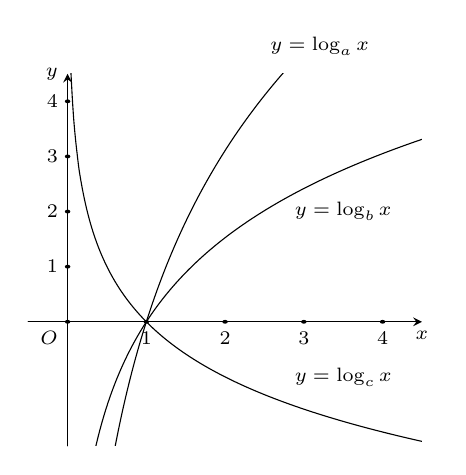
\begin{tikzpicture}[scale=1,>=stealth,font=\scriptsize,line join=round,line cap=round,yscale=.7]
				\draw[->] (-0.5,0)--(4.5,0) node[below] {$x$}; 
				\draw[->] (0,-2.25)--(0,4.5) node[left] {$y$}; 
				\fill (0,0) circle (1pt) node[below  left]{$O$};
				\node at (3.2,5) {$y=\log_a  x$};
				\node at (3.5,2) {$y=\log_b  x$};
				\node at (3.5,-1) {$y=\log_c x$}; 
				\clip (-0.5,-2.25)  rectangle (4.5,4.5);
				\foreach  \x in {1,2,3,4}{\fill (\x,0) circle (1pt) node[below]{$\x$};}
				\foreach \y in {1,2,3,4}{\fill (0,\y) circle (1pt) node[left]{$\y$};} 
				 \draw[domain=0.01:4.5,samples=200,smooth]
					plot (\x,{ln (\x)/ln  (1.25)});
				 \draw[domain=0.01:4.5,samples=200,smooth]
					 plot (\x,{ln (\x)/ln (3.91^(1/3))});
				 \draw[domain=0.01:4.5,samples=200,smooth]
					plot (\x,{ln (\x)/ln  (0.5)});
			\end{tikzpicture}
	\end{center}
	\choiceTF 
		{\True Trong các hàm số $y=\log_a x$, $y=\log_b x$, $y=\log_c x$ (đồ thị trên hình vẽ), có đúng hai hàm số đồng biến trên các  tập xác định của nó}
		{\True $\log_c x > \log_c 2  \Rightarrow x<2$}
		 {$c<b<a$}
		{Đường thẳng $y=3$ cắt trục $Oy$ và cắt đồ  thị các hàm số $y=\log_a x$, $y=\log_b x$ lần lượt tại các điểm $M$, $N$, $P$ sao cho $N$ là trung điểm của $MP$. Khi đó $a^3=2b^3$}
	\loigiai{ 
		\begin{itemchoice}
			\itemch Hàm số $y=\log_a x$, $y=\log_b x$ đồng  biến, $y=\log_c x$ nghịch biến.
			\itemch Hàm $y=\log_c  x$ nghịch biến nên $\log_c x > \log_c 2 \Rightarrow x<2$.
			\itemch Vì $y=\log_a x$, $y=\log_b x$ đồng biến, nên $a>1$, $b>1$.\\ Vì $y=\log_c x$ nghịch biến, nên $0<c<1$. Kẻ đường $y=1$ cắt  các đồ thị, ta thấy hoành độ của giao điểm với $y=\log_a x$ nhỏ hơn của $y=\log_b x$, tức là $a<b$.\\
			 Vậy $c<a<b$.
			 \itemch
			\begin{center}
				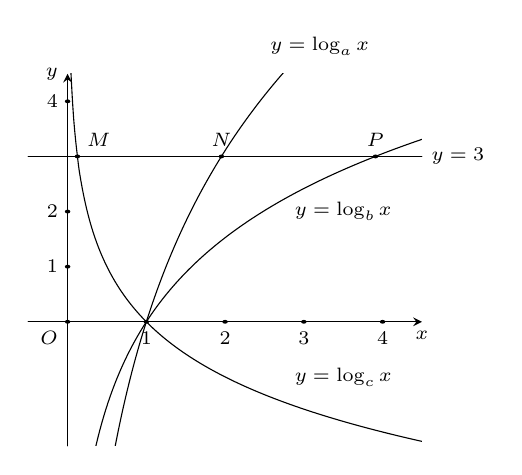
\begin{tikzpicture}[scale=1,>=stealth,font=\scriptsize,line join=round,line cap=round,yscale=.7]
						\draw[->]  (-0.5,0)--(4.5,0) node[below] {$x$};
						\draw[->] (0,-2.25)--(0,4.5) node[left]  {$y$};
						 \fill (0,0) circle (1pt) node[below left]{$O$};
						\node at (3.2,5) {$y=\log_a x$}; 
						\node at (3.5,2) {$y=\log_b x$}; 
						\node at (3.5,-1)  {$y=\log_c x$};
						\draw (-0.5,3)--(4.5,3) node[right]{$y=3$}; 
						\fill ({0.5^3},3) circle (1pt)  node[above right]{$M$}
						({1.25^3},3) circle (1pt) node[above]{$N$} 
						(3.91,3)  circle (1pt) node[above]{$P$};
						\clip (-0.5,-2.25) rectangle (4.5,4.5); 
						 \foreach \x in {1,2,3,4}{\fill (\x,0) circle (1pt) node[below]{$\x$};}
						\foreach \y in {1,2,4}{\fill  (0,\y) circle (1pt) node[left]{$\y$};}
						 \draw[domain=0.01:4.5,samples=200,smooth]
						 plot (\x,{ln (\x)/ln (1.25)});
						\draw[domain=0.01:4.5,samples=200,smooth] 
						plot (\x,{ln  (\x)/ln (3.91^(1/3))});
						\draw[domain=0.01:4.5,samples=200,smooth] 
						plot (\x,{ln (\x)/ln (0.5)}); 
					\end{tikzpicture}
			\end{center}
			Đường thẳng $y=3$ cắt trục $Oy$ và cắt đồ  thị các hàm số $y=\log_a x$, $y=\log_b x$ lần lượt tại các điểm $M(0;3)$, $N(a^3;3)$, $P(b^3;3)$.\\
			Vì $N$ là trung điểm của $MP$ nên \[x_N=\dfrac{x_M+x_P}{2} \Leftrightarrow  a^3=\dfrac{0+b^3}{2} \Leftrightarrow 2a^3=b^3.\]
		\end{itemchoice}
	} 
\end{ex}

% nguồn: Ok_dungsai_lop11_Lan1
\begin{ex}%[1D6V4-2]%[ma:a97a5077]
 Cho phương trình $\log_5\sqrt{x^2-3x+21}=1$ $(*)$  , biết phương trình có hai nghiệm $x_1,x_2$ $\left(x_1<x_2\right)$ . Khi đó:
  \choiceTF
  {\True Phương trình $(*)$ có  chung tập nghiệm với phương trình $x^2-3\rm{x-4=0}$}
  {Tổng  các nghiệm của phương trình $(*)$ bằng $4$}
  {Ba số $x_1,x_2,8$ tạo thành một cấp số cộng} 
  {\True  $\lim\limits_{x\to{x_1}}\left(x-2\right)+\lim\limits_{x\to{x_2}}\left(x-2\right)=-1$}
  \loigiai{
  Điều kiện: $x^2-3\rm{x}+21 > 0$  $\left(**\right)$\\
  $\log_5\sqrt{x^2-3\rm{x}+21}=1$ $\Leftrightarrow $ $\sqrt{x^2-3\rm{x}+21}=5$  $\Rightarrow $ $x^2-3\rm{x-4=0}$ $\Leftrightarrow $ $\hoac{& x=-1\\
   &x=4.}$ \\
  Thay lần  lượt hai giá trị này vào $\left(**\right)$ , ta thấy cả hai giá trị đều thỏa mãn.\\
 Vậy  tập nghiệm của phương trình là $S=\left\{{-1;4}\right\}$ .}
\end{ex}

% nguồn: Ok_dungsai_lop11_Lan1
\begin{ex}%[1D6V4-2]%[ma:bf6a31da]
 Cho bất phương trình $\left(\dfrac{1}{9}\right)^x\ge 27\cdot 3^x$,  có tập nghiệm là $S=(-\infty;b]$. Khi đó
 \choiceTF 
  {\True Bất phương trình có  chung tập nghiệm với $3^{-2x}\ge 3^{3+x}$}
  {\True $A(0;b)$ là giao điểm của đồ thị $y=x^3+2x-1$ với trục tung $Oy$} 
  {\True $\lim\limits_{x\to  -\infty}(3x+2)=-\infty$}
  {$\lim\limits_{x\to b}(3x+2)=2$} 
 \loigiai{ 
   Ta có
  \allowdisplaybreaks 
  \begin{eqnarray*}
   \left(\dfrac{1}{9}\right)^x\ge  27\cdot 3^x&\Leftrightarrow&\left(3^{-2}\right)^{x}\ge 3^3\cdot 3^x\\
   &\Leftrightarrow&3^{-2x}\ge 3^{x+3}\\ 
    &\Leftrightarrow& -2x\ge x+3\\
   &\Leftrightarrow& x\le  -1.
  \end{eqnarray*}
  Bất phương trình có tập nghiệm là  $S=(-\infty;-1]$.
  \begin{itemize}
   \item Ta có 
   \allowdisplaybreaks 
   \begin{eqnarray*}
    3^{-2x}\ge 3^{x+3}&\Leftrightarrow& -2x\ge  x+3\\
    &\Leftrightarrow&  x\le -1.
   \end{eqnarray*}
   \item  Với $x=0$, ta có $y=-1$. Do đó, tọa độ giao điểm của đồ thị hàm số $y=x^3+2x-1$ và trục $Oy$ là $A(0;-1)$.
   \item  $\lim\limits_{x\to -\infty}(3x+2)\lim\limits_{x\to -\infty}x\left(3+\dfrac{2}{x}\right)=-\infty$.
   \item $\lim\limits_{x\to b}(3x+2)=\lim\limits_{x\to  -1}(3x+2)=-3+2=-1$.
  \end{itemize}
  }
\end{ex}

% nguồn: Ok_dungsai_lop11_Lan2
\begin{ex}%[1D6V4-2]%[ma:08589f73]
	 Cho phương trình $\log_2\left(2^{x+1}-2\right)=x+m$.\quad$(1)$
	 \choiceTF
		{Với $m=0$ Phương trình $(1)$ có hai nghiệm phân  biệt}
		{\True Với $m=0$ , gọi $x_0$  là một nghiệm dương của $(1)$ khi đó $3^{2x_0+y}=81$ khi và chỉ khi $y=2$}
		{Phương trình $(1)$ có nghiệm khi  và chỉ khi $m < 2$}
		{\True Giả sử rằng phương trình $(1)$ có nghiệm $x_0$. Khi đó, giá trị nhỏ nhất của $P=2^{x_0}-2^m+2$ bằng  $2\sqrt 2 $}
	 \loigiai{
		\begin{itemchoice}
			\itemch Với $m=0\Rightarrow{\log_2}\left(2^{x+1}-2\right)=x\Leftrightarrow\heva{&x > 0\\&{2^{x+1}}-2=2^x} \Leftrightarrow\heva{&x > 0\\&2^x=2} \Leftrightarrow x=1$ nên $(1)$ có  một nghiệm.
			 \itemch Ta có $x_0=1\Rightarrow {3^{2x_0+y}}=81\Leftrightarrow{3^{2+y}}=3^4\Leftrightarrow 2+y=4\Leftrightarrow y=2$.
			 \itemch Ta có
			\allowdisplaybreaks 
			\begin{eqnarray*}
				&& \log_2\left(2^{x+1}-2\right)=x+m\\ 
				&\Leftrightarrow&\heva{&x > 0\\&2^{x+1}-2=2^{x+m}}7\\ 
				&\Leftrightarrow& \heva{&x > 0\\&2^x\left(2-2^m\right)=2}\\ &\Leftrightarrow& \heva{&x > 0\\&m\ne 1\\&2^x=\dfrac{2}{2-2^m}>  0} \\
				&\Leftrightarrow& \heva{&m\ne 1\\&m < 1} \\ 
				&\Leftrightarrow& m  < 1.
			\end{eqnarray*}
			\itemch $2^{x_0}=\dfrac{2}{2-2^m}\Rightarrow P=\dfrac{2}{2-2^m}+2-2^m\ge 2\sqrt{\dfrac{2}{2-2^m}\cdot \left(2-2^m\right)}=2\sqrt  2 $.\\
			Dấu bằng xảy ra khi và chỉ  khi
			\allowdisplaybreaks 
			\begin{eqnarray*}
				&&2-2^m=\sqrt  2\\
				&\Leftrightarrow& 2^m=2-\sqrt  2\\
				&\Leftrightarrow& m=\log_2\left(2-\sqrt  2\right).
			\end{eqnarray*}
			Vậy  $y_{\min}=2\sqrt 2\Leftrightarrow m=\log_2\left(2-\sqrt 2\right)$.
		\end{itemchoice}
	} 
\end{ex}

% nguồn: Ok_dungsai_lop11_Lan2
\begin{ex}%[1D6V4-2]%[ma:4178ea21]
	Cho phương trình  $\log_5\sqrt{x^2-3x+21}=1$ $(*)$, biết phương trình có hai nghiệm $x_1$, $x_2$ $\left(x_1<x_2\right)$.
	 \choiceTF
		{\True Phương trình  $(*)$ có chung tập nghiệm với phương trình $x^2-3x-4=0$}
		 {Tổng các nghiệm của phương trình $(*)$ bằng $4$}
		{Ba số $x_1$; $x_2$;  $8$ tạo thành một cấp số cộng}
		 {\True $\lim\limits_{x\to{x_1}}\left(x-2\right)+\lim\limits_{x\to{x_2}}\left(x-2\right)=-1$}
	\loigiai{ 
		\begin{itemchoice}
			\itemch Điều kiện:  $x^2-3x+21 > 0$.\quad $(**)$\\
			Ta có $\log_5\sqrt{x^2-3x+21}=1\Rightarrow\sqrt{x^2-3x+21}=5\Rightarrow{x^2}-3x-4=0\Leftrightarrow\hoac{&x=-1\\&x=4.}$\\ 
			Hai nghiệm đều thoả điều kiện  $(**)$ nên suy ra hai phương trình đã cho có cùng tập nghiệm là $S=\{-1;4\}$.
			 \itemch Tổng các nghiệm là $-1+4=3$.
			\itemch $x_1$; $x_2$; $8$ là $-1$; $4$; $8$ không tạo thành cấp số cộng vì $4-(-1)\ne8-4$. 
			\itemch Ta có $\lim\limits_{x\to-1}\left(x-2\right)+\lim\limits_{x\to4}\left(x-2\right)=-1$. 
		\end{itemchoice}
	 }
\end{ex}


%%%%%%%%%%%%%%%% TRẢ LỜI NGẮN %%%%%%%%%%%%%%%%

% nguồn: Ok_TraLoiNgan_Lop11_Lan2
\begin{ex}%[1D6H4-2]%[ma:5e9ae2d0]
	Tổng các nghiệm của phương trình  $2^{x^2 +2x} =8^{2-x} $ bằng
	 \shortans{-5}
	 \loigiai{
		Ta có 
		\begin{eqnarray*}
			&&2^{x^2 +2x} =8^{2-x}\\ 
			&\Leftrightarrow&  2^{x^2 +2x} =2^{3(2-x)} \\
			 &\Leftrightarrow& x^2 +2x=6-3x\\
			&\Leftrightarrow& x^2 +5x-6=0 
		\end{eqnarray*}
	Do đó tổng  các nghiệm của phương trình là $S=-\dfrac{b}{a} =-5$.}
\end{ex}

% nguồn: Ok_TraLoiNgan_Lop11_Lan2
\begin{ex}%[1D6H4-2]%[ma:d37396ad]
	Tổng các nghiệm của  phương trình $3^{x^2 -2x-5} =27$ là
	\shortans{2} 
	\loigiai{ 
		 Ta có
		\begin{eqnarray*}
			3^{x^2 -2x-5} =27  &\Leftrightarrow& 3^{x^2 -2x-5} =3^3 \\
			&\Leftrightarrow&  x^2 -2x-5=3\\
			&\Leftrightarrow  &x^2 -2x-8=0\\
			 &\Leftrightarrow& \hoac{&x=-2\\&x=4.}
		\end{eqnarray*}
	 Tổng các nghiệm của phương trình là $2$.}
\end{ex}

% nguồn: Ok_TraLoiNgan_Lop11_Lan2
\begin{ex}%[1D6H4-2]%[ma:cffa1215]
	Phương trình $\log _2 x+\log  _2 (x-3)=2$ có bao nhiêu nghiệm?
	 \shortans{1}
	\loigiai{ 
		Điều kiện  $\heva{&x>0\\&x-3>0} \Rightarrow x>3$.\\
		Ta có 
		\[\log _2 x+\log _2 (x-3)=2\Leftrightarrow \log _2 \left[x\cdot(x-3)\right]=2\Leftrightarrow x^2 -3x-4=0\Leftrightarrow \hoac{&x=-1\, \,  \, (\text{loại})\\&x=4.}\]
	Vậy phương trình có nghiệm duy  nhất $x=4$.}
\end{ex}

% nguồn: Ok_TraLoiNgan_Lop11_Lan2
\begin{ex}%[1D6H4-2]%[ma:0e3c32c4]
	Tính tổng $T$  tất cả các nghiệm của phương trình $\mathrm{e}^{x^2 -3x} =\dfrac{1}{\mathrm{e}^2} $.
	 \shortans{3}
	 \loigiai{
		 Ta có
		\begin{eqnarray*}
			\mathrm{e}^{x^2 -3x}  =\dfrac{1}{\mathrm{e}^2} &\Leftrightarrow& \mathrm{e}^{x^2 -3x} =\mathrm{e}^{-2}\\
			&  \Leftrightarrow& x^2 -3x=-2\\
			&\Leftrightarrow&  x^2 -3x+2=0\Leftrightarrow \hoac{&x=1\\&x=2.}
		\end{eqnarray*}
	Tập nghiệm của phương trình là $S=\{1;2\}$  nên tổng các nghiệm là $T=3$}
\end{ex}

% nguồn: Ok_TraLoiNgan_Lop11_Lan2
\begin{ex}%[1D6H4-2]%[ma:4e4378cc]
	Tổng các nghiệm thực của phương trình $\log _2  (x+1)=2\log _4 (x^2 -1)$ bằng
	 \shortans{2}
	 \loigiai{
		Điều kiện $\heva{&x+1>0\\&x^2 -1>0} \Leftrightarrow x>1$.\\ 
		Ta  có
		\begin{eqnarray*}
			\log _2 (x+1)=2\log _4 (x^2 -1)&\Leftrightarrow& \log _2  (x+1)=\log _2 (x^2 -1)\\
			&\Leftrightarrow& x+1=x^2 -1\\ 
			&\Leftrightarrow & x^2 -x-2=0\Leftrightarrow \hoac{&x=2\\&x=-1.} 
		\end{eqnarray*}
	So điều kiện ta nhận $x=2$. Vậy tổng các nghiệm thực của phương trình là  $2$.}
\end{ex}

% nguồn: Ok_TraLoiNgan_Lop11_Lan2
\begin{ex}%[1D6H4-2]%[ma:c10283c2]
	Tổng các nghiệm của phương trình $\log (x^2 +1)=\log (2x^2  -3)$ là
	\shortans{0} 
	 \loigiai{
		Điều kiện $\heva{&x^2  +1>0\\&2x^2 -3>0} \Leftrightarrow x^2 >\dfrac{3}{2} \Leftrightarrow \hoac{&x<-\dfrac{\sqrt{6}}{2}\\&x>\dfrac{\sqrt{6}}{2}.} $\\
		Ta có $\log (x^2 +1)=\log (2x^2 -3)$ $\Leftrightarrow  x^2 +1=2x^2 -3\Leftrightarrow x^2 =4\Leftrightarrow x=\pm 2$.\\
	Do vậy tổng các nghiệm của phương trình  bằng $x_1+x_2=-2+2=0$.}
\end{ex}

% nguồn: Ok_TraLoiNgan_Lop11_Lan2
\begin{ex}%[1D6H4-2]%[ma:7672474a]
	Tích các nghiệm thực  phân biệt của phương trình $2^{x^2 +x} =1$ là
	 \shortans{0}
	 \loigiai{
		Ta có $2^{x^2 -x} =1\Leftrightarrow x^2  -x=0\Leftrightarrow \hoac{&x=0\\&x=1.}$\\
	Vậy tích các nghiệm là $0$.} 
\end{ex}

% nguồn: Ok_TraLoiNgan_Lop11_Lan2
\begin{ex}%[1D6H4-2]%[ma:cac5fc09]
	Tổng các  nghiệm của phương trình $\log _4 x^2 -\log _2 6=0$ là
	 \shortans{0}
	 \loigiai{
		Điều kiện $x\ne 0$. Ta  có\\
		$\log _4 x^2 -\log _2 6=0\Leftrightarrow \log _2 \left|  x\right| =\log _2 6\Leftrightarrow \left| x\right| =6\Leftrightarrow \hoac{&x=6\\&x=-6.} $\\
	Vậy tổng  các nghiệm phương trình đã cho bằng $0$.}
\end{ex}

% nguồn: Ok_TraLoiNgan_Lop11_Lan2
\begin{ex}%[1D6H4-2]%[ma:04bc0ce6]
	Số nghiệm của phương trình $\log _3  (x+1)=\log _{\tfrac{1}{3}} (x+4)$ là
	 \shortans{1}
	 \loigiai{
		Điều  kiện $x>-1$. Ta có
		\begin{eqnarray*}
			&&\log _3 (x+1)=\log _{\tfrac{1}{3}}  (x+4)\\
			 &\Leftrightarrow& \log _3 (x+1)=\log _3 (x+4)^{-1}\\
			 &\Leftrightarrow& x+1=(x+4)^{-1}\\
			&\Leftrightarrow& x+1=\dfrac{1}{x+4} \\ 
			&\Leftrightarrow& x^2 +5x+3=0\Leftrightarrow  \hoac{&x=\dfrac{-5+\sqrt{13}}{2}\\&x=\dfrac{-5-\sqrt{13}}{2}.}
		\end{eqnarray*}
		 Đối chiếu với điều kiện, chỉ có nghiệm $x=\dfrac{-5+\sqrt{13}}{2} $ thỏa mãn.\\
	Vậy phương trình đã  cho có $1$ nghiệm.}
\end{ex}

% nguồn: Ok_TraLoiNgan_Lop11_Lan2
\begin{ex}%[1D6H4-2]%[ma:d66cbed8]
	Số nghiệm của phương trình $\log _3 (x^2 +4x)+\log  _{\tfrac{1}{3}} (2x+3)=0$ là
	\shortans{1} 
	 \loigiai{
		Điều kiện $\heva{&x^2 +4x>0\\&2x+3>0} \Leftrightarrow \heva{&\hoac{&x>0\\&x<-4}\\&x>-\dfrac{3}{2}} \Leftrightarrow  x>0$.\\
		 Ta có
		\begin{eqnarray*}
			&&\log _3 (x^2 +4x)+\log _{\tfrac{1}{3}}  (2x+3)=0\\
			&\Leftrightarrow&  \log _3 (x^2 +4x)=\log _3 (2x+3)\\
			 &\Leftrightarrow& x^2 +4x=2x+3b\\
			&\Leftrightarrow& x^2  +2x-3=0 \Leftrightarrow \hoac{&x=1\\&x=-3.}
		\end{eqnarray*}
	Kết hợp điều kiện ta được $x=1$. Vậy phương trình đã cho có $1$  nghiệm.}
\end{ex}

% nguồn: Ok_TraLoiNgan_Lop11_Lan2
\begin{ex}%[1D6H4-2]%[ma:12e8def1]
	Phương trình $\log  _3 (4x-2)-\log _3 (x^2 +1)=0$ có hai nghiệm $x_1$, $x_2$ ($x_1<x_2$). Tính $2x_1 +x_2 $.
	 \shortans{5}
	 \loigiai{
		Điều  kiện $x>\dfrac{1}{2} $. Ta có
		\begin{eqnarray*}
			\log _3 (4x-2)-\log _3 (x^2  +1)=0&\Leftrightarrow& \log_3 (4x-2)=\log _3 (x^2 +1)\\
			&\Leftrightarrow& 4x-2=x^2  +1\\
			 &\Leftrightarrow& x^2 -4x+3=0\Leftrightarrow \hoac{&x=1\\&x=3.}
		\end{eqnarray*}
		 Suy ra $x_1=1$, $x_2=3$. Vậy $2x_1 +x_2 =5$
	} 
\end{ex}

% nguồn: Ok_TraLoiNgan_Lop11_Lan2
\begin{ex}%[1D6H4-2]%[ma:362006f7]
	Số nghiệm của phương trình $\log  (x^2 +4)=\log 4x$ là
	\shortans{1} 
	 \loigiai{
		Điều kiện $\heva{&x^2 +4>0\\&4x>0} \Leftrightarrow  x>0$.\\
		 Với điều kiện trên ta có
		\[\log (x^2 +4)=\log 4x \Leftrightarrow x^2 +4=4x\Leftrightarrow x^2 -4x+4=0\Leftrightarrow x=2.\] 
	Vậy phương  trình có $1$ nghiệm.}
\end{ex}

% nguồn: Ok_TraLoiNgan_Lop11_Lan2
\begin{ex}%[1D6H4-2]%[ma:1bca0ec7]
	Cho số thực $x$  thỏa mãn $\log _2 (\log _8 x)=\log _8 (\log _2 x)$. Tính giá trị $P=(\log _2 x)^4 $.
	\shortans{729} 
	\loigiai{ 
		Điều kiện $x>1$. Ta  có
		\begin{eqnarray*}
			&&\log _2 (\log _8 x)=\log _8 (\log _2 x)\\ 
			&\Leftrightarrow& \log _2 (\log _8 x)=\dfrac{1}{3} \log  _2 (\log _2 x)\\
			 &\Leftrightarrow& 3\log _2 (\log _8 x)=\log _2 (\log _2 x)\\
			&\Leftrightarrow& \log _2 (\log _8 x)^3 =\log  _2 (\log _2 x)\\
			&\Leftrightarrow& (\log _8  x)^3 =\log _2 x\\
			&\Leftrightarrow& \dfrac{1}{27} \log _2^3 x-\log _2  x=0\\
			&\Leftrightarrow& \hoac{&\log _2 x=0\, \, \, (\text{loại})\\&\log _2 x=3\sqrt{3}\\&\log  _2 x=-3\sqrt{3}. \, \, \, (\text{loại})}
		\end{eqnarray*}
	Vậy $P=(\log _2 x)^4 =(3\sqrt{3})^4 =729$.} 
\end{ex}

% nguồn: Ok_TraLoiNgan_Lop11_Lan2
\begin{ex}%[1D6H4-2]%[ma:660ff35e]
	Tổng tất cả các nghiệm của phương  trình $\log _2 (x-1)+\log _2 x=1+\log _2 (3x-5)$ bằng
	 \shortans{7}
	\loigiai{ 
		Điều kiện $x>\dfrac{5}{3}  $. Ta có
		\begin{eqnarray*}
			&&\log  _2 (x-1)+\log _2 x=1+\log _2 (3x-5)\\
			&\Leftrightarrow& \log _2 (x-1)x=\log _2 (2(3x-5))\\ 
			 &\Leftrightarrow& x^2 -x=6x-10\\
			&\Leftrightarrow& x^2 -7x+10=0\Leftrightarrow  \hoac{&x=2\\&x=5.}
		\end{eqnarray*}
	Vậy tổng các nghiệm bằng $7$.} 
\end{ex}

% nguồn: Ok_TraLoiNgan_Lop11_Lan2
\begin{ex}%[1D6H4-2]%[ma:2f5e1094]
	Phương trình $\log _x 2+\log _2 x=\dfrac{5}{2} $ có hai nghiệm $x_1 ,x_2 (x_1 <x_2)$. Khi đó tổng $x_1^2 +x_2 $ bằng 
	 \shortans{6}
	 \loigiai{
		 Điều kiện $x>0$, $x\ne 1$.
		Ta  có
		\begin{eqnarray*}
			\log _x 2+\log  _2 x=\dfrac{5}{2} &\Leftrightarrow& \dfrac{1}{\log _2 x} +\log _2 x=\dfrac{5}{2} \\
			&\Leftrightarrow& (\log _2 x)^2 -\dfrac{5}{2}  \log _2 x+1=0\\
			&\Leftrightarrow& \hoac{&\log _2  x=2\\&\log _2 x=\dfrac{1}{2}} \\ &\Leftrightarrow& \hoac{&x=4\\&x=\sqrt{2}}
		\end{eqnarray*}
	Suy ra $x_1 =\sqrt{2}  ,\, x_2 =4$. Vậy $x_1^2 +x_2 =6$.}
\end{ex}

% nguồn: Ok_TraLoiNgan_Lop11_Lan2
\begin{ex}%[1D6H4-2]%[ma:9301ca49]
	Số nghiệm của phương trình $\log _3  (x^2 -6)=\log _3 (x-2)+1$ là
	\shortans{1} 
	\loigiai{ 
		Điều kiện $\heva{&x^2 -6>0\\&x-2>0} \Leftrightarrow \heva{&x\in (-\infty \,;\, -\sqrt{6})\cup  (\sqrt{6} \,;\, +\infty)\\&x>2} \Leftrightarrow x\in (\sqrt{6} \,;\, +\infty)$.\\
		Ta có 
		\begin{eqnarray*}
			&& \log _3 (x^2 -6)=\log _3 (x-2)+1\\ 
			&\Leftrightarrow& \log _3 (x^2  -6)=\log _3 (x-2)+\log _3 3\\
			&\Leftrightarrow& \log _3 (x^2 -6)=\log _3  (3x-6)\\
			&\Leftrightarrow&  x^2 -6=3x-6 \\
			&\Leftrightarrow& \hoac{&x=0\, \, (\text{loại})\\&x=3} \Leftrightarrow  x=3.
		\end{eqnarray*}
		Vậy phương trình có $1$ nghiệm. 
	 }
\end{ex}

% nguồn: Ok_TraLoiNgan_Lop11_Lan2
\begin{ex}%[1D6H4-2]%[ma:77932717]
	 Tổng tất cả các nghiệm thực của phương trình $\log _3 (x^2 -5x+1)=2$ bằng
	\shortans{5} 
	\loigiai{ 
		Điều kiện $ x^2 -5x+1>0 \Leftrightarrow \hoac{&x<\dfrac{5-\sqrt{21}}{2}\\&  x>\dfrac{5+\sqrt{21}}{2}.}$\\
		 Ta có
		\[\log _3 (x^2  -5x+1)=2\Leftrightarrow x^2 -5x+1=9\Leftrightarrow x^2 -5x-8=0 \Leftrightarrow \hoac{&x=\dfrac{5-\sqrt{57}}{2}\\& x=\dfrac{5+\sqrt{57}}{2}.}\]
	Suy ra tổng các nghiệm là  $5$.}
\end{ex}

% nguồn: Ok_TraLoiNgan_Lop11_Lan2
\begin{ex}%[1D6H4-2]%[ma:4ea24881]
	Gọi $x_0 $  nghiệm của phương trình: $\log _4 (\log _2 x)+\log _2 (\log _4 x)=2$. Giá trị của biểu thức $P=x_0^2 -3x_0 $ bằng
	 \shortans{208}
	\loigiai{ 
		Điều  kiện $\heva{&x>0\\&\log _2 x>0} \Leftrightarrow x>1$. Ta có
		\begin{eqnarray*}
			\log _4 (\log _2 x)+\log _2 (\log _4 x)=2&\Leftrightarrow& \dfrac{1}{2}  \log _2 (\log _2 x)+\log _2 \left(\dfrac{1}{2} \log _2 x\right)=2\\
			&\Leftrightarrow& \dfrac{1}{2} \log _2 (\log _2 x)+\log _2 \dfrac{1}{2} +\log  _2 (\log _2 x)=2\\
			&\Leftrightarrow& \dfrac{3}{2} \log _2 (\log  _2 x)=3\\
			&\Leftrightarrow& \log _2  (\log _2 x)=2\\
			&\Leftrightarrow& \log  _2 x=4\Leftrightarrow x=16.
		\end{eqnarray*}
	 Vậy $P=x_0^2 -3x_0 =16^2 -3\cdot 16=208$.}
\end{ex}

% nguồn: Ok_TraLoiNgan_Lop11_Lan1
\begin{ex}%[1D6V4-2]%[ma:02e069b3]
	Cho các hàm số $y=3^{3x+1}$ và $y=9^x$ có đồ thị  lần lượt là $(C_1)$ và $(C_2)$. Gọi $A$ là giao điểm của $(C_1)$ và $(C_2)$. Gọi $B$, $C$ lần lượt là giao điểm của trục $Oy$ với $(C_1)$ và $(C_2)$. Diện tích của tam giác $ABC$ bằng bao nhiêu?
	\shortans{1} 
	 \loigiai{
	Tọa độ điểm $A$ là nghiệm hệ phương trình 
	$$\heva{&y=3^{3x+1}\\&y=9^x}\Leftrightarrow \heva{&3^{3x+1}=9^x\\&y=9^x}\Leftrightarrow\heva{&x=-1\\&y=\dfrac{1}{9}.}$$ 
	Do đó $A\left(-1;\dfrac{1}{9}\right)$.\\ 
	$B$, $C$ lần lượt là giao điểm của trục $Oy$ với $(C_1)$ và $(C_2)$ nên ta có $B(0;3)$,  $C(0;1)$.\\
	 Diện tích tam giác $ABC$ là $S_{ABC}=\dfrac{1}{2}BC\cdot \mathrm{d}(A,BC)=\dfrac{1}{2}\cdot 2\cdot 1=1$.
	 }
\end{ex}

% nguồn: Ok_TraLoiNgan_Lop11_Lan2
\begin{ex}%[1D6V4-2]%[ma:3ffad98c]
	Phương trình $\dfrac{1}{2} \log _{\sqrt{3}} (x+3)+\dfrac{1}{2} \log _9 (x-1)^4 =2\log _9 (4x)$ có bao nhiêu nghiệm thực phân biệt? 
	 \shortans{2}
	 \loigiai{
		Điều kiện $\heva{&x>0\\&x\ne 1.} $ \\ 
		Ta  có
		\begin{eqnarray*}
			&&\dfrac{1}{2} \log _{\sqrt{3}} (x+3)+\dfrac{1}{2} \log _9 (x-1)^4  =2\log _9 (4x)\\
			 &\Leftrightarrow& \log _3 (x+3)+\log _3 \left| x-1\right| =\log _3 (4x)\\
			&\Leftrightarrow& (x+3)\left|  x-1\right| =4x\\
			&\Leftrightarrow& \hoac{&\heva{&x>1\\&x^2 -2x-3=0}\\&\heva{&0<x<1\\&x^2  +6x-3=0}} \\
			&\Leftrightarrow& \hoac{&\heva{&x>1\\&x=3\, \, \, (\text{nhận})\\&x=-1\, \, \, (\text{loại})}\\&\heva{&0<x<1\\&x=-3+2\sqrt{3} \, \, \,  (\text{nhận})\\&x=-3-2\sqrt{3} \, \, \, (\text{loại})}} \\
			 &\Leftrightarrow& \hoac{&x=3\\&x=-3+2\sqrt{2}.}
		\end{eqnarray*}
		Vậy phương trình có $2$ nghiệm  thực phân biệt.
	} 
\end{ex}


%%%%%%%%%%%%%%%% TỰ LUẬN %%%%%%%%%%%%%%%%

% nguồn: Ok_TuanLuan_Toan11_Lan1
\begin{bt}%[1D6N4-2]%[ma:c56921c1]
	Giải các  phương trình sau
	\begin{enumerate}
		 \item $3^{x^2-2x-3}=3^{x+1}$.
	\loigiai{Ta có  $3^{x^2-2x-3}=3^{x+1}\Leftrightarrow x^2-2x-3=x+1\Leftrightarrow x^2-3x-4=0\Leftrightarrow\hoac{&x=-1\\&x=4.}$}
		\item  $\log_3(x-1)=2$.
	\loigiai{Ta có $\log_3(x-1)=2\Leftrightarrow x-1=3^2=9\Leftrightarrow x=10$.} 
	\end{enumerate}
\end{bt}

% nguồn: Ok_TuanLuan_Toan11_Lan1
\begin{bt}%[1D6N4-2]%[ma:e544cb69]
	Giải phương trình $\log _2 x+\log _2(x-3)=2$. 
	\loigiai{Điều kiện  $x>3$.\\
		Ta có \begin{eqnarray*}
		&  & \log_2 x+\log_2(x-3)=2\\
		&\Leftrightarrow &  \log_2x(x-3)=2\\
		&\Leftrightarrow  & x^2-3x=2^2\\
		&\Leftrightarrow  & x^2-3x-4=0\\
		&\Leftrightarrow &  \hoac{& x=-1\,\text{(loại)}\\ & x=4.}
	\end{eqnarray*}
	Vậy  phương trình có nghiệm $x=4$.
 }
\end{bt}

% nguồn: Ok_TuanLuan_Toan11_Lan1
\begin{bt}%[1D6N4-2]%[ma:e6cc53a1]
	 Giải các phương trình sau
	\begin{listEX}[2]
		\item $2^{4  x+5}-\dfrac{1}{8}=0$;
		\item $\log _{4}(x-2)=2$; 
		 \item $5^{2 x+1}=\left(\dfrac{1}{125}\right)^{x}$;
		 \item $\log _{3}(x+4)+2 \log _{9}(14-x)=4$.
	\end{listEX}
	\loigiai{ 
		\begin{listEX}[1]
			\item $2^{4  x+5}-\dfrac{1}{8}=0\Leftrightarrow 2^{4 x+5}=2^{-3} \Leftrightarrow 4x+5 = -3\Leftrightarrow x=-3$.\\
			Vậy tập nghiệm  $S=\{-3\}$.
			\item $\log  _{4}(x-2)=2\,\,\,$(1), điều kiện $x-2 >0 \Leftrightarrow x>2$.\\
			Phương trình (1) $\Leftrightarrow x-2 =  4^2 \Leftrightarrow x=18$ (thỏa mãn).\\
			Vậy tập nghiệm $S=\{18\}$. 
			\item $5^{2 x+1}=\left(\dfrac{1}{125}\right)^{x} \Leftrightarrow 5^{2 x+1}=5^{-3x} \Leftrightarrow 2x+1=-3x \Leftrightarrow x=-\dfrac{1}{5}$.\\ 
			Vậy tập nghiệm  $S=\left\{-\dfrac{1}{5}\right\}$.
			 \item $\log _{3}(x+4)+2 \log _{9}(14-x)=4\,\,\,$(2).\\
			Điều kiện $\heva{&x+4>0\\&14-x>0}\Leftrightarrow\heva{&x>-4\\&x<14}\Leftrightarrow -4<x<14.$\\ 
			Phương trình (2) tương  đương với
			\begin{align*}
				 &\log _{3}(x+4)+ \log _{3}(14-x)=4\\
				 \Leftrightarrow& \log _{3}(x+4)(14-x)=4\\
				 \Leftrightarrow& (x+4)(14-x)=81\\
				\Leftrightarrow& -x^2 +10x +64 =  81\\
				\Leftrightarrow& x^2 -10x +  17=0\\
				\Leftrightarrow& \hoac{&x=5-2\sqrt{2}\\&x=5+2\sqrt{2}} \,\,\text{(thỏa  điều kiện)}.
			\end{align*}
			Vậy tập  nghiệm $S=\left\{5-2\sqrt{2},5+2\sqrt{2}\right\}$.
		\end{listEX}
	 }
\end{bt}

% nguồn: Ok_TuanLuan_Toan11_Lan2
\begin{ex}%[1D6N4-2]%[ma:b13a578f]
	Giải các phương  trình sau
	\begin{enumerate}
		 \item $3^{x^2-2x-3}=3^{x+1}$.
	\loigiai{Ta có $3^{x^2-2x-3}=3^{x+1}\Leftrightarrow  x^2-2x-3=x+1\Leftrightarrow x^2-3x-4=0\Leftrightarrow\hoac{&x=-1\\&x=4.}$}
		 \item $\log_3(x-1)=2$.
	\loigiai{Ta có $\log_3(x-1)=2\Leftrightarrow  x-1=3^2=9\Leftrightarrow x=10$.}
	\end{enumerate}
\end{ex}

% nguồn: Ok_TuanLuan_Toan11_Lan2
\begin{ex}%[1D6N4-2]%[ma:8e4008ee]
	Giải phương trình $\log  _2 x+\log _2(x-3)=2$.
	\loigiai{Điều kiện  $x>3$.\\
		Ta có \begin{eqnarray*}
		& & \log_2 x+\log_2(x-3)=2\\ 
		 &\Leftrightarrow & \log_2x(x-3)=2\\
		&\Leftrightarrow & x^2-3x=2^2\\ 
		 &\Leftrightarrow & x^2-3x-4=0\\
		 &\Leftrightarrow & \hoac{& x=-1\,\text{(loại)}\\ & x=4.}
	\end{eqnarray*}
	Vậy  phương trình có nghiệm $x=4$.
 }
\end{ex}

% nguồn: Ok_TuanLuan_Toan11_Lan2
\begin{ex}%[1D6N4-2]%[ma:440b685d]
	Giải các phương trình  sau
	\begin{listEX}[2]
		\item $2^{4  x+5}-\dfrac{1}{8}=0$;
		\item  $\log _{4}(x-2)=2$;
		\item $5^{2 x+1}=\left(\dfrac{1}{125}\right)^{x}$; 
		\item $\log  _{3}(x+4)+2 \log _{9}(14-x)=4$.
	\end{listEX}
	 \loigiai{
		\begin{listEX}[1]
			\item $2^{4 x+5}-\dfrac{1}{8}=0\Leftrightarrow 2^{4 x+5}=2^{-3} \Leftrightarrow  4x+5 = -3\Leftrightarrow x=-3$.\\
			Vậy tập nghiệm  $S=\{-3\}$.
			\item $\log _{4}(x-2)=2\,\,\,$(1), điều kiện  $x-2 >0 \Leftrightarrow x>2$.\\
			Phương trình (1) $\Leftrightarrow x-2  = 4^2 \Leftrightarrow x=18$ (thỏa mãn).\\
			Vậy tập  nghiệm $S=\{18\}$.
			\item $5^{2 x+1}=\left(\dfrac{1}{125}\right)^{x} \Leftrightarrow 5^{2  x+1}=5^{-3x} \Leftrightarrow 2x+1=-3x \Leftrightarrow x=-\dfrac{1}{5}$.\\
			Vậy tập nghiệm $S=\left\{-\dfrac{1}{5}\right\}$. 
			\item $\log  _{3}(x+4)+2 \log _{9}(14-x)=4\,\,\,$(2).\\
			Điều kiện  $\heva{&x+4>0\\&14-x>0}\Leftrightarrow\heva{&x>-4\\&x<14}\Leftrightarrow -4<x<14.$\\
			Phương trình (2) tương đương  với
			\begin{align*}
				&\log _{3}(x+4)+ \log _{3}(14-x)=4\\ 
				 \Leftrightarrow& \log _{3}(x+4)(14-x)=4\\
				\Leftrightarrow&  (x+4)(14-x)=81\\
				\Leftrightarrow&  -x^2 +10x +64 = 81\\
				\Leftrightarrow& x^2  -10x + 17=0\\
				\Leftrightarrow& \hoac{&x=5-2\sqrt{2}\\&x=5+2\sqrt{2}}  \,\,\text{(thỏa điều kiện)}.
			\end{align*}
			Vậy tập  nghiệm $S=\left\{5-2\sqrt{2},5+2\sqrt{2}\right\}$.
		\end{listEX}
	 }
\end{ex}

% nguồn: Ok_TuanLuan_Toan11_Lan2
\begin{ex}%[1D6N4-2]%[ma:249a3bd3]
	 Giải phương trình $\log_3x=4$.
	 \loigiai{
		Điều kiện  $x > 0$.\\
		Ta có $\log_3x=4\Leftrightarrow x=3^4\Leftrightarrow  x=81$.\\
		Vậy nghiệm của phương trình là  $x=81$.
	 }
\end{ex}

% nguồn: Ok_TuanLuan_Toan11_Lan2
\begin{ex}%[1D6N4-2]%[ma:fbf5baa0]
	Giải phương trình $\log_2\left(2x-2\right)=3$. 
	\loigiai{ 
		 Điều kiện $2x-2> 0\Leftrightarrow x > 1$.\\
		Ta có  $\log_2\left(2x-2\right)=3\Leftrightarrow 2x-2=8\Leftrightarrow 2x=10\Leftrightarrow x=5$.\\
		Vậy nghiệm của phương trình là $x=5$. 
	 }
\end{ex}

% nguồn: Ok_TuanLuan_Toan11_Lan2
\begin{ex}%[1D6N4-2]%[ma:f21e0e64]
	Giải phương trình $3^{x-1}  =9$.
	 \loigiai{
		Ta có $3^{x-1}  =9\Leftrightarrow 3^{x-1} =3^{2} \Leftrightarrow x=3$.
	} 
\end{ex}

% nguồn: Ok_TuanLuan_Toan11_Lan1
\begin{bt}%[1D6H4-2]%[ma:e58c15b8]
	Giải các phương  trình sau
	\begin{listEX}[2]
		 \item $3^{x^2+9 x-7}=27$;
		\item $\log_5\left(3  x^2-8 x+4\right)=\log_5(5 x-6)$.
	\end{listEX}
	\loigiai{ 
		\begin{listEX}[1]
			\item Ta có  \allowdisplaybreaks \vspace*{-0.5cm}
			\begin{eqnarray*}
				& & 3^{x^2+9  x-7}=27 \\
				 & \Leftrightarrow & 3^{x^2+9 x-7}=3^3\\
				& \Leftrightarrow & x^2+9  x-7=3\\
				&  \Leftrightarrow & x^2+9 x-10=0 \\
				 & \Leftrightarrow & \hoac{&x=1 \\&x=-10.}
			\end{eqnarray*}
			Vậy tập nghiệm  của phương trình $S=\{-10;1\}$.
			 \item Ta có \allowdisplaybreaks \vspace*{-0.5cm}
			\begin{eqnarray*}
				&  & \log_5\left(3 x^2-8 x+4\right)=\log_5(5 x-6) \\
				& \Leftrightarrow &\heva{&5x-6 >0 \\&3 x^2-8  x+4=5x-6}\\
				& \Leftrightarrow &\heva{&x>\dfrac{6}{5} \\&3 x^2-13  x+10=0}\\
				 & \Leftrightarrow &\heva{&x>\dfrac{6}{5} \\&3 x^2-13 x+10=0}\\
				& \Leftrightarrow &\hoac{&x>\dfrac{6}{5} \\&x=1 \text{ hoặc } x=\dfrac{10}{3}}  \Leftrightarrow x=\dfrac{10}{3}.
			\end{eqnarray*}
			Vậy tập nghiệm của  phương trình $S=\left\{\dfrac{10}{3}\right\}$.
		\end{listEX}
	 }
\end{bt}

% nguồn: Ok_TuanLuan_Toan11_Lan1
\begin{bt}%[1D6H4-2]%[ma:e8cec248]
	Biến  đổi các phương trình sau với phép đặt cho trước.
	\begin{multicols}{2}
		\begin{enumerate}
			\item $4^x-3\cdot  2^{x+1}+2=0$, khi đặt $t=2^x$;
			\item $2^{2x+1}-2^{x-1}-1=0$, khi đặt $h=2^x$; 
			\item  $9^{x+1}-3^{x+1}-30=0$, khi đặt $u=3^x$;
			\item $5^{2x}-3\cdot 5^{x+2}+32=0$, khi  đặt $m=5^x$.
		\end{enumerate}
	\end{multicols}
	\loigiai{ 
		\begin{enumerate}
			\item Ta có $4^x-3\cdot 2^{x+1}+2=0 \Leftrightarrow  \left(2^x\right)^2-6\cdot 2^x+2=0$.\\
			Đặt $t=2^x$, phương trình đã  cho trở thành $t^2-6t+2=0$.
			\item  Ta có $2^{2x+1}-2^{x-1}-1=0 \Leftrightarrow 2\cdot \left(2^x\right)^2-\dfrac{2^x}{2}-1=0$.\\
			Đặt $h=2^x$, phương trình đã cho trở thành $2h^2-\dfrac{1}{2}h-1=0$. 
			\item Ta có $9^{x+1}-3^{x+1}-30=0  \Leftrightarrow 9\cdot \left(3^x\right)^2-3\cdot 3^x-30=0$.\\
			Đặt $u=3^x$, phương trình đã cho trở  thành $9u^2-3u-30=0$.
			\item Ta có $5^{2x}-3\cdot 5^{x+2}+32=0  \Leftrightarrow \left(5^x\right)^2-3\cdot 5^x \cdot 5^2+32=0 \Leftrightarrow \left(5^x\right)^2-75\cdot 5^x+32=0$.\\
			Đặt $m=5^x$, phương trình đã cho trở thành  $m^2-75m+32=0$.
		\end{enumerate}
	 }
\end{bt}

% nguồn: Ok_TuanLuan_Toan11_Lan1
\begin{bt}%[1D6H4-2]%[ma:5451ea73]
	Giải phương  trình sau $2^{x^2-x+8}=4^{1-3x}$.
	 \loigiai{
		\begin{eqnarray*}
			& &  2^{x^2-x+8}=4^{1-3x}\\
			 &\Leftrightarrow & 2^{x^2-x+8}=2^{2\left(1-3x\right)}\\
			& \Leftrightarrow & x^2-x+8=2-6x\\ 
			& \Leftrightarrow &  x^2+5x+6=0\\
			& \Leftrightarrow & \hoac{&x=-2\\&x=-3.} 
		\end{eqnarray*}
	 }
\end{bt}

% nguồn: Ok_TuanLuan_Toan11_Lan1
\begin{bt}%[1D6H4-2]%[ma:85464df2]
	Giải các  phương trình sau
	\begin{multicols}{2}
		\begin{enumerate}
			\item $2^{x+1}=8^{x}$; 
			\item $3^{4^x}=4^{3^x}$; 
			\item  $5^{2x+1}=\left(\dfrac{1}{125}\right)^{x+2}$;
			\item  $2^{x-1}=5^{x^2+2x-3}$;
			\item  $\left(2+\sqrt{3}\right)^{-2x}=\left(2-\sqrt{3}\right)^{x^2}$;
			\item $2^x\cdot  5^x=0{,}2\cdot \left(10^{x-1}\right)^5$.
		\end{enumerate}
	\end{multicols}
	 \loigiai{
		\begin{enumerate}
			\item Ta có $2^{x+1}=8^{x} \Leftrightarrow  x+1=x\log_2 8 \Leftrightarrow x+1=3x \Leftrightarrow x=\dfrac{1}{2}$.\\
			Vậy phương trình  có một nghiệm $x=\dfrac{1}{2}$.
			\item Ta  có
			\begin{eqnarray*}
				&&3^{4^x}=4^{3^x}\\ 
				&\Leftrightarrow& 4^x=3^x\cdot \log_3 4 \\ 
				&\Leftrightarrow& x=\log_4  \left(3^x\cdot \log_3 4\right) \\
				&\Leftrightarrow& x=x\cdot \log_4 3+\log_4\left(\log_3  4\right)\\
				&\Leftrightarrow& x=\dfrac{\log_4\left(\log_3  4\right)}{1-\log_4 3}.
			\end{eqnarray*}
			Vậy phương trình  có một nghiệm $x=\dfrac{\log_4\left(\log_3 4\right)}{1-\log_4 3}$.
			\item Ta có $5^{2x+1}=\left(\dfrac{1}{125}\right)^{x+2} \Leftrightarrow 2x+1=(x+2)\log_5 \dfrac{1}{125}\Leftrightarrow  2x+1=-3x-6\Leftrightarrow x=-\dfrac{7}{5}$.\\
			Vậy phương trình  có một nghiệm $x=-\dfrac{7}{5}$.
			 \item Ta có
			\begin{eqnarray*}
				&&2^{x-1}=5^{x^2+2x-3}\\ 
				&\Leftrightarrow& \log_5 2^{x-1}=\log_5  5^{x^2+2x-3} \\
				 &\Leftrightarrow& (x-1)\log_5 2=x^2+2x-3 \\
				 &\Leftrightarrow& x^2+(2-\log_5 2)x+(\log_5 2 -3)=0 \\
				 &\Leftrightarrow& \hoac{&x=1\\&x=-3+\log_5 2.}
			\end{eqnarray*}
			Vậy  phương trình có hai nghiệm $x=1$, $x=-3+\log_5 2$.
			 \item
			Ta có $(2+\sqrt{3})(2-\sqrt{3})=1  \Rightarrow 2-\sqrt{3}=\dfrac{1}{2+\sqrt{3}}=(2+\sqrt{3})^{-1}$.\\
			 Do đó
			\begin{eqnarray*}
				&&\left(2+\sqrt{3}\right)^{-2x}=\left(2-\sqrt{3}\right)^{x^2} \\ &\Leftrightarrow& -2x=x^2\log_{2+\sqrt{3}} (2-\sqrt{3})  \\
				&\Leftrightarrow& 2x=x^2  \\
				 &\Leftrightarrow& \hoac{&x=0\\&x=2.}\\
			\end{eqnarray*}
			Vậy phương trình có hai  nghiệm $x=0$, $x=2$.
			\item Ta  có
			\begin{eqnarray*}
				&&2^x\cdot 5^x=0{,}2\cdot \left(10^{x-1}\right)^5  \\
				 &\Leftrightarrow& 10^x=0{,}2\cdot 10^{5x-5}\\
				 &\Leftrightarrow& x=\log 0{,}2 +5x-5\\
				&\Leftrightarrow& 4x=6-\log  2\\
				&\Leftrightarrow& x=\dfrac{3}{2}-\dfrac{1}{4}\log 2. 
			\end{eqnarray*}
			Vậy phương trình có một nghiệm $x=\dfrac{3}{2}-\dfrac{1}{4}\log 2$. 
		\end{enumerate}
	 }
\end{bt}

% nguồn: Ok_TuanLuan_Toan11_Lan1
\begin{bt}%[1D6H4-2]%[ma:694e96a7]
	Giải các phương trình  sau
	\begin{enumEX}{3}
		\item  $3^x=4$
		 \item $8^x=4$
		 \item $\left(\dfrac{3}{2}\right)^x=\dfrac{3}{4}$
		\item $(\sqrt{2})^x=2$ 
		 \item $4^{x+1}=25$
		 \item $4^{x^2-2 x}=1$
	\end{enumEX}
	\loigiai{ 
		\begin{enumerate}
			\item $3^x=4\Leftrightarrow x=\log _3 4$. 
			\item $8^x=4\Leftrightarrow x=\log _8 4 \Leftrightarrow  x=\log _{2^3} 2^2=\dfrac{2}{3}$.
			\item $\left(\dfrac{3}{2}\right)^x=\dfrac{3}{4}\Leftrightarrow x=\log  _{\tfrac{3}{2}} \dfrac{3}{4}$.
			\item $(\sqrt{2})^x=2\Leftrightarrow x=\log  _{\sqrt{2}} 2 \Leftrightarrow x=2
			 $.
			\item 
			 {\allowdisplaybreaks
			\begin{eqnarray*}
				&&4^{x+1}=25\Leftrightarrow 2^{2  x+2}=25 \\
				&\Leftrightarrow& 2 x+2=\log _2 25  \\
				&\Leftrightarrow& 2 x+2=2 \log _2  5 \\
				&\Leftrightarrow& x=\dfrac{2 \log _2 5-2}{2}=\log _2  5-1.
			\end{eqnarray*}}
			\item $4^{x^2-2 x}=1\Leftrightarrow x^2-2 x=\log _4 1 \Leftrightarrow x^2-2 x=0 \Leftrightarrow \hoac{&x=0  \\& x=2.}$
		\end{enumerate}
	} 
\end{bt}

% nguồn: Ok_TuanLuan_Toan11_Lan1
\begin{bt}%[1D6H4-2]%[ma:e66df748]
	Giải phương  trình: $2^x+2^{x+1}=4$.
	 \loigiai{
		 Ta có
		\begin{align*}
			& 2^x+2^{x+1}=4^x\\ 
			\Leftrightarrow\  &2^x+2\cdot 2^x=4\\
			\Leftrightarrow\ &2^x(1+2^1)=4\\ 
			\Leftrightarrow\ &2^x=\dfrac{4}{3}\\ 
			 \Leftrightarrow\ &x=\log_2\dfrac{4}{3}.
		\end{align*}
	} 
\end{bt}

% nguồn: Ok_TuanLuan_Toan11_Lan1
\begin{bt}%[1D6H4-2]%[ma:12b53daa]
	 Giải các phương trình sau:
	\begin{enumerate}
		\item $7^{-x^2+x}=\dfrac{1}{49}$. 
		 \item $\log_2\left(x-4\right)+\log_2\left(x-3\right)=1$.
	\end{enumerate}
	\loigiai{\begin{enumerate}
		 \item $7^{-x^2+x}=\dfrac{1}{49}\Leftrightarrow -x^2+x=-2\Leftrightarrow-x^2+x+2=0\Leftrightarrow\hoac{&x=-1\\& x=2}.$\\
		Vậy nghiệm của phương trình trên là  $x=-1$; $x=2$.
		\item$\log_2\left(x-4\right)+\log_2\left(x-3\right)=1$\quad (1)\\ 
		Điều kiện $\heva{&x-4>0\\&x-3>0}\Leftrightarrow \heva{&x>4\\&x>3}\Leftrightarrow x>4$.\\ 
		Phương trình (1) trở  thành\\
		$\log_2\left(x-4\right)\left(x-3\right)=1 
		\Leftrightarrow (x-4)(x-3)=2\Leftrightarrow x^2-7x+10=0\Leftrightarrow\hoac{&x=2 \quad  (\text{loại})\\&x=5\quad (\text{nhận}).}$\\
		 Vậy nghiệm của phương trình trên là $x=5$.
\end{enumerate}}
\end{bt}

% nguồn: Ok_TuanLuan_Toan11_Lan1
\begin{bt}%[1D6H4-2]%[ma:a4d719e1]
	Giải các phương trình sau 
	\begin{multicols}{3}
		\begin{enumerate}
			\item $2^{2x-1}-\dfrac{1}{8}=0$; 
			\item $2^{(x-1)^2}=4^x$; 
			 \item $25^x=5^{x^2}$;
			\item $\left(\dfrac{1}{25}\right)^{x+1}=125^x$; 
			 \item $\left(\dfrac{1}{4}\right)^{2x-1}=\left(2\sqrt{2}\right)^{x+2}$;
			\item $4^{x^2-2x}=1$. 
		\end{enumerate}
	\end{multicols}
	 \loigiai{
		\begin{enumerate}
			\item  $2^{2x-1}-\dfrac{1}{8}=0 \Leftrightarrow 2^{2x-1}=2^{-3}\Leftrightarrow 2x-1=-3\Leftrightarrow x=-1$.
			\item $2^{(x-1)^2}=4^x \Leftrightarrow 2^{(x-1)^2}=2^{2x}\Leftrightarrow (x-1)^2=2x\Leftrightarrow  x^2-4x+1=0\Leftrightarrow \hoac{&x=2+\sqrt{3}\\&x=2-\sqrt{3}.}$
			\item $25^x=5^{x^2}\Leftrightarrow  5^{2x}=5^{x^2}\Leftrightarrow 2x=x^2\Leftrightarrow \hoac{&x=0\\&x=2.}$
			\item  $\left(\dfrac{1}{25}\right)^{x+1}=125^x \Leftrightarrow 5^{-2(x+1)}=5^{3x}\Leftrightarrow -2(x+1)=3x \Leftrightarrow x=-\dfrac{2}{5}$.
			 \item
			\begin{eqnarray*} &&\left(\dfrac{1}{4}\right)^{2x-1}=\left(2\sqrt{2}\right)^{x+2}\\
				&\Leftrightarrow& \left(2^{-2}\right)^{2x-1}=\left(2\cdot  2^{\tfrac{1}{2}}\right)^{x+2}\\
				&\Leftrightarrow& 2^{-4x+2}=2^{\tfrac{3(x+2)}{2}}  \\
				 &\Leftrightarrow& -4x+2=\dfrac{3(x+2)}{2} \\
				&\Leftrightarrow& x=-\dfrac{2}{11}. 
			\end{eqnarray*}
			 \item $4^{x^2-2x}=1 \Leftrightarrow x^2-2x=0 \Leftrightarrow \hoac{&x=0\\&x=2.}$
		\end{enumerate}
	} 
\end{bt}

% nguồn: Ok_TuanLuan_Toan11_Lan1
\begin{bt}%[1D6H4-2]%[ma:64cad100]
	Giải các phương trình  sau:
	\begin{multicols}{2}
		\begin{enumerate}
			\item  $4^x-2^{x+2}-3=0$;
			\item $9^x-5\cdot  3^x+6=0$;
			\item $4\cdot 4^x-9\cdot  2^{x+1}+8=0$;
			\item $2^{2x+1}+15\cdot  2^x-8=0$.
		\end{enumerate}
	\end{multicols}
	\loigiai{ 
		\begin{enumerate}
			\item Ta có  $4^x-2^{x+2}-3=0 \Leftrightarrow \left(2^x\right)^2-2^x \cdot 2^2 -3=0 \Leftrightarrow \left(2^x\right)^2-4\cdot 2^x-3=0$. \qquad ($1$)\\
			Đặt $t=2^x$, $t>0$. Khi đó phương trình  ($1$) trở thành\\
			$t^2-4t-3=0 \Leftrightarrow \hoac{&t=2-\sqrt{7}\\&t=2+\sqrt{7}}\Leftrightarrow  t=2+\sqrt{7}$.\\
			 Với $t=2+\sqrt{7} \Rightarrow 2^x=2+\sqrt{7} \Leftrightarrow x=\log_2 \left(2+\sqrt{7}\right)$.\\
			Vậy phương trình có  một nghiệm $x=\log_2 \left(2+\sqrt{7}\right)$
			\item Ta có $9^x-5\cdot 3^x+6=0 \Leftrightarrow \left(3^x\right)^2-5\cdot 3^x+6=0$. \qquad  ($2$)\\
			Đặt $t=3^x$, $t>0$. Khi đó phương trình ($2$)  trở thành $t^2-5t+6=0 \Leftrightarrow \hoac{&t=2\\&t=3.}$\\
			Với $t=2 \Rightarrow 3^x=2  \Leftrightarrow x=\log_3 2$.\\
			Với $t=3 \Leftrightarrow 3^x=3 \Leftrightarrow  x=1$.\\
			Vậy phương trình có hai  nghiệm $x=\log_3 2$, $x=1$
			\item Ta có $4\cdot 4^x-9\cdot 2^{x+1}+8=0 \Leftrightarrow 4\cdot \left(2^x\right)^2-18\cdot 2^x+8=0$.  \qquad ($3$)\\
			Đặt $t=2^x$, $t>0$.  Khi đó phương trình ($3$) trở thành $4t^2-18t+8=0 \Leftrightarrow \hoac{&t=4\\&t=\dfrac{1}{2}.}$\\
			Với $t=4 \Leftrightarrow  2^x=4 \Leftrightarrow x=2$.\\
			Với $t=\dfrac{1}{4}  \Leftrightarrow 2^x=\dfrac{1}{4}\Leftrightarrow x=-2$.\\
			Vậy phương trình có hai nghiệm  $x=2$, $x=-2$.
			\item Ta có $2^{2x+1}+15\cdot 2^x-8=0 \Leftrightarrow 2\cdot \left(2^x\right)^2+15\cdot 2^x-8=0$. \qquad  ($4$)\\
			Đặt $t=2^x$, $t>0$. Khi đó phương trình ($4$) trở thành 
			\begin{center}
				$2t^2+15t-8=0 \Leftrightarrow \hoac{&t=\dfrac{1}{2}\\&t=-8}\Leftrightarrow  t=\dfrac{1}{2}.$
			\end{center}
			Với $t=\dfrac{1}{2} \Leftrightarrow 2^x=\dfrac{1}{2}\Leftrightarrow x=-1$.\\ 
			Vậy phương trình có một nghiệm $x=-1$ 
		\end{enumerate}
	} 
\end{bt}

% nguồn: Ok_TuanLuan_Toan11_Lan1
\begin{bt}%[1D6H4-2]%[ma:790c6264]
	Giải phương trình $\log_2 [x(x-1)]=1$. 
	\loigiai{ 
		 Điều kiện $x(x-1) > 0\Leftrightarrow \hoac{&x<0\\&x>1.}$\\
		Với điều kiện trên, phương trình trở thành $x(x-1)=2\Leftrightarrow x^2-x-2=0\Leftrightarrow  x=-1;x=2$.\\
		Vậy phương trình  có nghiệm là $x=-1;x=2$.
	} 
\end{bt}

% nguồn: Ok_TuanLuan_Toan11_Lan2
\begin{ex}%[1D6H4-2]%[ma:9fc702c1]
	 Giải các phương trình sau
	\begin{listEX}[2]
		\item  $3^{x^2+9 x-7}=27$;
		\item  $\log_5\left(3 x^2-8 x+4\right)=\log_5(5 x-6)$.
	\end{listEX}
	\loigiai{ 
		\begin{listEX}[1]
			 \item Ta có \allowdisplaybreaks \vspace*{-0.5cm}
			\begin{eqnarray*}
				& & 3^{x^2+9  x-7}=27 \\
				& \Leftrightarrow &  3^{x^2+9 x-7}=3^3\\
				& \Leftrightarrow &  x^2+9 x-7=3\\
				& \Leftrightarrow & x^2+9  x-10=0 \\
				& \Leftrightarrow & \hoac{&x=1  \\&x=-10.}
			\end{eqnarray*}
			Vậy tập nghiệm của phương trình  $S=\{-10;1\}$.
			\item Ta  có \allowdisplaybreaks \vspace*{-0.5cm}
			\begin{eqnarray*}
				 & & \log_5\left(3 x^2-8 x+4\right)=\log_5(5 x-6) \\
				& \Leftrightarrow &\heva{&5x-6  >0 \\&3 x^2-8 x+4=5x-6}\\
				& \Leftrightarrow &\heva{&x>\dfrac{6}{5}  \\&3 x^2-13 x+10=0}\\
				&  \Leftrightarrow &\heva{&x>\dfrac{6}{5} \\&3 x^2-13 x+10=0}\\
				& \Leftrightarrow  &\hoac{&x>\dfrac{6}{5} \\&x=1 \text{ hoặc } x=\dfrac{10}{3}} \Leftrightarrow x=\dfrac{10}{3}.
			\end{eqnarray*}
			Vậy tập nghiệm của phương trình  $S=\left\{\dfrac{10}{3}\right\}$.
		\end{listEX}
	 }
\end{ex}

% nguồn: Ok_TuanLuan_Toan11_Lan2
\begin{ex}%[1D6H4-2]%[ma:908423b9]
	Biến đổi các phương trình sau với phép đặt  cho trước.
	\begin{multicols}{2}
		\begin{enumerate}
			\item $4^x-3\cdot 2^{x+1}+2=0$, khi đặt  $t=2^x$;
			\item $2^{2x+1}-2^{x-1}-1=0$, khi đặt $h=2^x$; 
			\item  $9^{x+1}-3^{x+1}-30=0$, khi đặt $u=3^x$;
			\item $5^{2x}-3\cdot 5^{x+2}+32=0$, khi đặt $m=5^x$. 
		\end{enumerate}
	\end{multicols}
	 \loigiai{
		\begin{enumerate}
			\item  Ta có $4^x-3\cdot 2^{x+1}+2=0 \Leftrightarrow \left(2^x\right)^2-6\cdot 2^x+2=0$.\\
			Đặt $t=2^x$, phương trình đã cho trở thành $t^2-6t+2=0$. 
			 \item Ta có $2^{2x+1}-2^{x-1}-1=0 \Leftrightarrow 2\cdot \left(2^x\right)^2-\dfrac{2^x}{2}-1=0$.\\
			Đặt $h=2^x$, phương trình  đã cho trở thành $2h^2-\dfrac{1}{2}h-1=0$.
			\item Ta có $9^{x+1}-3^{x+1}-30=0 \Leftrightarrow  9\cdot \left(3^x\right)^2-3\cdot 3^x-30=0$.\\
			Đặt  $u=3^x$, phương trình đã cho trở thành $9u^2-3u-30=0$.
			\item Ta có $5^{2x}-3\cdot 5^{x+2}+32=0 \Leftrightarrow \left(5^x\right)^2-3\cdot  5^x \cdot 5^2+32=0 \Leftrightarrow \left(5^x\right)^2-75\cdot 5^x+32=0$.\\
			Đặt $m=5^x$, phương trình đã cho trở  thành $m^2-75m+32=0$.
		\end{enumerate}
	} 
\end{ex}

% nguồn: Ok_TuanLuan_Toan11_Lan2
\begin{ex}%[1D6H4-2]%[ma:fc46a2fe]
	Giải phương trình  sau $2^{x^2-x+8}=4^{1-3x}$.
	 \loigiai{
		\begin{eqnarray*}
			&  & 2^{x^2-x+8}=4^{1-3x}\\
			 &\Leftrightarrow & 2^{x^2-x+8}=2^{2\left(1-3x\right)}\\
			& \Leftrightarrow &  x^2-x+8=2-6x\\
			& \Leftrightarrow & x^2+5x+6=0\\ 
			 & \Leftrightarrow & \hoac{&x=-2\\&x=-3.}
		\end{eqnarray*}
	 }
\end{ex}

% nguồn: Ok_TuanLuan_Toan11_Lan2
\begin{ex}%[1D6H4-2]%[ma:e6ebdb60]
	Giải các phương  trình sau
	\begin{multicols}{2}
		\begin{enumerate}
			\item  $2^{x+1}=8^{x}$;
			\item  $3^{4^x}=4^{3^x}$;
			\item $5^{2x+1}=\left(\dfrac{1}{125}\right)^{x+2}$; 
			\item $2^{x-1}=5^{x^2+2x-3}$; 
			 \item $\left(2+\sqrt{3}\right)^{-2x}=\left(2-\sqrt{3}\right)^{x^2}$;
			 \item $2^x\cdot 5^x=0{,}2\cdot \left(10^{x-1}\right)^5$.
		\end{enumerate}
	\end{multicols}
	 \loigiai{
		\begin{enumerate}
			 \item Ta có $2^{x+1}=8^{x} \Leftrightarrow x+1=x\log_2 8 \Leftrightarrow x+1=3x \Leftrightarrow x=\dfrac{1}{2}$.\\
			Vậy phương trình có một  nghiệm $x=\dfrac{1}{2}$.
			\item Ta có 
			\begin{eqnarray*}
				&&3^{4^x}=4^{3^x}\\ 
				&\Leftrightarrow& 4^x=3^x\cdot \log_3 4 \\ 
				&\Leftrightarrow& x=\log_4 \left(3^x\cdot \log_3  4\right) \\
				&\Leftrightarrow&  x=x\cdot \log_4 3+\log_4\left(\log_3 4\right)\\
				&\Leftrightarrow&  x=\dfrac{\log_4\left(\log_3 4\right)}{1-\log_4 3}.
			\end{eqnarray*}
			Vậy phương  trình có một nghiệm $x=\dfrac{\log_4\left(\log_3 4\right)}{1-\log_4 3}$.
			\item  Ta có $5^{2x+1}=\left(\dfrac{1}{125}\right)^{x+2} \Leftrightarrow 2x+1=(x+2)\log_5 \dfrac{1}{125}\Leftrightarrow 2x+1=-3x-6\Leftrightarrow x=-\dfrac{7}{5}$.\\
			Vậy  phương trình có một nghiệm $x=-\dfrac{7}{5}$.
			 \item Ta có
			\begin{eqnarray*}
				&&2^{x-1}=5^{x^2+2x-3}\\ 
				&\Leftrightarrow&  \log_5 2^{x-1}=\log_5 5^{x^2+2x-3} \\
				 &\Leftrightarrow& (x-1)\log_5 2=x^2+2x-3 \\
				&\Leftrightarrow& x^2+(2-\log_5 2)x+(\log_5 2 -3)=0  \\
				&\Leftrightarrow& \hoac{&x=1\\&x=-3+\log_5  2.}
			\end{eqnarray*}
			 Vậy phương trình có hai nghiệm $x=1$, $x=-3+\log_5 2$.
			 \item
			Ta  có $(2+\sqrt{3})(2-\sqrt{3})=1 \Rightarrow 2-\sqrt{3}=\dfrac{1}{2+\sqrt{3}}=(2+\sqrt{3})^{-1}$.\\
			Do  đó
			\begin{eqnarray*}
				&&\left(2+\sqrt{3}\right)^{-2x}=\left(2-\sqrt{3}\right)^{x^2} \\ &\Leftrightarrow& -2x=x^2\log_{2+\sqrt{3}} (2-\sqrt{3}) \\ 
				&\Leftrightarrow& 2x=x^2 \\ 
				&\Leftrightarrow& \hoac{&x=0\\&x=2.}\\ 
			\end{eqnarray*}
			Vậy phương trình có hai nghiệm $x=0$, $x=2$. 
			 \item Ta có
			\begin{eqnarray*}
				&&2^x\cdot  5^x=0{,}2\cdot \left(10^{x-1}\right)^5 \\
				&\Leftrightarrow& 10^x=0{,}2\cdot  10^{5x-5}\\
				&\Leftrightarrow&  x=\log 0{,}2 +5x-5\\
				&\Leftrightarrow& 4x=6-\log  2\\
				&\Leftrightarrow& x=\dfrac{3}{2}-\dfrac{1}{4}\log  2.
			\end{eqnarray*}
			Vậy phương  trình có một nghiệm $x=\dfrac{3}{2}-\dfrac{1}{4}\log 2$.
		\end{enumerate}
	} 
\end{ex}

% nguồn: Ok_TuanLuan_Toan11_Lan2
\begin{ex}%[1D6H4-2]%[ma:6af99c73]
	Giải các phương trình sau 
	\begin{enumEX}{3}
		\item $3^x=4$ 
		\item  $8^x=4$
		\item  $\left(\dfrac{3}{2}\right)^x=\dfrac{3}{4}$
		\item  $(\sqrt{2})^x=2$
		\item  $4^{x+1}=25$
		\item $4^{x^2-2  x}=1$
	\end{enumEX}
	 \loigiai{
		\begin{enumerate}
			\item $3^x=4\Leftrightarrow x=\log _3 4$. 
			 \item $8^x=4\Leftrightarrow x=\log _8 4 \Leftrightarrow x=\log _{2^3} 2^2=\dfrac{2}{3}$.
			\item $\left(\dfrac{3}{2}\right)^x=\dfrac{3}{4}\Leftrightarrow x=\log _{\tfrac{3}{2}}  \dfrac{3}{4}$.
			\item $(\sqrt{2})^x=2\Leftrightarrow  x=\log _{\sqrt{2}} 2 \Leftrightarrow x=2
			 $.
			\item 
			{\allowdisplaybreaks 
			\begin{eqnarray*}
				&&4^{x+1}=25\Leftrightarrow 2^{2  x+2}=25 \\
				&\Leftrightarrow& 2 x+2=\log _2  25 \\
				&\Leftrightarrow& 2 x+2=2 \log _2 5 \\ 
				&\Leftrightarrow& x=\dfrac{2 \log _2 5-2}{2}=\log  _2 5-1.
			\end{eqnarray*}}
			\item $4^{x^2-2 x}=1\Leftrightarrow x^2-2 x=\log _4 1 \Leftrightarrow x^2-2 x=0 \Leftrightarrow \hoac{&x=0 \\&  x=2.}$
		\end{enumerate}
	 }
\end{ex}

% nguồn: Ok_TuanLuan_Toan11_Lan2
\begin{ex}%[1D6H4-2]%[ma:a79c0749]
	 Giải phương trình: $2^x+2^{x+1}=4$.
	 \loigiai{
		 Ta có
		\begin{align*}
			&  2^x+2^{x+1}=4^x\\
			\Leftrightarrow\ &2^x+2\cdot  2^x=4\\
			\Leftrightarrow\  &2^x(1+2^1)=4\\
			 \Leftrightarrow\ &2^x=\dfrac{4}{3}\\
			\Leftrightarrow\  &x=\log_2\dfrac{4}{3}.
		\end{align*}
	} 
\end{ex}

% nguồn: Ok_TuanLuan_Toan11_Lan2
\begin{ex}%[1D6H4-2]%[ma:9e104c04]
	Giải các phương trình sau: 
	\begin{enumerate}
		 \item $7^{-x^2+x}=\dfrac{1}{49}$.
		 \item $\log_2\left(x-4\right)+\log_2\left(x-3\right)=1$.
	\end{enumerate}
	\loigiai{\begin{enumerate}
		\item $7^{-x^2+x}=\dfrac{1}{49}\Leftrightarrow  -x^2+x=-2\Leftrightarrow-x^2+x+2=0\Leftrightarrow\hoac{&x=-1\\& x=2}.$\\
		Vậy nghiệm  của phương trình trên là $x=-1$; $x=2$.
		 \item$\log_2\left(x-4\right)+\log_2\left(x-3\right)=1$\quad (1)\\
		Điều kiện $\heva{&x-4>0\\&x-3>0}\Leftrightarrow  \heva{&x>4\\&x>3}\Leftrightarrow x>4$.\\
		Phương trình (1)  trở thành\\
		$\log_2\left(x-4\right)\left(x-3\right)=1 
		 \Leftrightarrow (x-4)(x-3)=2\Leftrightarrow x^2-7x+10=0\Leftrightarrow\hoac{&x=2 \quad (\text{loại})\\&x=5\quad (\text{nhận}).}$\\
		Vậy nghiệm của phương  trình trên là $x=5$.
\end{enumerate}}
\end{ex}

% nguồn: Ok_TuanLuan_Toan11_Lan2
\begin{ex}%[1D6H4-2]%[ma:95463e99]
	Giải  các phương trình sau
	\begin{multicols}{3}
		\begin{enumerate}
			 \item $2^{2x-1}-\dfrac{1}{8}=0$;
			\item $2^{(x-1)^2}=4^x$; 
			\item $25^x=5^{x^2}$; 
			\item  $\left(\dfrac{1}{25}\right)^{x+1}=125^x$;
			 \item $\left(\dfrac{1}{4}\right)^{2x-1}=\left(2\sqrt{2}\right)^{x+2}$;
			 \item $4^{x^2-2x}=1$.
		\end{enumerate}
	\end{multicols}
	 \loigiai{
		\begin{enumerate}
			\item $2^{2x-1}-\dfrac{1}{8}=0 \Leftrightarrow 2^{2x-1}=2^{-3}\Leftrightarrow  2x-1=-3\Leftrightarrow x=-1$.
			 \item $2^{(x-1)^2}=4^x \Leftrightarrow 2^{(x-1)^2}=2^{2x}\Leftrightarrow (x-1)^2=2x\Leftrightarrow x^2-4x+1=0\Leftrightarrow \hoac{&x=2+\sqrt{3}\\&x=2-\sqrt{3}.}$
			\item $25^x=5^{x^2}\Leftrightarrow 5^{2x}=5^{x^2}\Leftrightarrow  2x=x^2\Leftrightarrow \hoac{&x=0\\&x=2.}$
			\item  $\left(\dfrac{1}{25}\right)^{x+1}=125^x \Leftrightarrow 5^{-2(x+1)}=5^{3x}\Leftrightarrow -2(x+1)=3x \Leftrightarrow x=-\dfrac{2}{5}$.
			 \item
			\begin{eqnarray*} &&\left(\dfrac{1}{4}\right)^{2x-1}=\left(2\sqrt{2}\right)^{x+2}\\
				&\Leftrightarrow& \left(2^{-2}\right)^{2x-1}=\left(2\cdot 2^{\tfrac{1}{2}}\right)^{x+2}\\ 
				&\Leftrightarrow&  2^{-4x+2}=2^{\tfrac{3(x+2)}{2}} \\
				&\Leftrightarrow&  -4x+2=\dfrac{3(x+2)}{2} \\
				&\Leftrightarrow& x=-\dfrac{2}{11}. 
			\end{eqnarray*}
			\item $4^{x^2-2x}=1 \Leftrightarrow  x^2-2x=0 \Leftrightarrow \hoac{&x=0\\&x=2.}$
		\end{enumerate}
	 }
\end{ex}

% nguồn: Ok_TuanLuan_Toan11_Lan2
\begin{ex}%[1D6H4-2]%[ma:0ef7e868]
	Giải các  phương trình sau:
	\begin{multicols}{2}
		\begin{enumerate}
			\item $4^x-2^{x+2}-3=0$; 
			 \item $9^x-5\cdot 3^x+6=0$;
			\item $4\cdot 4^x-9\cdot  2^{x+1}+8=0$;
			\item $2^{2x+1}+15\cdot 2^x-8=0$. 
		\end{enumerate}
	\end{multicols}
	 \loigiai{
		\begin{enumerate}
			\item Ta có $4^x-2^{x+2}-3=0 \Leftrightarrow \left(2^x\right)^2-2^x \cdot 2^2 -3=0 \Leftrightarrow \left(2^x\right)^2-4\cdot 2^x-3=0$. \qquad  ($1$)\\
			Đặt $t=2^x$, $t>0$. Khi  đó phương trình ($1$) trở thành\\
			$t^2-4t-3=0 \Leftrightarrow  \hoac{&t=2-\sqrt{7}\\&t=2+\sqrt{7}}\Leftrightarrow t=2+\sqrt{7}$.\\
			Với $t=2+\sqrt{7} \Rightarrow 2^x=2+\sqrt{7} \Leftrightarrow  x=\log_2 \left(2+\sqrt{7}\right)$.\\
			Vậy phương trình  có một nghiệm $x=\log_2 \left(2+\sqrt{7}\right)$
			 \item Ta có $9^x-5\cdot 3^x+6=0 \Leftrightarrow \left(3^x\right)^2-5\cdot 3^x+6=0$. \qquad ($2$)\\
			Đặt $t=3^x$, $t>0$. Khi đó phương trình ($2$) trở thành $t^2-5t+6=0 \Leftrightarrow  \hoac{&t=2\\&t=3.}$\\
			 Với $t=2 \Rightarrow 3^x=2 \Leftrightarrow x=\log_3 2$.\\
			Với $t=3  \Leftrightarrow 3^x=3 \Leftrightarrow x=1$.\\
			Vậy phương trình có hai nghiệm $x=\log_3 2$, $x=1$ 
			\item  Ta có $4\cdot 4^x-9\cdot 2^{x+1}+8=0 \Leftrightarrow 4\cdot \left(2^x\right)^2-18\cdot 2^x+8=0$. \qquad ($3$)\\
			Đặt $t=2^x$,  $t>0$. Khi đó phương trình ($3$) trở thành $4t^2-18t+8=0 \Leftrightarrow \hoac{&t=4\\&t=\dfrac{1}{2}.}$\\
			Với $t=4  \Leftrightarrow 2^x=4 \Leftrightarrow x=2$.\\
			Với $t=\dfrac{1}{4} \Leftrightarrow 2^x=\dfrac{1}{4}\Leftrightarrow  x=-2$.\\
			Vậy phương trình có  hai nghiệm $x=2$, $x=-2$.
			\item  Ta có $2^{2x+1}+15\cdot 2^x-8=0 \Leftrightarrow 2\cdot \left(2^x\right)^2+15\cdot 2^x-8=0$. \qquad ($4$)\\
			Đặt $t=2^x$, $t>0$. Khi đó phương trình  ($4$) trở thành
			\begin{center}
				$2t^2+15t-8=0 \Leftrightarrow \hoac{&t=\dfrac{1}{2}\\&t=-8}\Leftrightarrow t=\dfrac{1}{2}.$ 
			\end{center}
			Với $t=\dfrac{1}{2} \Leftrightarrow 2^x=\dfrac{1}{2}\Leftrightarrow  x=-1$.\\
			Vậy phương trình có một  nghiệm $x=-1$
		\end{enumerate}
	} 
\end{ex}

% nguồn: Ok_TuanLuan_Toan11_Lan2
\begin{ex}%[1D6H4-2]%[ma:6ef4fec3]
	Giải phương  trình $\log_2 [x(x-1)]=1$.
	 \loigiai{
		Điều kiện $x(x-1) > 0\Leftrightarrow  \hoac{&x<0\\&x>1.}$\\
		Với điều kiện trên, phương  trình trở thành $x(x-1)=2\Leftrightarrow x^2-x-2=0\Leftrightarrow x=-1;x=2$.\\
		Vậy phương  trình có nghiệm là $x=-1;x=2$.
	 }
\end{ex}

% nguồn: Ok_TuanLuan_Toan11_Lan2
\begin{ex}%[1D6H4-2]%[ma:e9e1c498]
	 Giải phương trình $\log_4\left(x^2+5x+10\right)=2$.
	\loigiai{ 
		Vì $x^2+5x+10=\left(x+\dfrac{5}{2} \right)^2+\dfrac{15}{4} > 0,\, \forall x\in \mathbb{R}$ nên tập xác định $\mathscr{D}=\mathbb{R}$.\\ 
		Ta  có $\log_4\left(x^2+5x+10\right)=2\Leftrightarrow x^2+5x+10=16\Leftrightarrow x^2+5x-6=0\Leftrightarrow \hoac{&x=1 \\ &x=-6.}$\\
		Vậy nghiệm của phương trình  là $x=1$ hay $x=-6$.
	} 
\end{ex}

% nguồn: Ok_TuanLuan_Toan11_Lan2
\begin{ex}%[1D6H4-2]%[ma:d5a603a7]
	Giải  phương trình $\log_5\sqrt{x^2-3x+1}=1$.
	 \loigiai{
		Điều kiện $x^2-3x+1> 0\Leftrightarrow \hoac{&x  < \dfrac{3-\sqrt{5}}{2}\\
		 &x > \dfrac{3+\sqrt{5}}{2}}$. Ta có
		\begin{eqnarray*}
			\log_5\sqrt{x^2-3x+1}=1  &\Leftrightarrow& \sqrt{x^2-3x+1}=5\\
			&\Leftrightarrow&  x^2-3x+1=25\\
			 &\Leftrightarrow& x^2-3x-24=0\\
			&\Leftrightarrow& \hoac{&x=\dfrac{3-\sqrt{105}}{2}  \\
			 &x=\dfrac{3+\sqrt{105}}{2}.}
		\end{eqnarray*}
		Vậy nghiệm của phương  trình là $x=\dfrac{3-\sqrt{105}}{2}$ hay $x=\dfrac{3+\sqrt{105}}{2}$.
	 }
\end{ex}

% nguồn: Ok_TuanLuan_Toan11_Lan2
\begin{ex}%[1D6H4-2]%[ma:33043b9d]
	Giải phương trình $\log \left(x-1\right)^2=2$. 
	 \loigiai{
		Điều  kiện $\left(x-1\right)^2> 0\Leftrightarrow x\ne 1$.
		Ta  có
		\[\log \left(x-1\right)^2=2\Leftrightarrow \left(x-1\right)^2=100\Leftrightarrow \left|x-1\right|=10\Leftrightarrow  \hoac{&{x-1=10} \\
		&{x-1=-10}}\Leftrightarrow  \hoac{&x=11 \\&x=-9.}\]
		 Vậy nghiệm của phương trình là $x=11$ hay $x=-9$.
	 }
\end{ex}

% nguồn: Ok_TuanLuan_Toan11_Lan1
\begin{bt}%[1D6V4-2]%[ma:ef94fd43]
	Giải phương trình $2^x + 2^{x+1}  = 4$.
	 \loigiai{
		\begin{eqnarray*}
			&&2^x  + 2^{x+1} = 4\\
			&\Leftrightarrow&2^x + 2^x\cdot  2 = 4\\
			&\Leftrightarrow&3\cdot 2^x =  4\\
			&\Leftrightarrow&2^x = \dfrac{4}{3}\\ 
			 &\Leftrightarrow&x = \log_{2}\dfrac{4}{3}.
		\end{eqnarray*}
	} 
\end{bt}

% nguồn: Ok_TuanLuan_Toan11_Lan2
\begin{ex}%[1D6V4-2]%[ma:912cc46a]
	Giải phương trình  $2^x + 2^{x+1} = 4$.
	 \loigiai{
		\begin{eqnarray*}
			 &&2^x + 2^{x+1} = 4\\
			&\Leftrightarrow&2^x + 2^x\cdot 2 = 4\\ 
			&\Leftrightarrow&3\cdot 2^x = 4\\ 
			&\Leftrightarrow&2^x = \dfrac{4}{3}\\ 
			&\Leftrightarrow&x =  \log_{2}\dfrac{4}{3}.
		\end{eqnarray*}
	 }
\end{ex}

% nguồn: Ok_TuanLuan_Toan11_Lan2
\begin{ex}%[1D6V4-2]%[ma:27bc2643]
	Giải phương  trình $\log_2\left(\sqrt{x^2-x+1}+\sqrt{x+1} \right)=\log_2\left(x+2\right)$.
	 \loigiai{
		 Điều kiện $\heva{&x^2-x+1\ge 0 \\&x+1\ge 0\\&\sqrt{x^2-x+1}+\sqrt{x+1} > 0\\
		&x+2> 0}\Leftrightarrow \heva{&x\ge-1\\&x  >-2}\Leftrightarrow x\ge-1$ $(1)$.
		Ta có 
		\begin{eqnarray*}
			&&\log_2\left(\sqrt{x^2-x+1}+\sqrt{x+1} \right)=\log_2\left(x+2\right)\\ &\Leftrightarrow  & \sqrt{x^2-x+1}+\sqrt{x+1}=x+2\\
			&\Leftrightarrow & x^2-x+1+x+1+  2\sqrt{\left(x^2-x+1\right) \left(x+1\right)} =x^2+4x+4\\
			 &\Leftrightarrow & 2\sqrt{x^3+1}=4x+2\Leftrightarrow \sqrt{x^3+1}=2x+1\\
			&\Leftrightarrow & \heva{&x\ge-\dfrac{1}{2} \\&x^3+1=4x^2+4x+1}\\ 
			&\Leftrightarrow  & \heva{&x\ge-\dfrac{1}{2}\\&x^3-4x^2-4x=0}\\
			&\Leftrightarrow & \heva{&x\ge-\dfrac{1}{2}  \\&\hoac{&x=0 \\&x=2+2\sqrt{2} \\&x=2-2\sqrt{2}}} \\
			&\Leftrightarrow & \hoac{&x=0 \\&x=2+2\sqrt{2}.} \,\,  (\text{thỏa} \, (1))
		\end{eqnarray*}
		Vậy nghiệm của  phương trình là $x=0$ hay $x=2+2\sqrt{2}$.
	} 
\end{ex}
